\begin{center}
	{\scriptsize
		\begin{tabularx}{\textwidth}{p{0.2\textwidth}|p{0.6\textwidth}|p{0.1\textwidth}}
			\caption{Summary of methods for reaching the objectives} \label{tab:methods_per_objective} \\
			\hline 
			\hline 
			\textbf{Objectives} & 
			\textbf{Methods} &
			\textbf{Locations}\\ 
			\hline 
			\endfirsthead
			\multicolumn{3}{c}%
			{\textit{Continued from previous page}} \\
			\hline
			\hline 
			\textbf{Objectives} & 
			\textbf{Methods} &
			\textbf{Locations}\\ 
			\hline 
			\endhead
			\hline 
			\multicolumn{3}{r}{\textit{Continued on next page}} \\ 
			\endfoot
			\hline 
			\endlastfoot
			\hline
			
			
			\Paste{GO} & 

			\begin{itemize}
				\item DDR Methodology
				\item Description of the System
			\end{itemize}
			
			& Sec.~\ref{sec:description_system} on p.~\pageref{sec:description_system} 

			Sec.~\ref{sec:research_design} on p.~\pageref{sec:research_design}
			\\ \hline
			
			\Paste{SO1} & 
			\begin{itemize}
				\item Dataset Collection
				\item Manual Sorting
			\end{itemize} & 
			
			Sec.~\ref{sec:dataset_collection} on p.~\pageref{sec:dataset_collection} \\ \hline
			
			
			\Paste{SO2} & 

			\begin{itemize}
				\item Data Collection
				\item Dataset preprocessing
				\item Model Training
				\item Serial Communication
			\end{itemize} 
	
			& Sec.~\ref{sec:dataset_collection} on p.~\pageref{sec:dataset_collection}
			
			Sec.~\ref{sec:dataset_prep_and_model_training} on p.~\pageref{sec:dataset_prep_and_model_training}\\ \hline

			Sec.~\ref{sec:serial_communication} on p.~\pageref{sec:serial_communication}
			
			\Paste{SO3} & 
			\begin{itemize}
				\item Dataset preprocessing
				\item Model Training
			\end{itemize} 
			& Sec.~\ref{sec:dataset_prep_and_model_training} on p.~\pageref{sec:dataset_prep_and_model_training}\\ \hline
			
			
			\Paste{SO4} &
			\begin{itemize}
				\item Density Threshold Calibration Using Water Displacement Method
				\item Density Sorter
			\end{itemize}
			& Sec.~\ref{sec:density_threshold_calibration} on p.~\pageref{sec:density_threshold_calibration}
			
			Sec.~\ref{sec:density_sorter} on p.~\pageref{sec:density_sorter} \\ \hline
						
		\end{tabularx}
	}
\end{center}

\section{Description of the System}
\label{sec:description_system}

\begin{figure}[H]
    \centering
    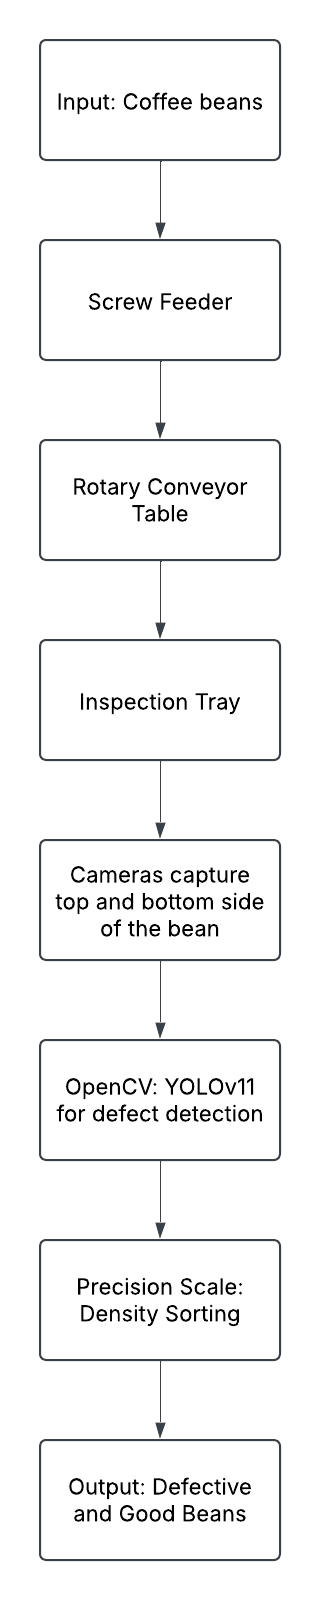
\includegraphics[width=14cm]{ch5/system_block_diagram.png}
    \caption{System Block Diagram}
    \label{fig:system_block_diagram}
\end{figure}

The system is an automated green coffee bean sorting machine, utilizing machine vision. Firstly, the coffee beans are introduced into the system through a funnel, which directs them to a conveyor belt mechanism. The green coffee beans are sorted depending on their visual characteristics. In this process, the physical qualities of the bean are analyzed such as size, color, and defect. If the bean is defective, the system will automatically sort it out. Then, all the non-defective beans will go through the second stage of the system. In the second stage, there will be a precision scale. With the volume and mass of the bean in hand, the density of the bean can be estimated. Depending on the density threshold set by the user, the bean will be classified whether it is good or not.

\begin{figure}[H]
    \centering
    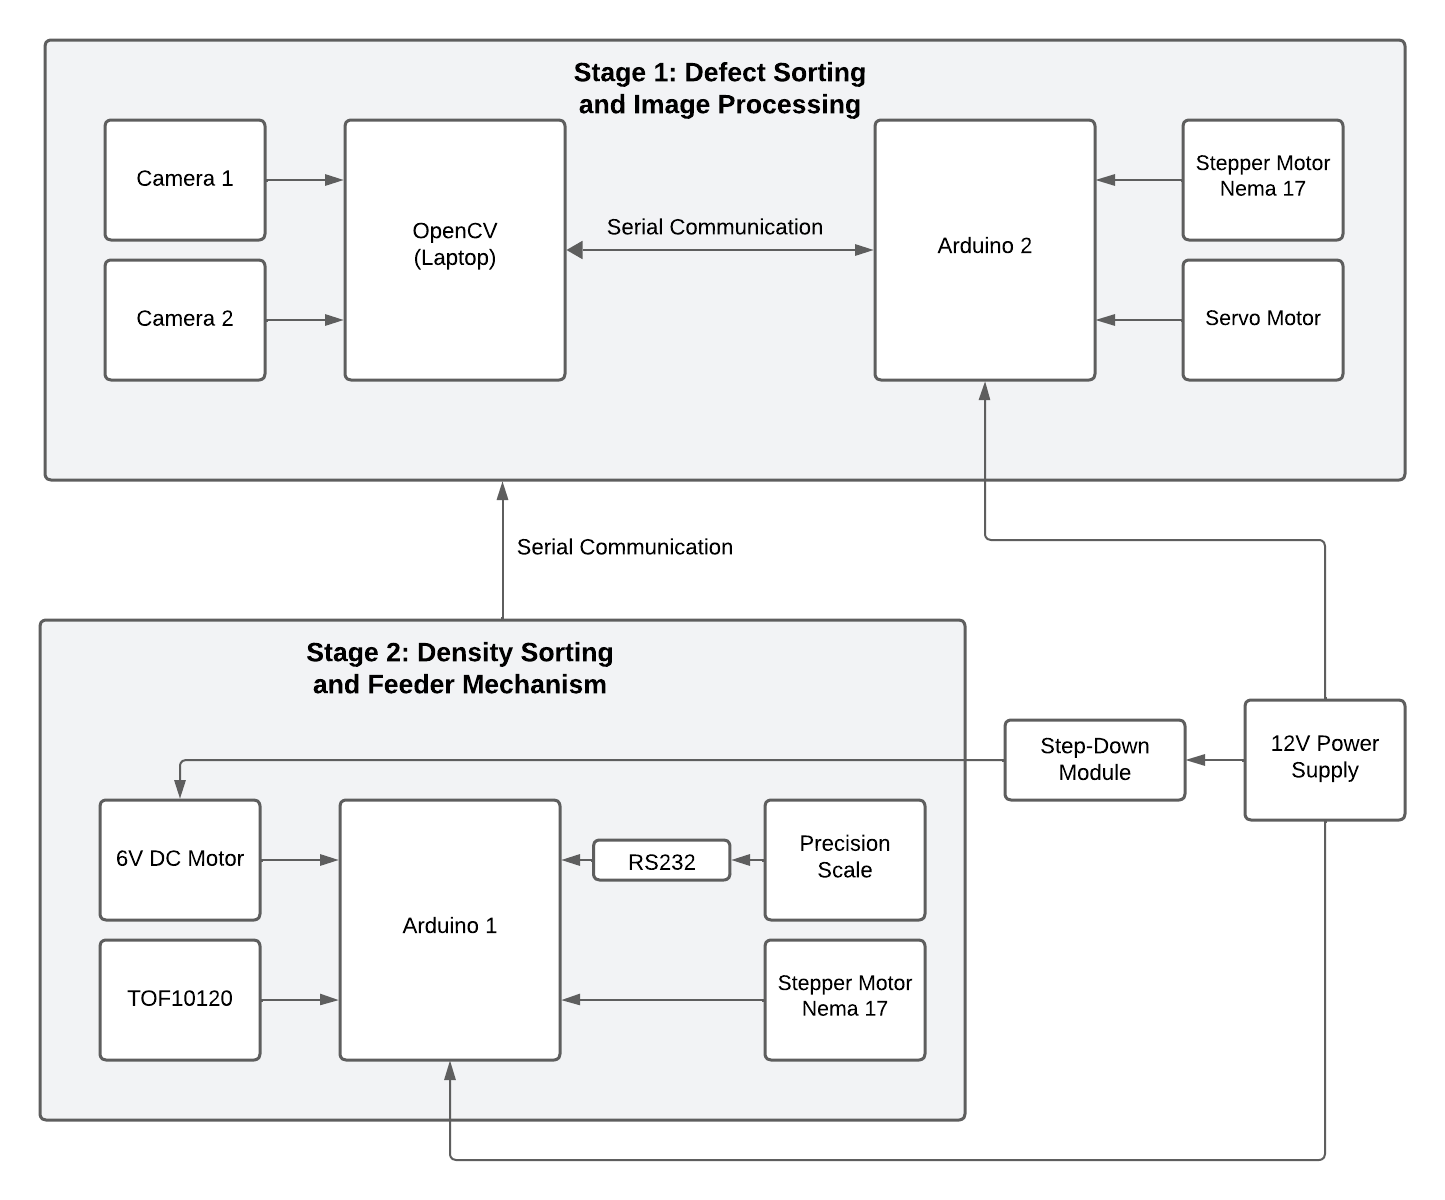
\includegraphics[width=14cm]{ch5/Schematic_Diagram_of_the_System.png}
    \caption{Schematic Diagram of the System}
    \label{fig:system_schematic_diagram}
\end{figure}

Figure \ref{fig:system_schematic_diagram} shows the schematic diagram of the proposed system. Arduino Uno microcontroller makes all the mechanical components such as the servo motor, stepper motors, and the conveyor belt. The servo motor controls the  rotating mechanism for bean sorting. On the other hand, the stepper motors operate a slide mechanism to direct the beans. Two cameras, integrated with OpenCV via Python, handle machine vision algorithms, and image processing for defect detection of the beans. A ToF10120 sensor provides precise distance measurement. A precision weighing scale measures the density of each bean for classification. The Arduino communicates with the OpenCV system through serial communication, ensuring smooth coordination.

\begin{figure}[H]
    \centering
    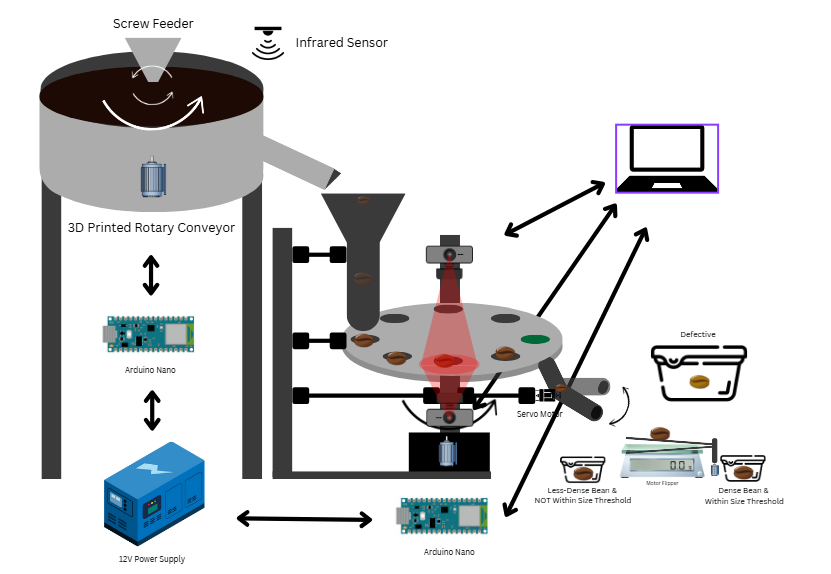
\includegraphics[width=14cm]{ch5/Overview_Of_The_System.png}
    \caption{Design Overview of the System}
    \label{fig:system_design_overview}
\end{figure}

Figure \ref{fig:system_design_overview} shows the design overview of the system. Beans are first arranged through a hopper and a conveyor belt. On top of the conveyor belt, a 3D-printed guide is attached for the beans to maintain a linear formation. Then, the beans are expected to fall into another funnel attached to a tube. The tube is directly attached to a rotating mechanism that allows the beans to be inspected and sorted one-by-one. In this stage, defective beans are sorted out. Then, the non-defective beans are transferred onto the precision scale to analyze the density. The less-dense beans are sorted out of the batch.

\section{Research Design}
\label{sec:research_design}

\begin{figure}[H]
    \centering
    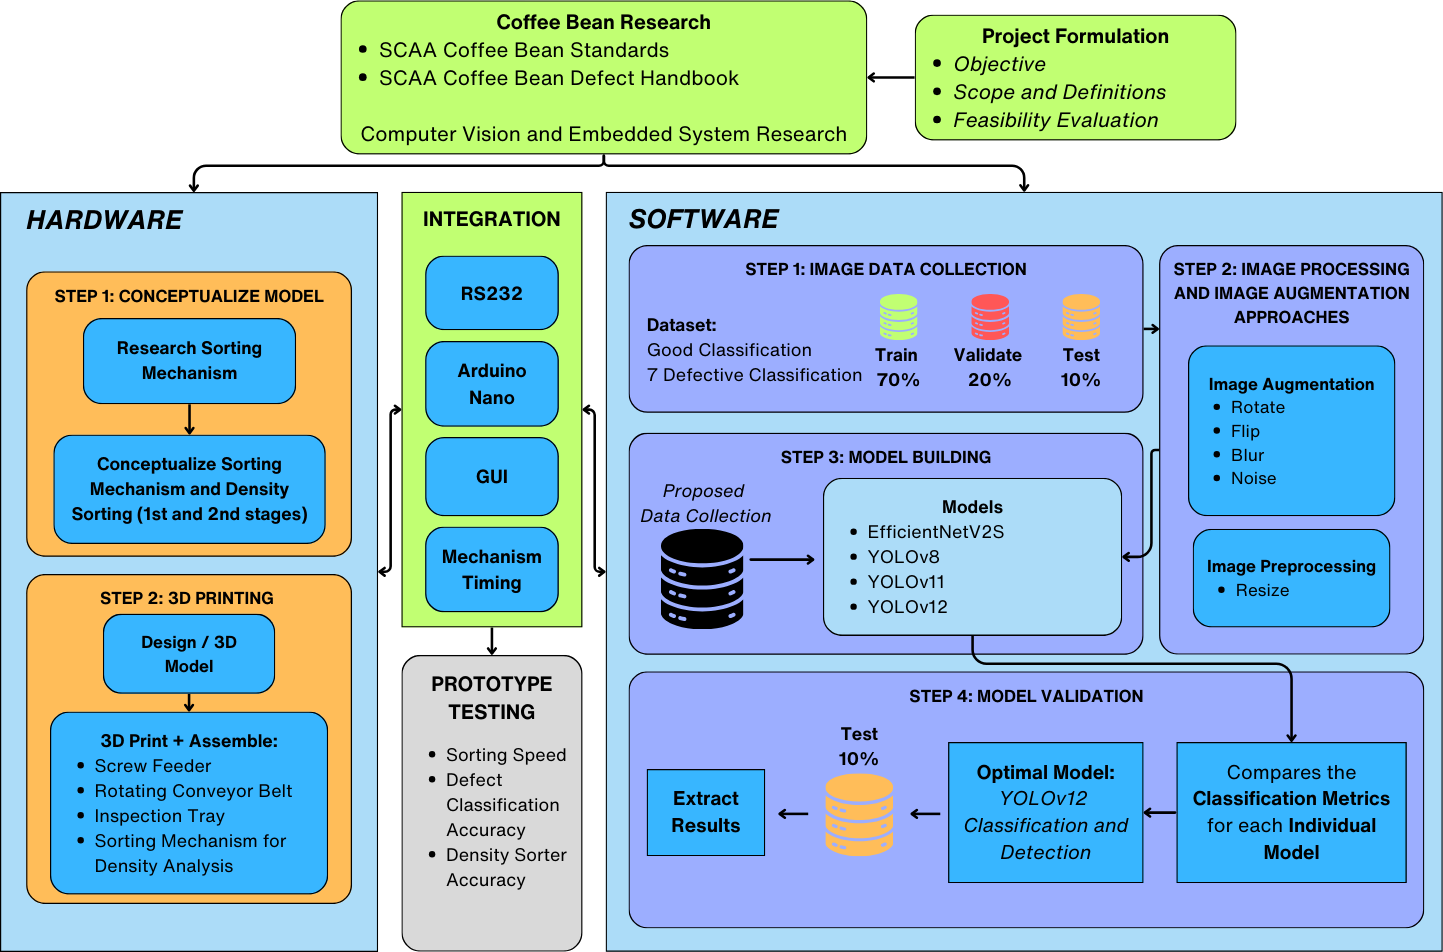
\includegraphics[width=\textwidth]{ch5/DDR_Research_Diagram_v2.png}
    \caption{Design and Development Research (DDR) Methodology}
    \label{fig:ddr_methodology}
\end{figure}

The researchers opted for a Design and Development Research model for the research. As shown in Figure \ref{fig:ddr_methodology},  there are multiple levels that were needed in order to develop a working prototype for the system. 



\section{Dataset Collection}
\label{sec:dataset_collection}

\begin{figure}[H]
    \centering
    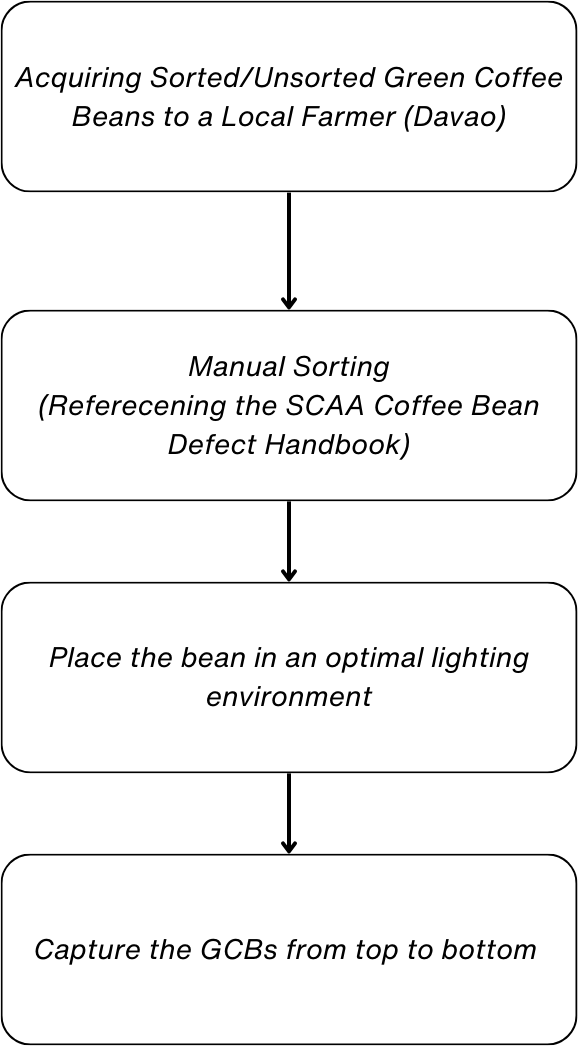
\includegraphics[width=6cm]{ch5/Datacollection_Process.png}
    \caption{Data Collection Process}
    \label{fig:data_collection_process}
\end{figure}
For dataset collection, Arabica green beans from a farm will be used. Each bean will be captured by a high-resolution camera under sufficient and consistent lighting. Proper lighting is crucial, as it directly affects the visibility of the bean’s physical features, minimizing shadows, grain, and other noise that could result from inconsistent illumination. The top and bottom side pictures of the beans are to be collected. In addition, defective beans of the same type and origin will be gathered to identify the different classification of defects (primary and secondary). This study focuses on defects such as Broken, Dried Cherry, Floater, Full Black, Full Sour, Fungus Damage, and Insect Damage. The dataset will include at least 500 images of good beans and a minimum of 200 images for each defect category. To expand the dataset and enhance model training, augmentation techniques such as scaling, rotation, and mirroring will be applied. 

\subsection{Dataset Collection and Model Training}

\begin{figure}[H]
    \centering
    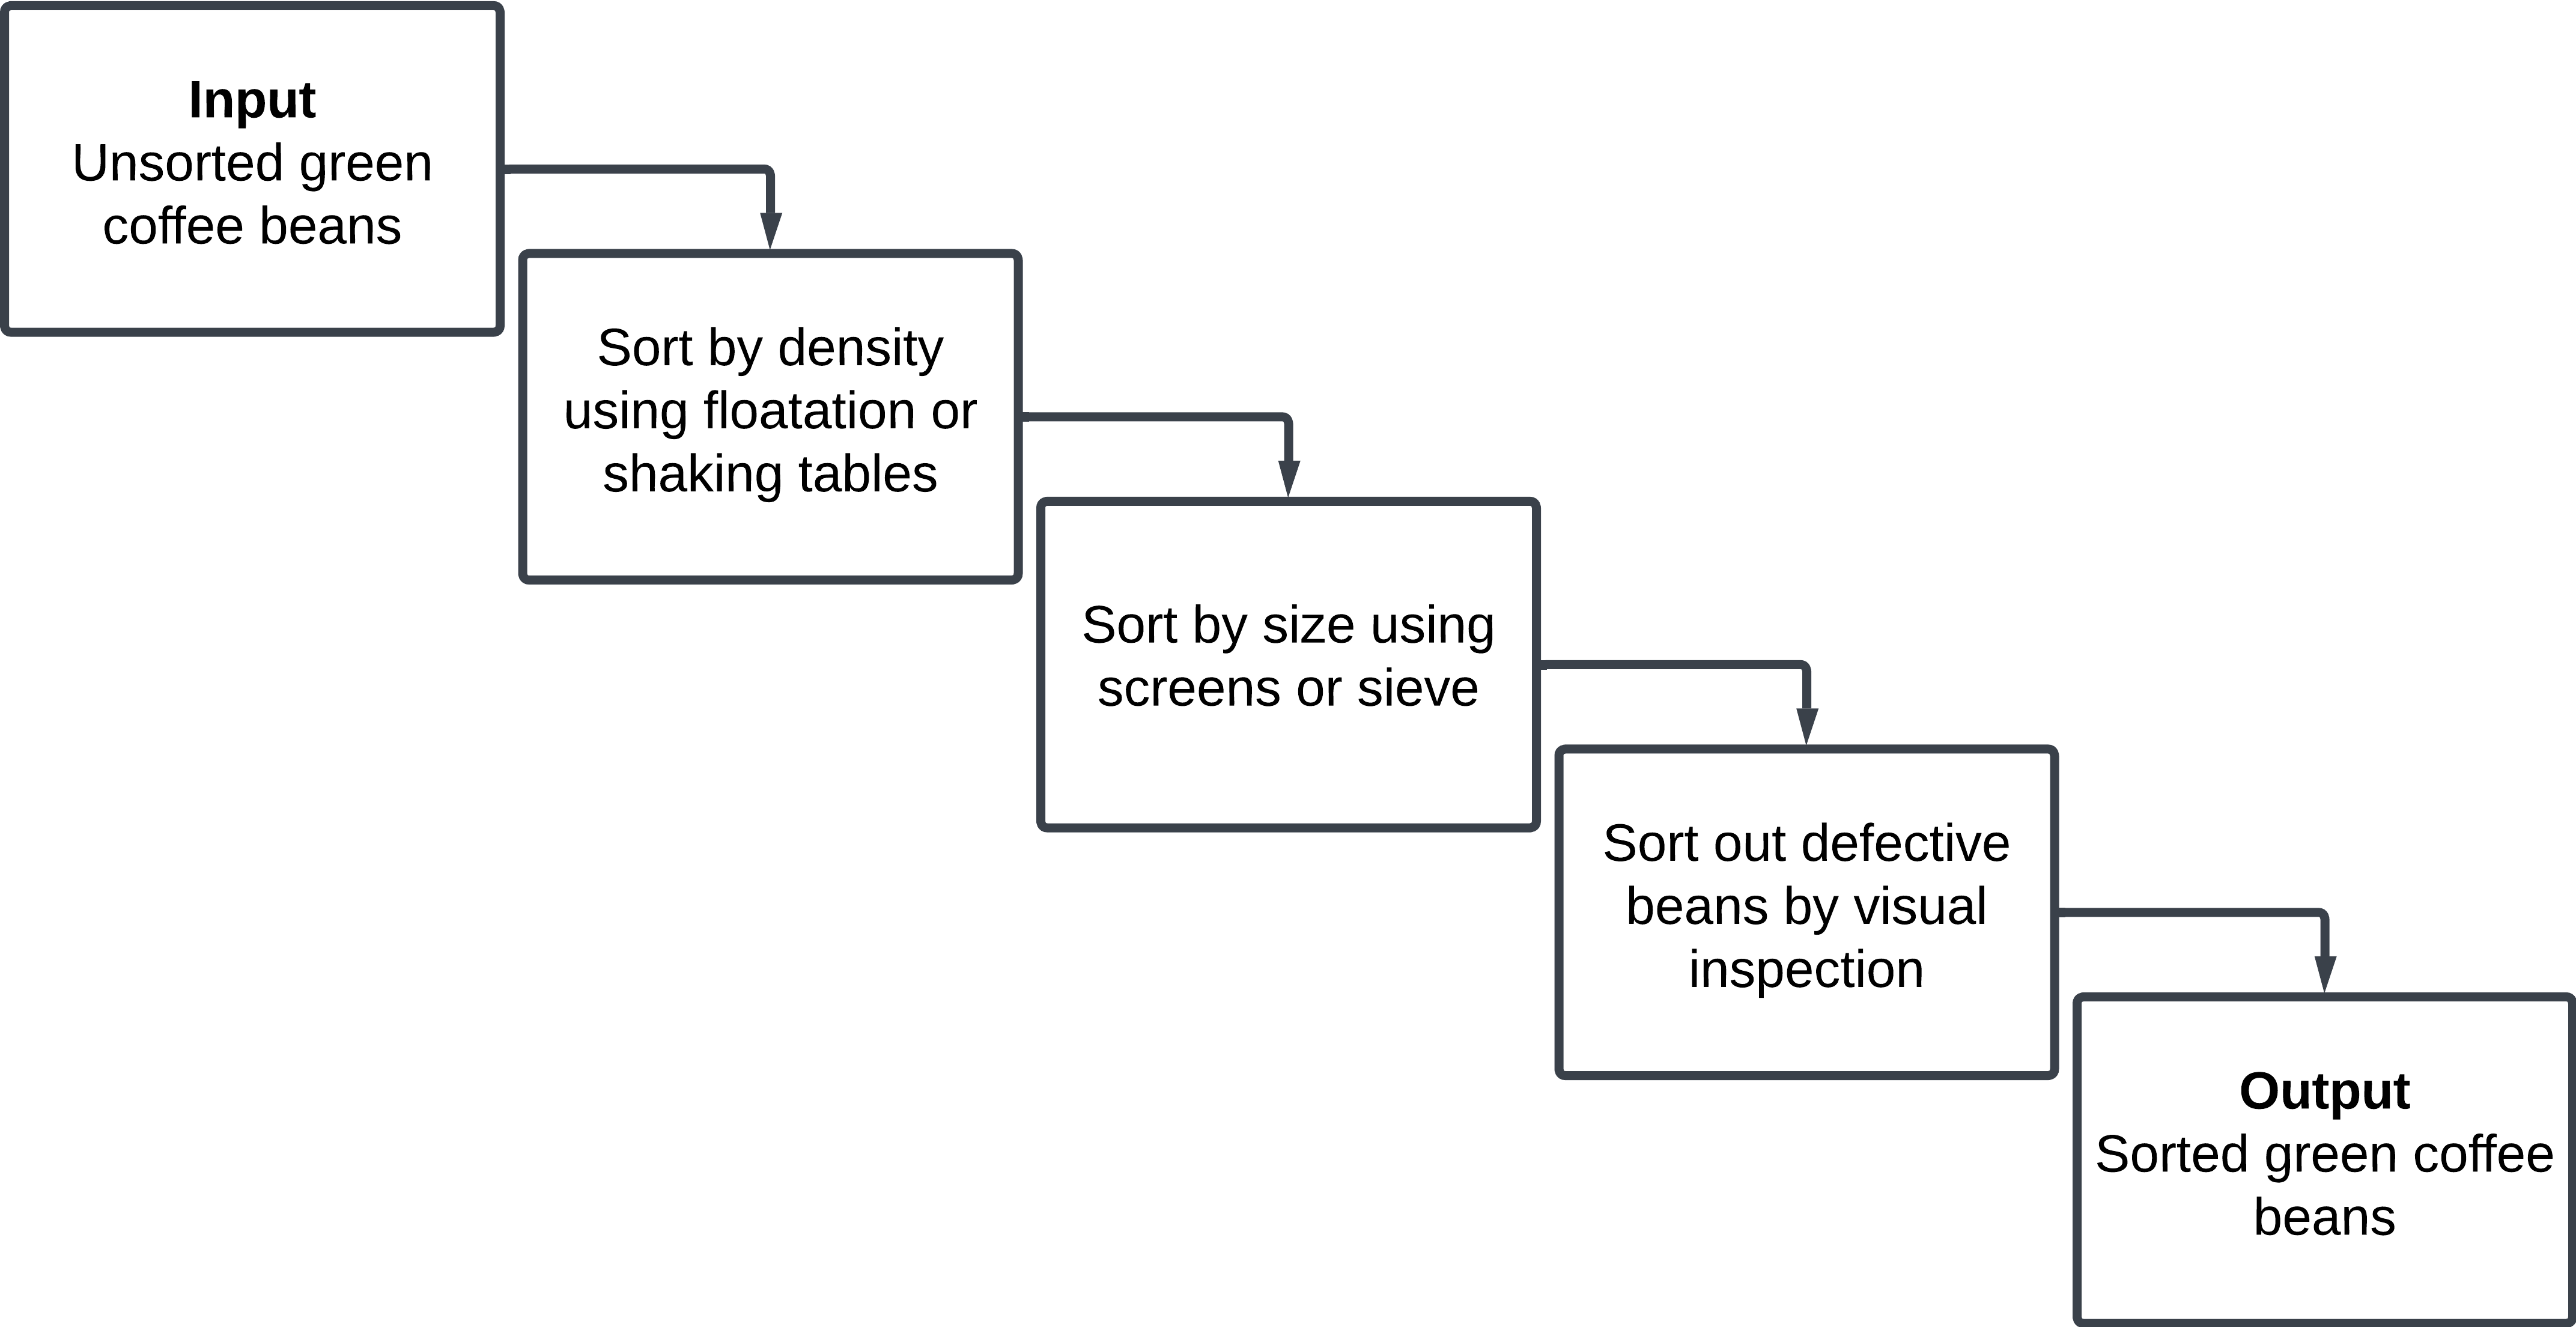
\includegraphics[width=12cm]{ch5/Manual_Sorting_Process.png}
    \caption{Manual Sorting Process}
    \label{fig:manual_sorting}
\end{figure}

% TODO: Fix citations for SCAA
The diagram in Figure \ref{fig:manual_sorting} depicts the representation of the process of manual sorting of unsorted green coffee beans through a series of steps. First, the beans are sorted by density using methods such as floatation or shaking tables. This helps in separating the denser beans, usually pertaining to a more developed and higher quality bean. Then, the beans are sorted by size using screens and sieves with specific dimensions depending on the variety of the beans. After this, a thorough visual inspection is performed by the sorters to identify and remove the defective beans from the batch. To ensure consistency and accuracy, the group follows the Specialty Coffee Association of America (SCAA) Standards Defect Handbook, which provide documentation and guidelines for identifying and classifying defective beans. Finally, the process results in the output of sorted green coffee beans, ready for further processing or sale. 
To ensure the dataset reflects real-world conditions, the group acquired Arabica green coffee beans from Davao. These beans were manually sorted to properly classify defective characteristics before capturing images for dataset creation. This step was crucial for improving the efficiency of batch image capture and ensuring accurate model training, making the system more applicable to Philippine coffee producers.

\subsection{Utilization of Open-Source Database}
% ! CHANGE `the group` statement, citation after Kaggle
To establish a foundation for the system's model, the group initially referenced an open-source dataset from Kaggle. This dataset provides an original 500x500px images of Arabica green coffee beans categorize as defective or good. This dataset also provided insights into how individual beans were captured, including factors such as lighting, camera positioning, focus, and resolution. By analyzing the dataset, the group gained a better understanding of how to achieve a high-quality data collection, ensuring that the collected dataset would contribute to high model accuracy when it is fed into the system.


\subsection{First Iteration of Dataset Collection}
\begin{figure}[H]
    \centering
    \includegraphics[width=10cm]{data_collection_setup.png}
    \caption{First Iteration of Data Collection Setup}
    \label{fig:data_collection_setup}
\end{figure}

\begin{figure}[H]
	\centering
	\begin{tabular}{cc}
		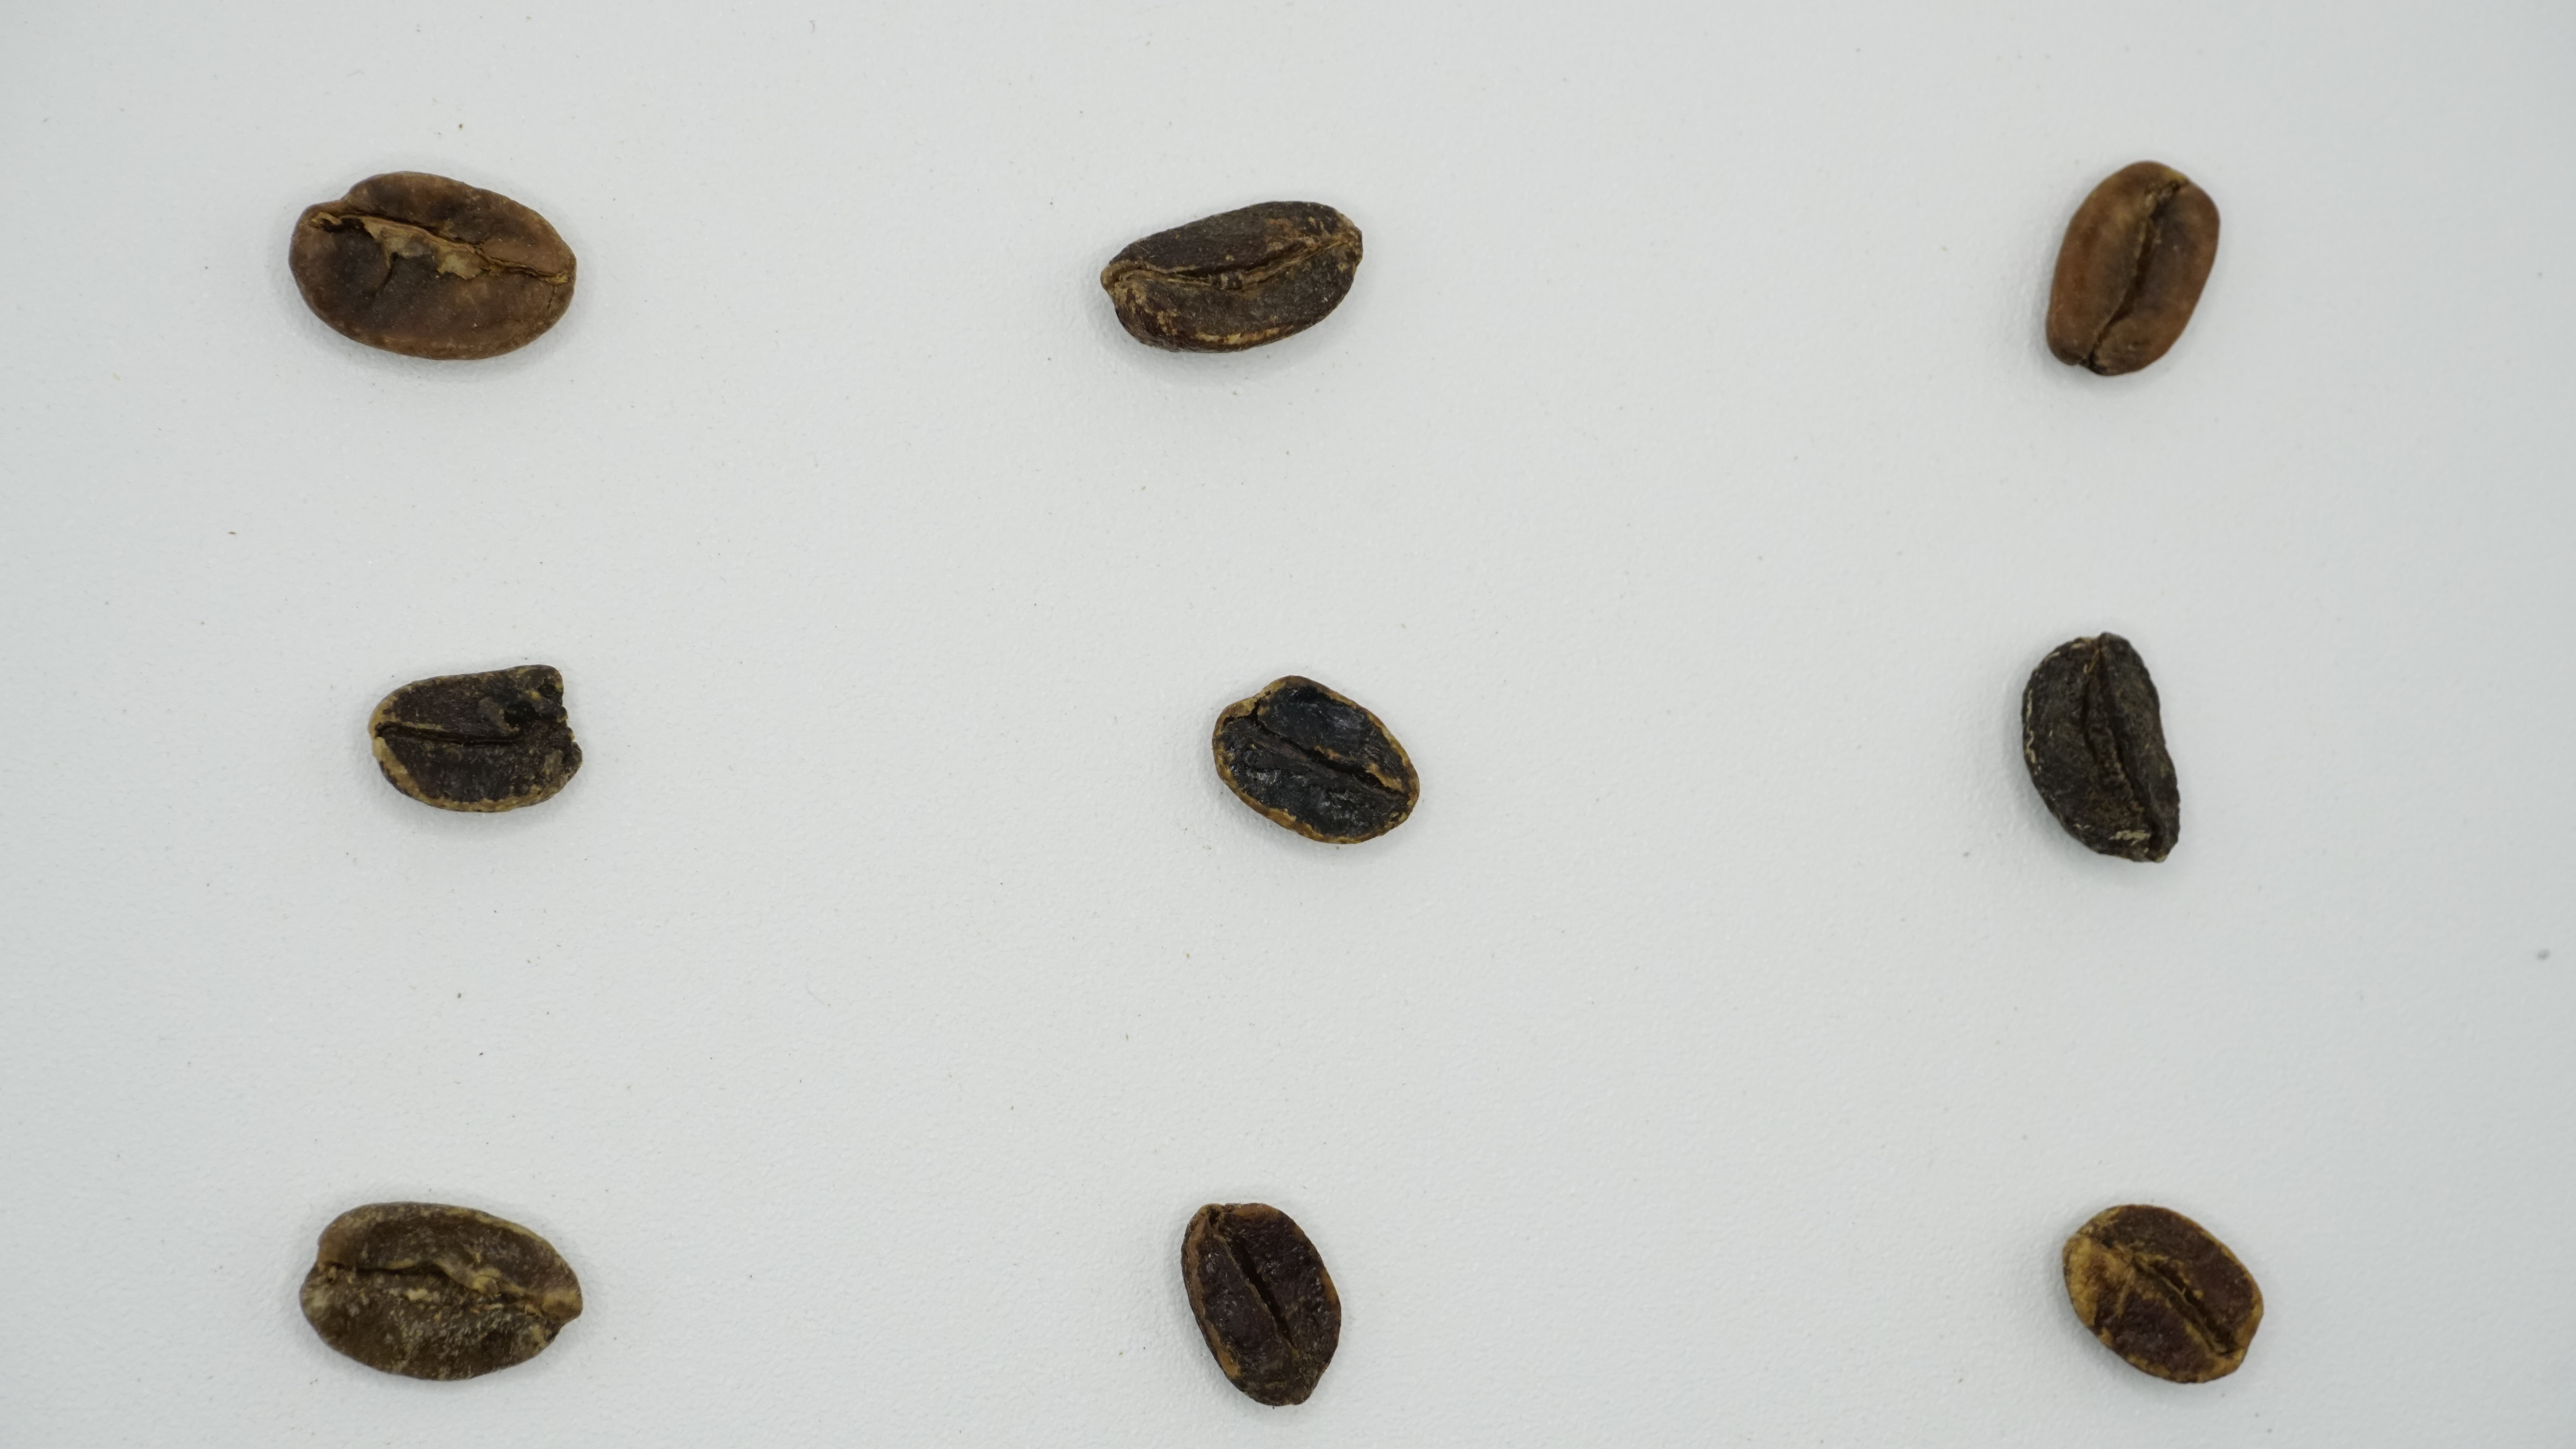
\includegraphics[width=0.3\textwidth]{ch5/1st-Iteration-Table/Black.JPG} &
		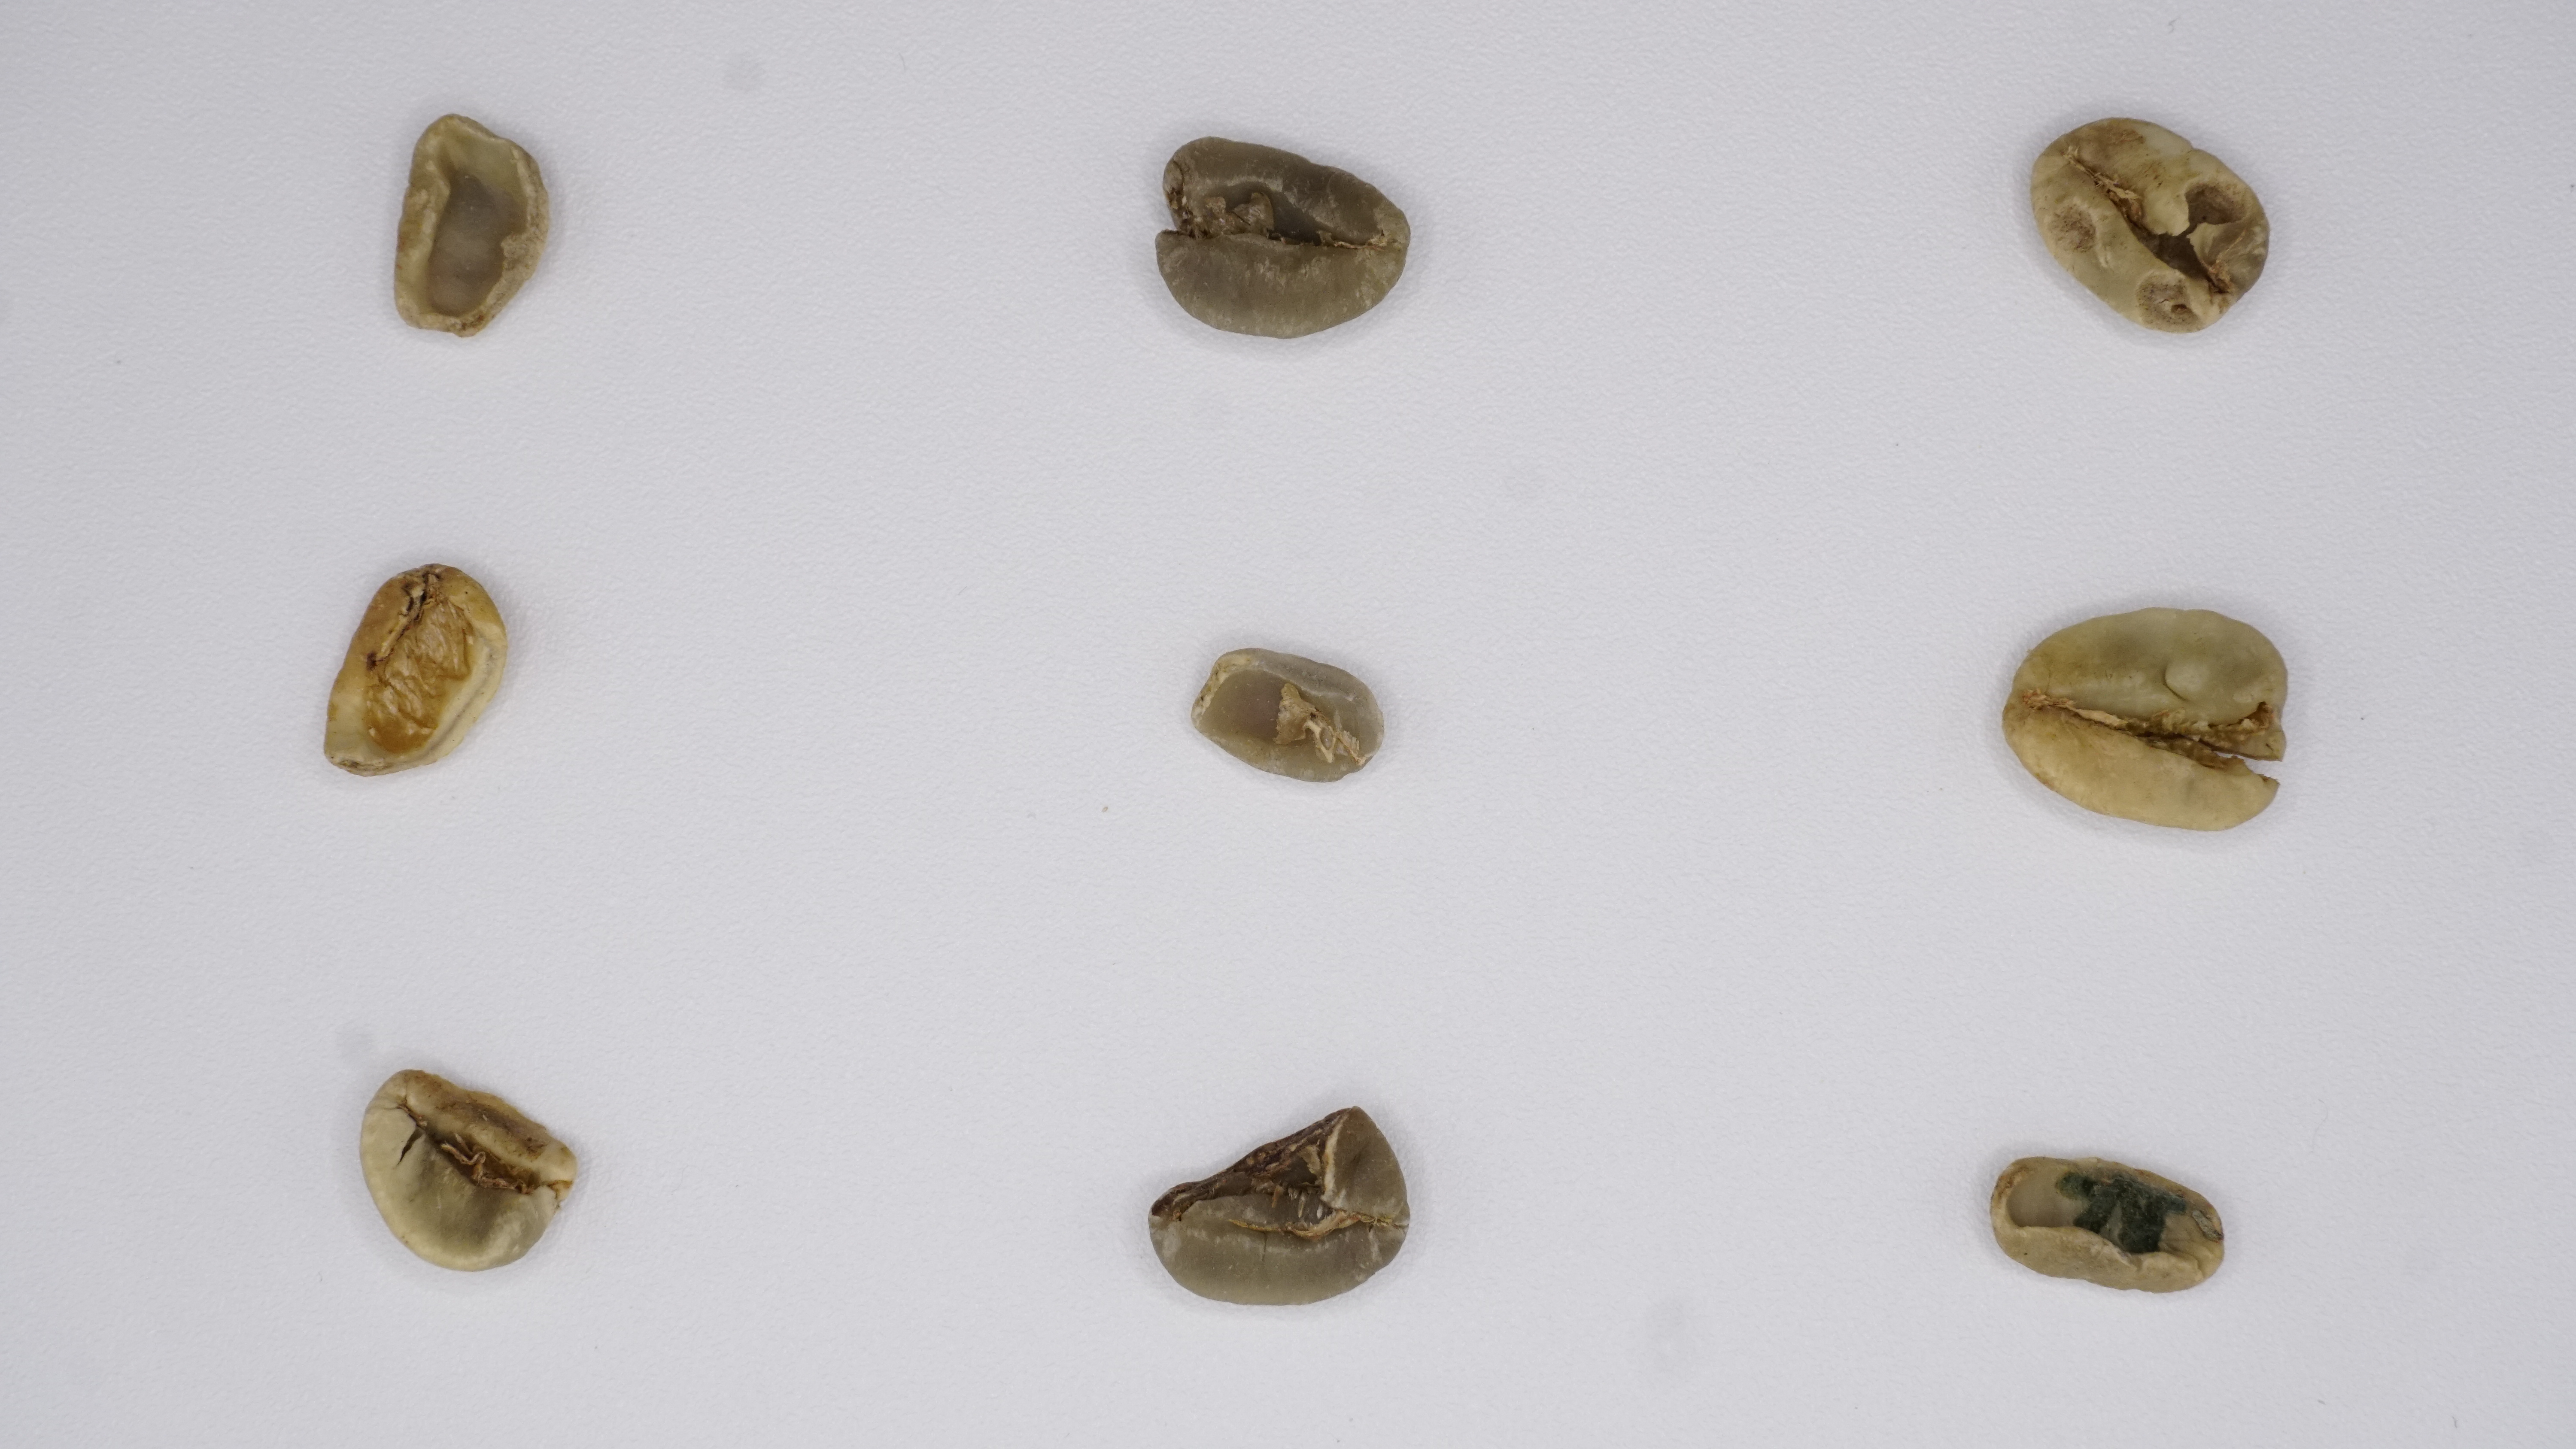
\includegraphics[width=0.3\textwidth]{ch5/1st-Iteration-Table/Broken.JPG} \\
		\textbf{Black}  & \textbf{Broken} \\[6pt]
	\end{tabular}
	\begin{tabular}{cc}
		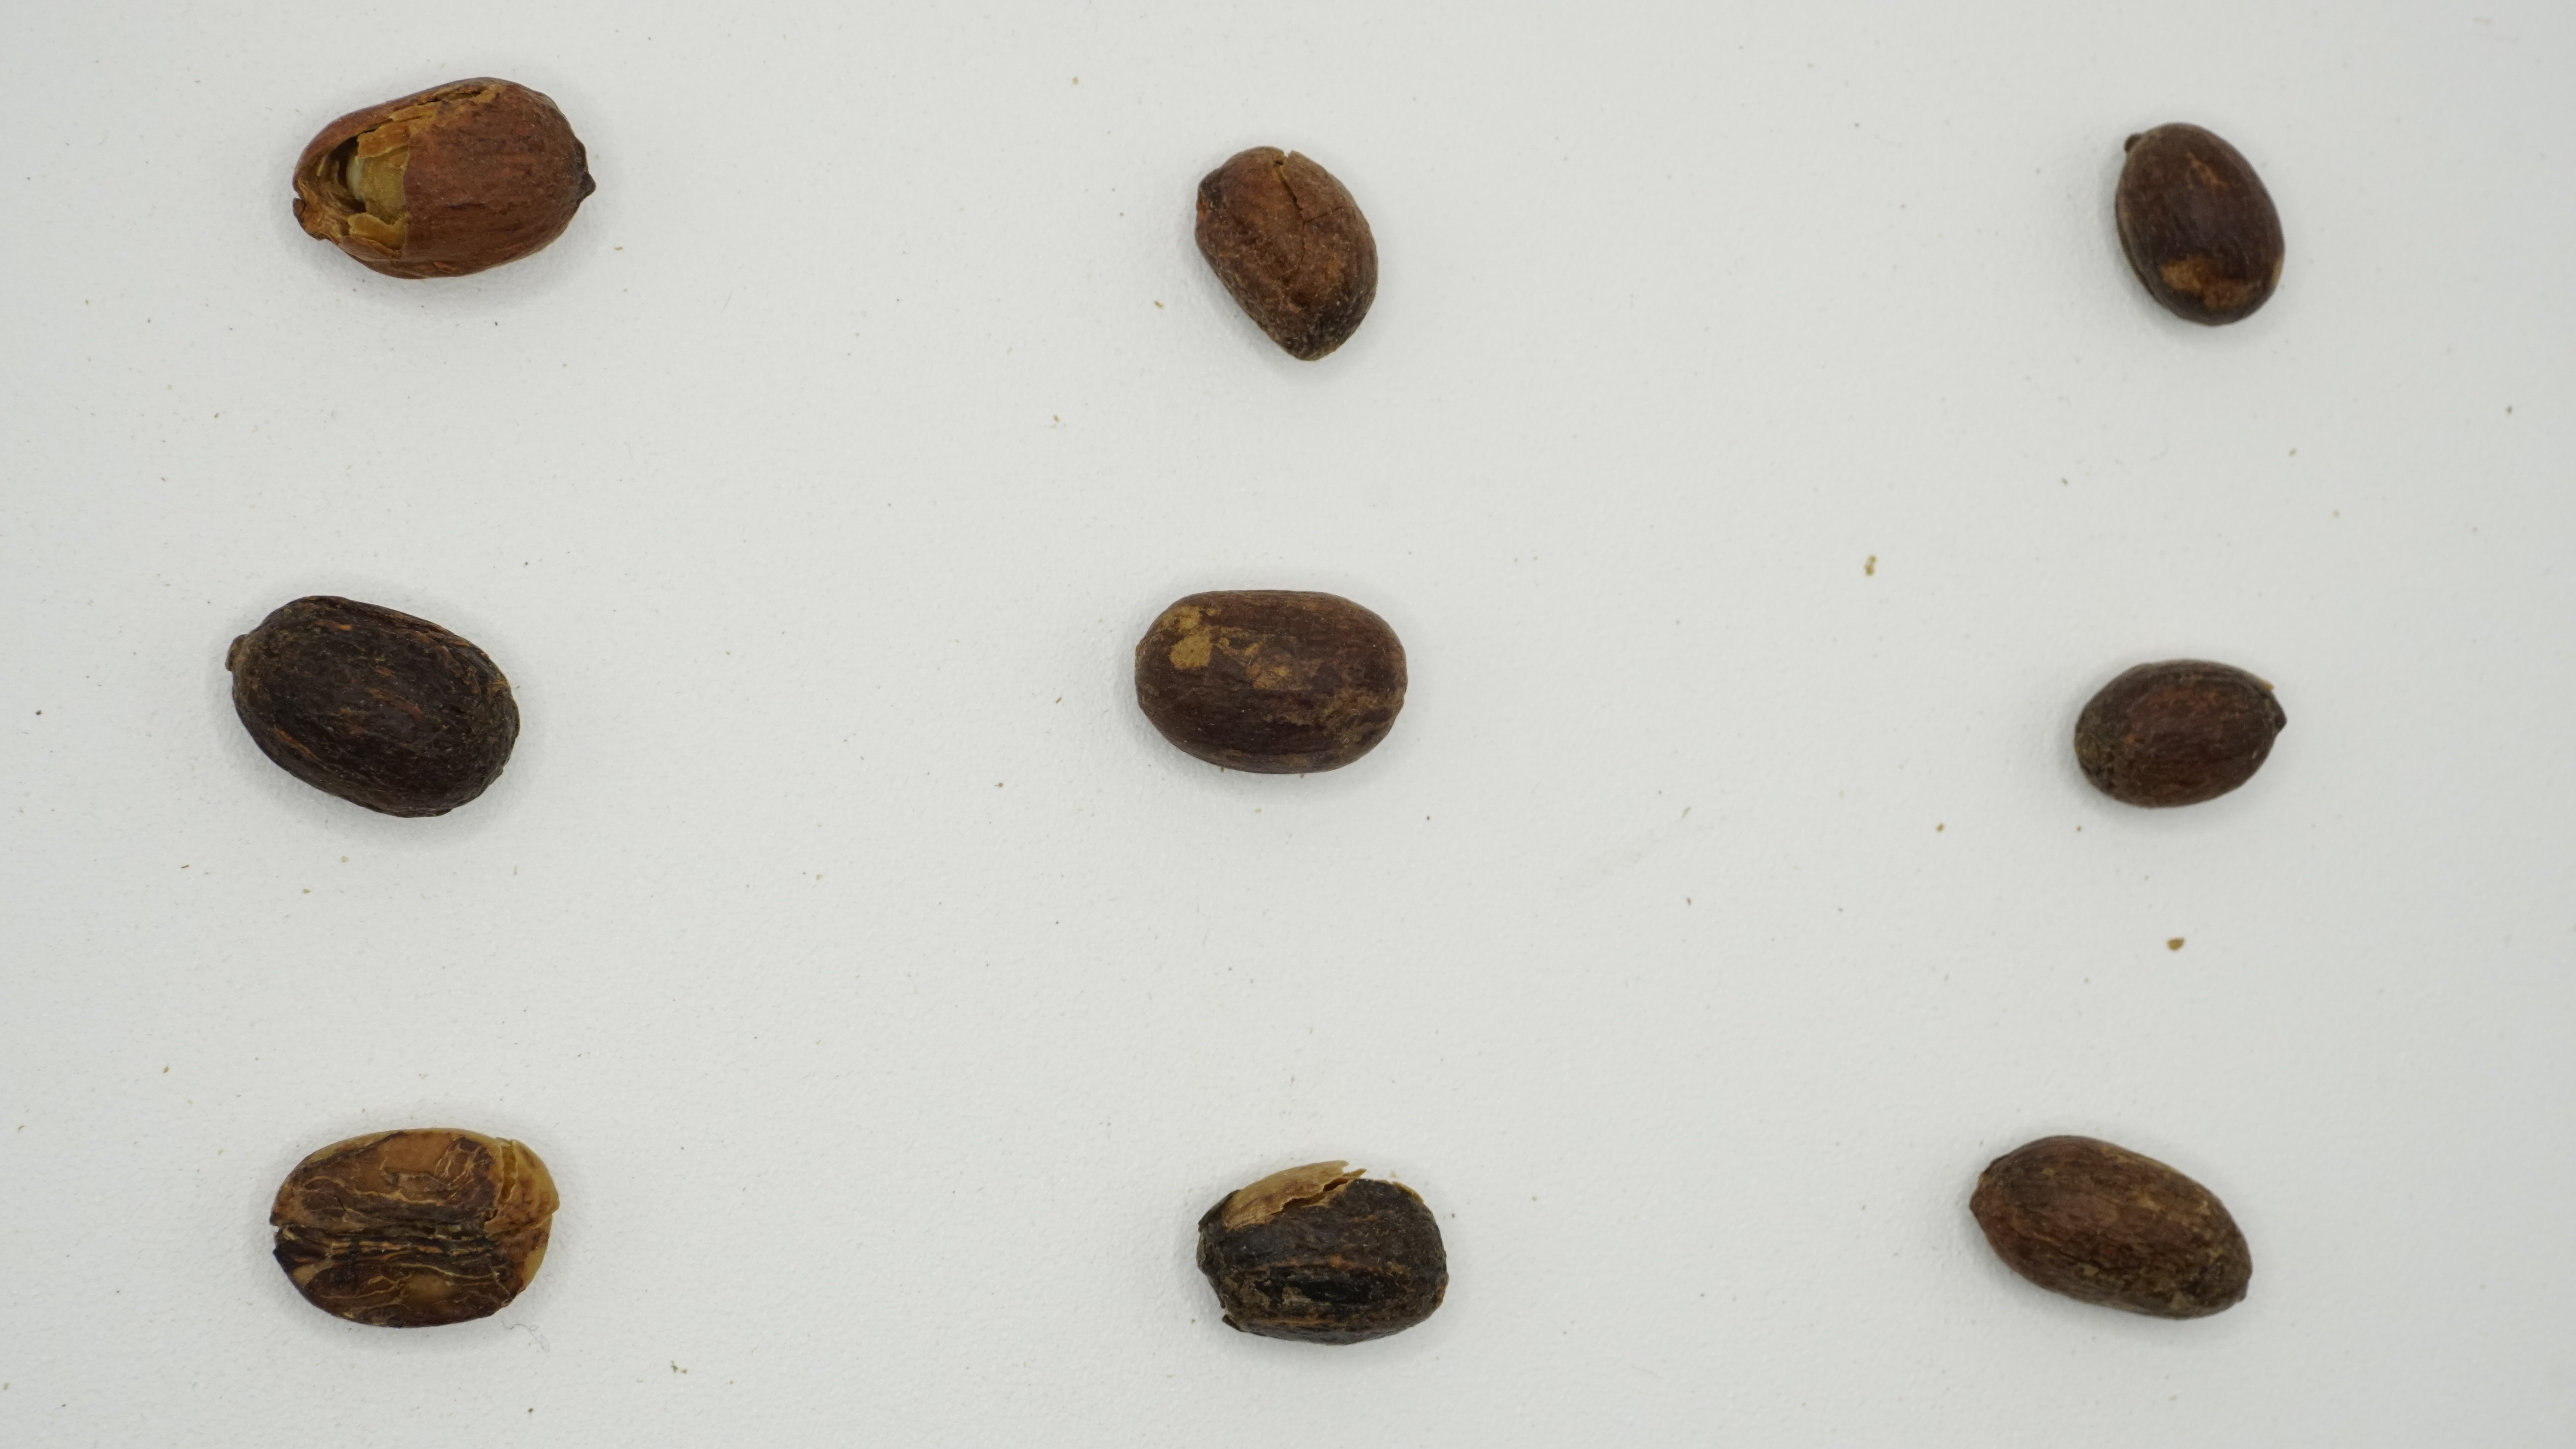
\includegraphics[width=0.3\textwidth]{ch5/1st-Iteration-Table/DriedCherry.JPG} &
		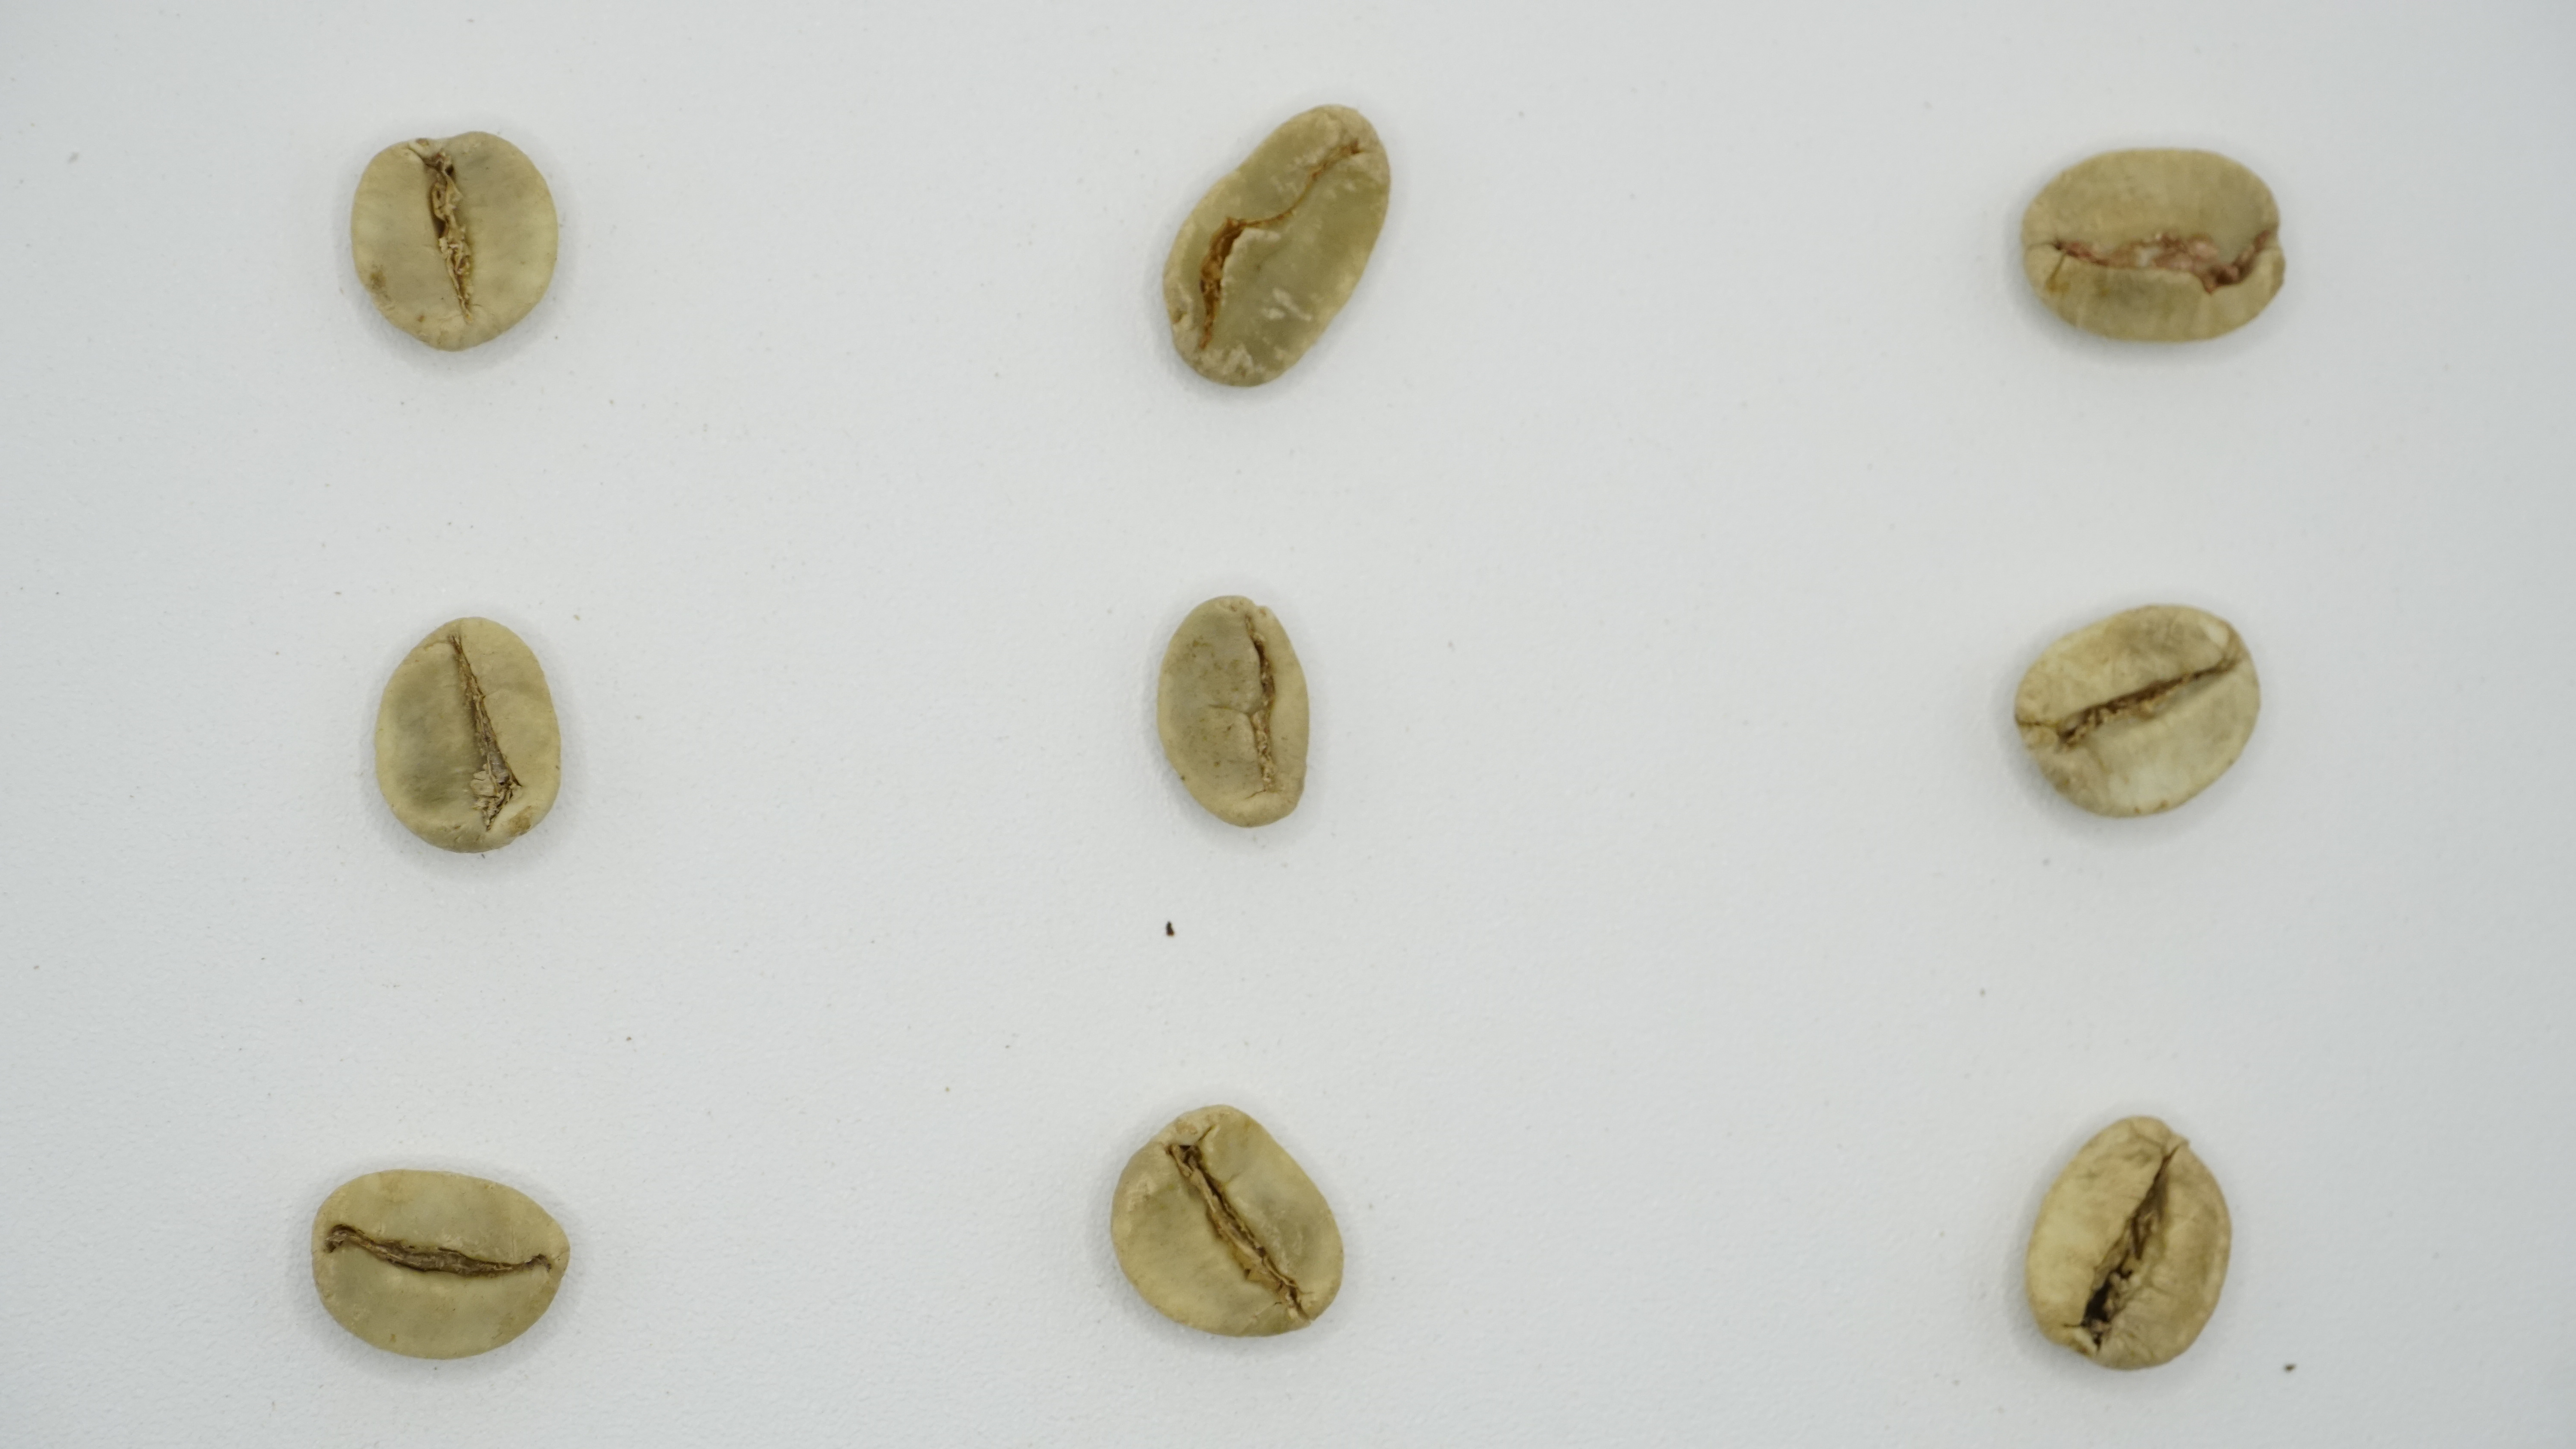
\includegraphics[width=0.3\textwidth]{ch5/1st-Iteration-Table/Floater.JPG} \\
		\textbf{Dried Cherry}  & \textbf{Floater} \\[6pt]
	\end{tabular}
	\begin{tabular}{cc}
		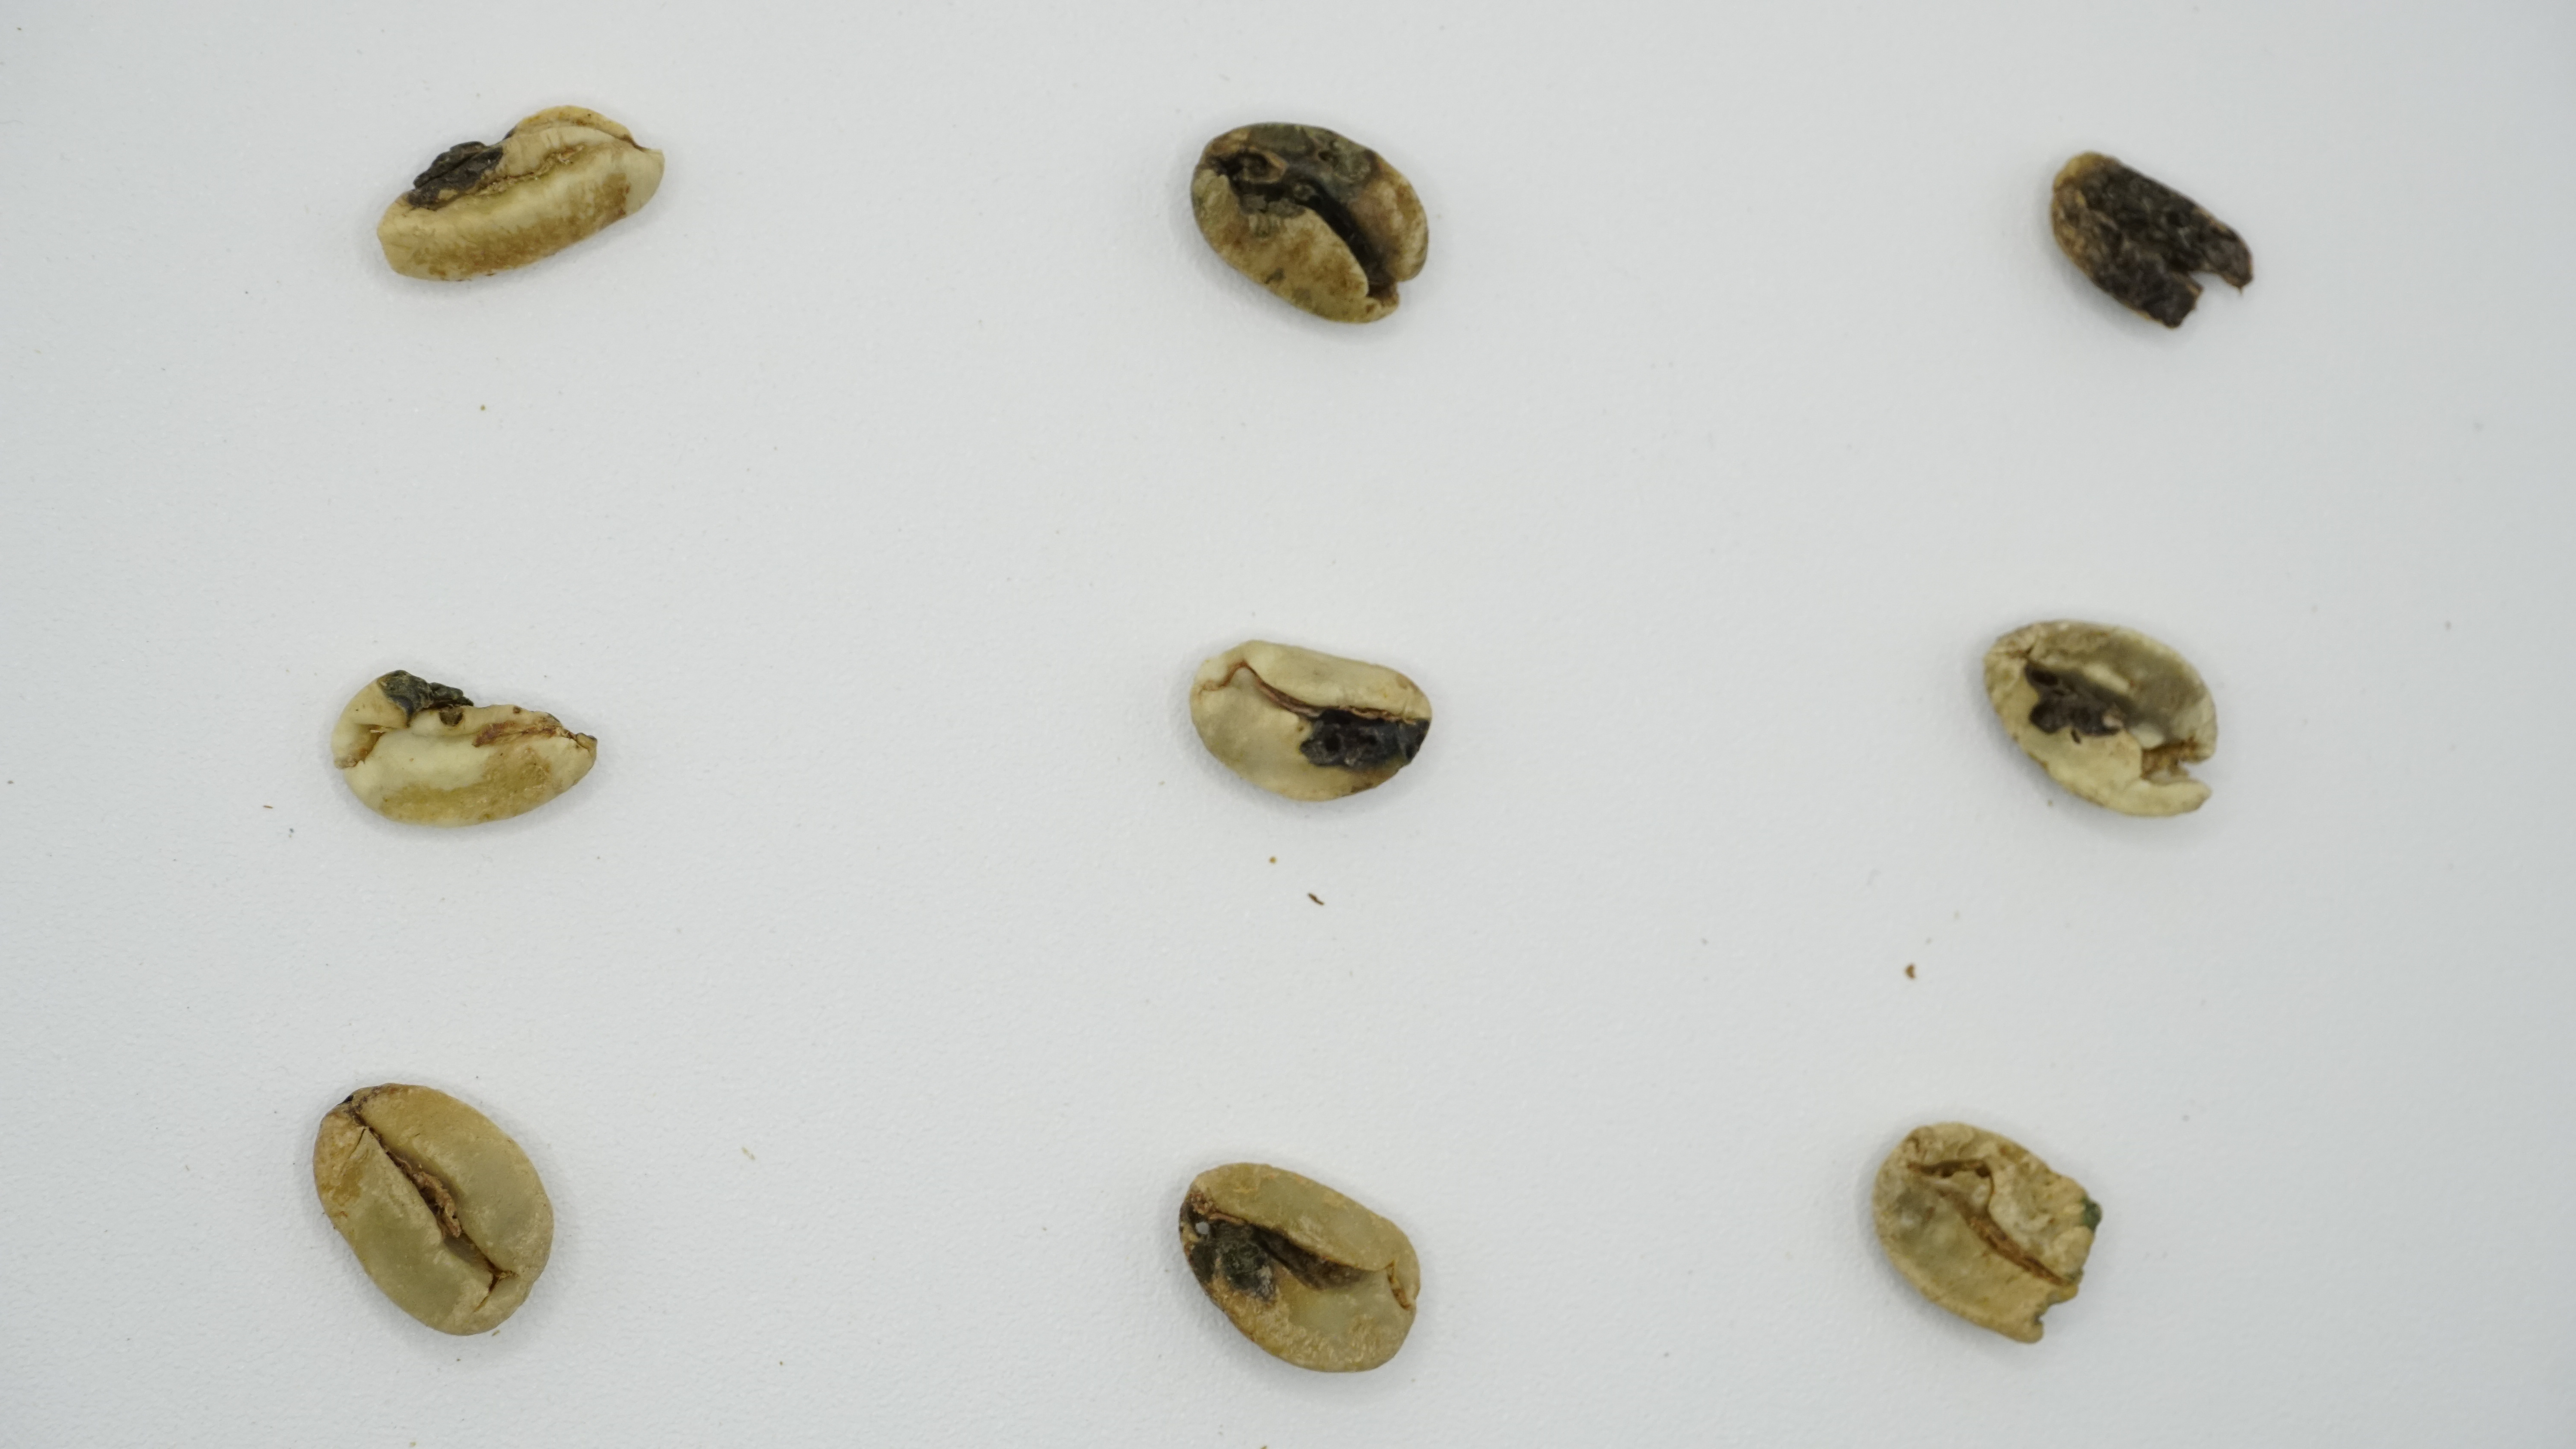
\includegraphics[width=0.3\textwidth]{ch5/1st-Iteration-Table/FungusDamage.JPG} &
		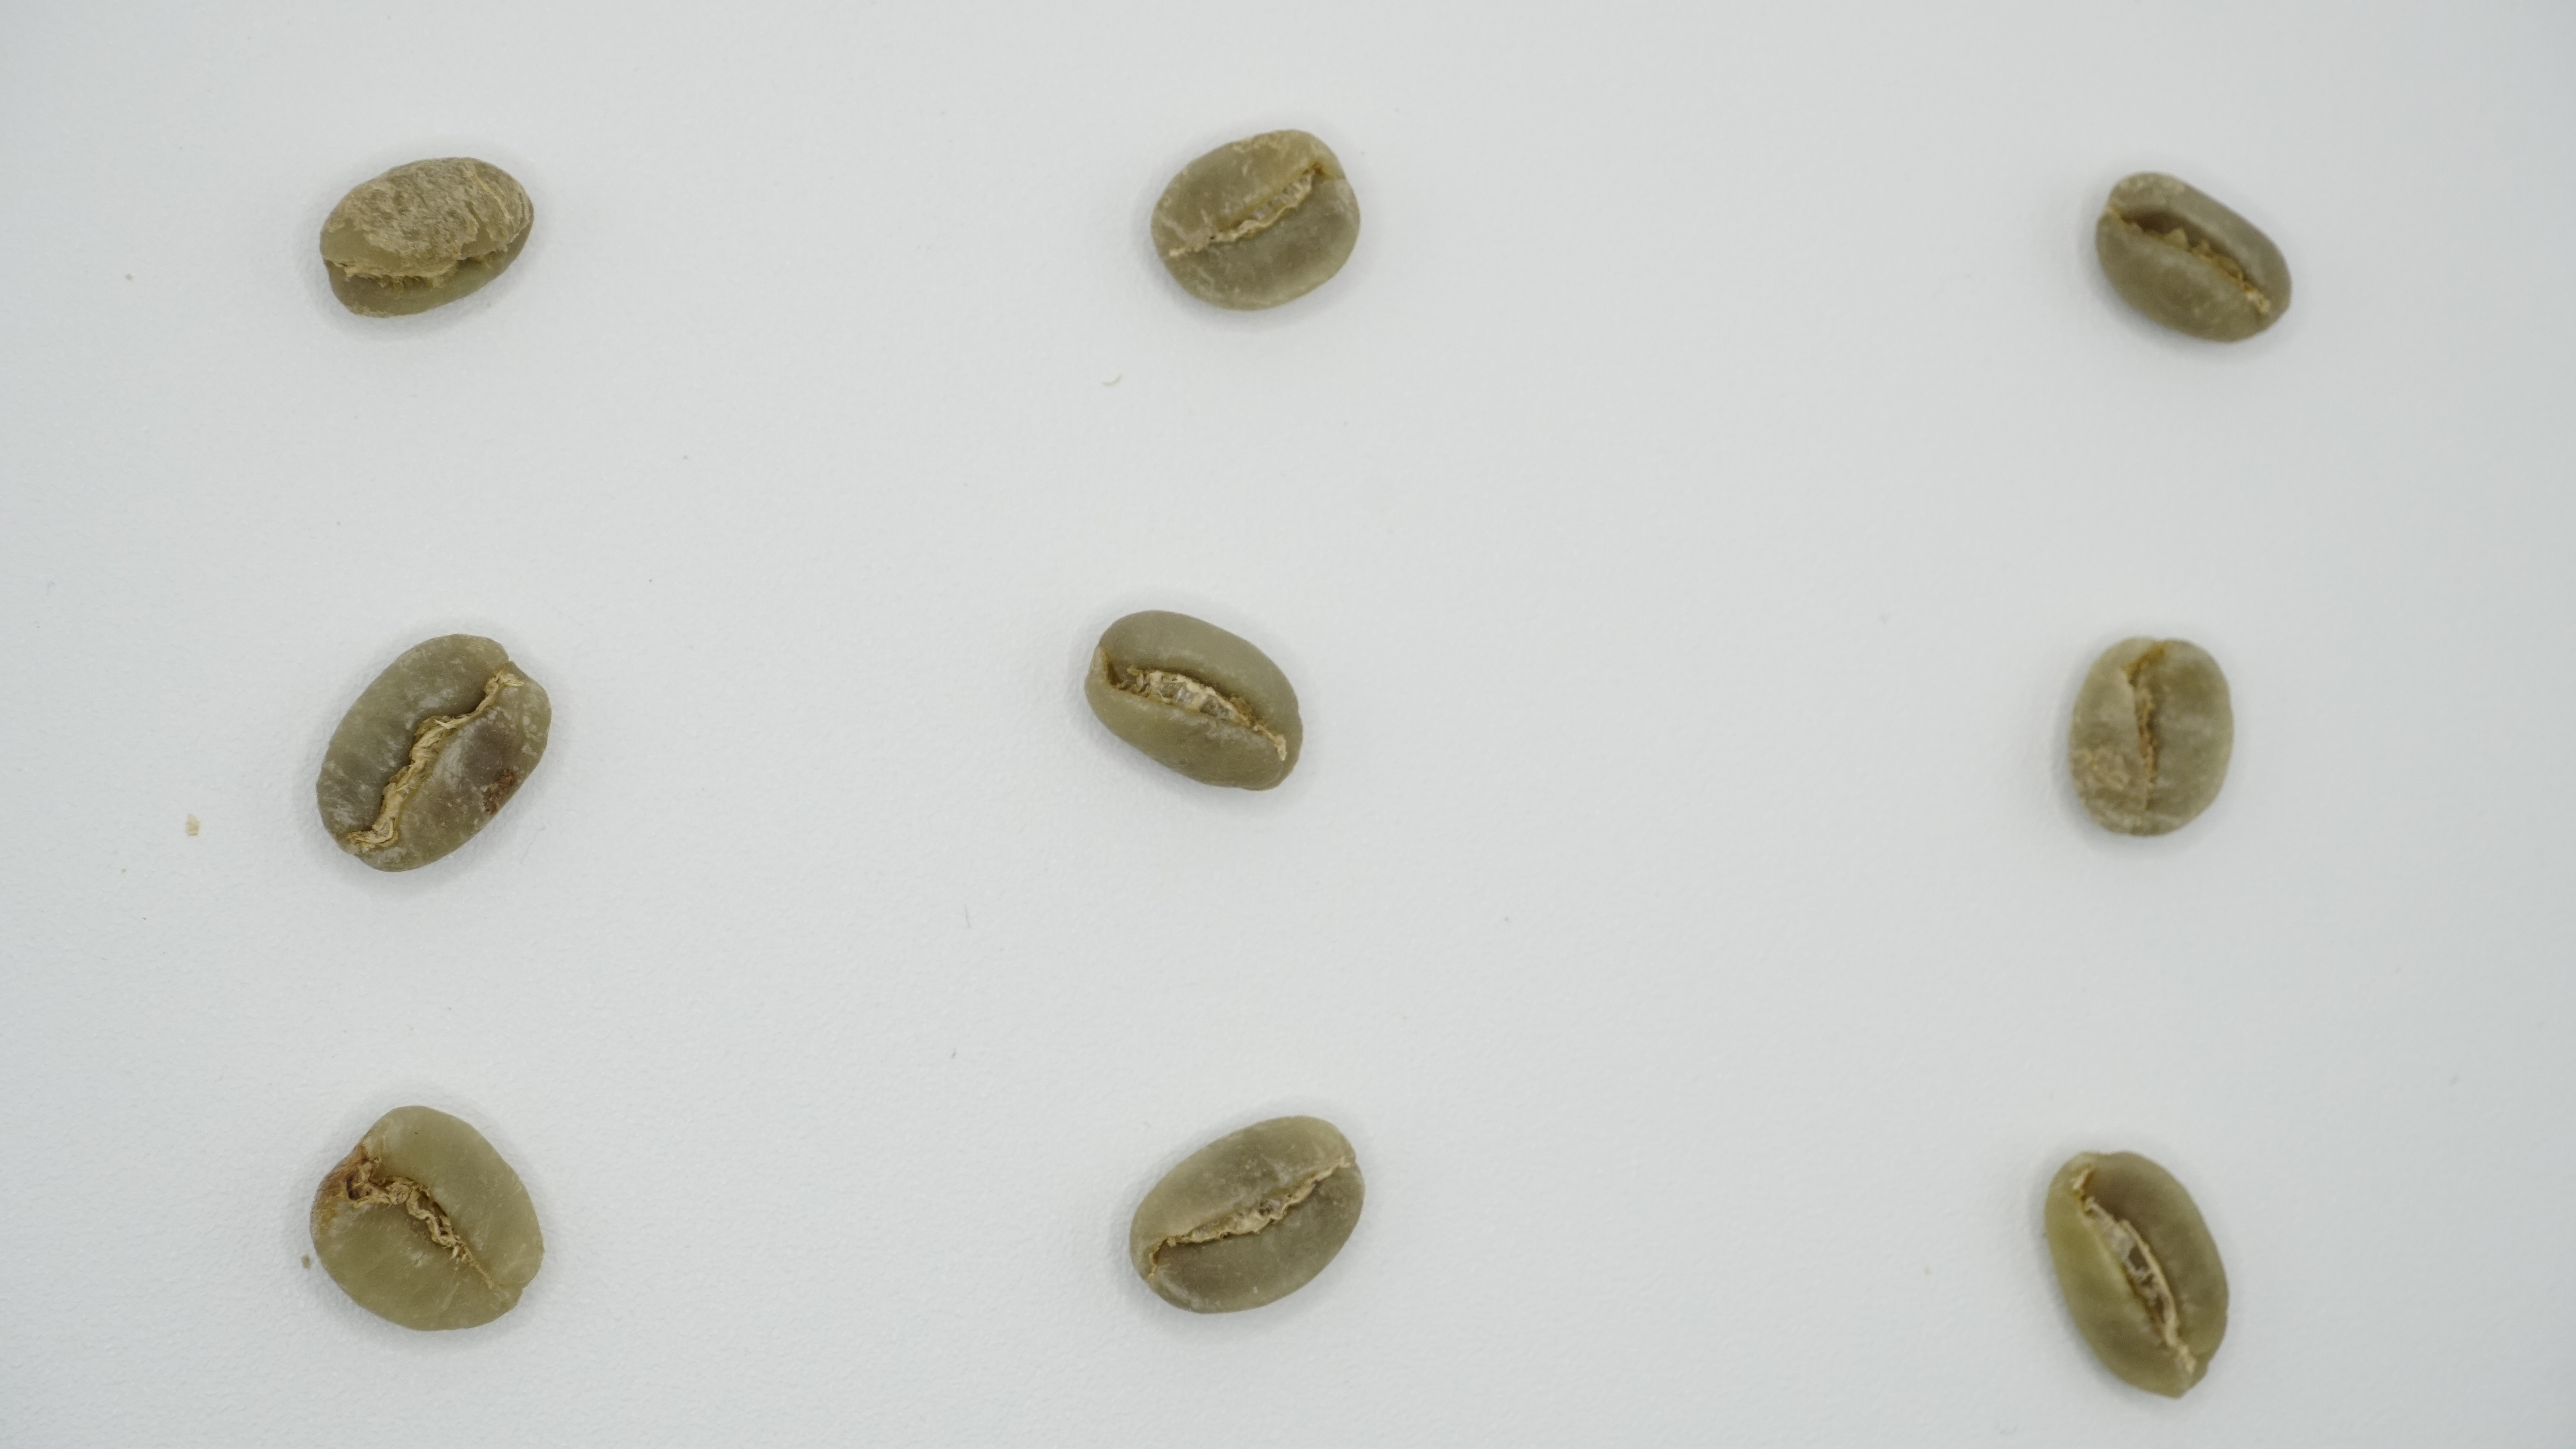
\includegraphics[width=0.3\textwidth]{ch5/1st-Iteration-Table/Good.JPG} \\
		\textbf{Fungus Damage}  & \textbf{Good} \\[6pt]
	\end{tabular}
	\begin{tabular}{cc}
		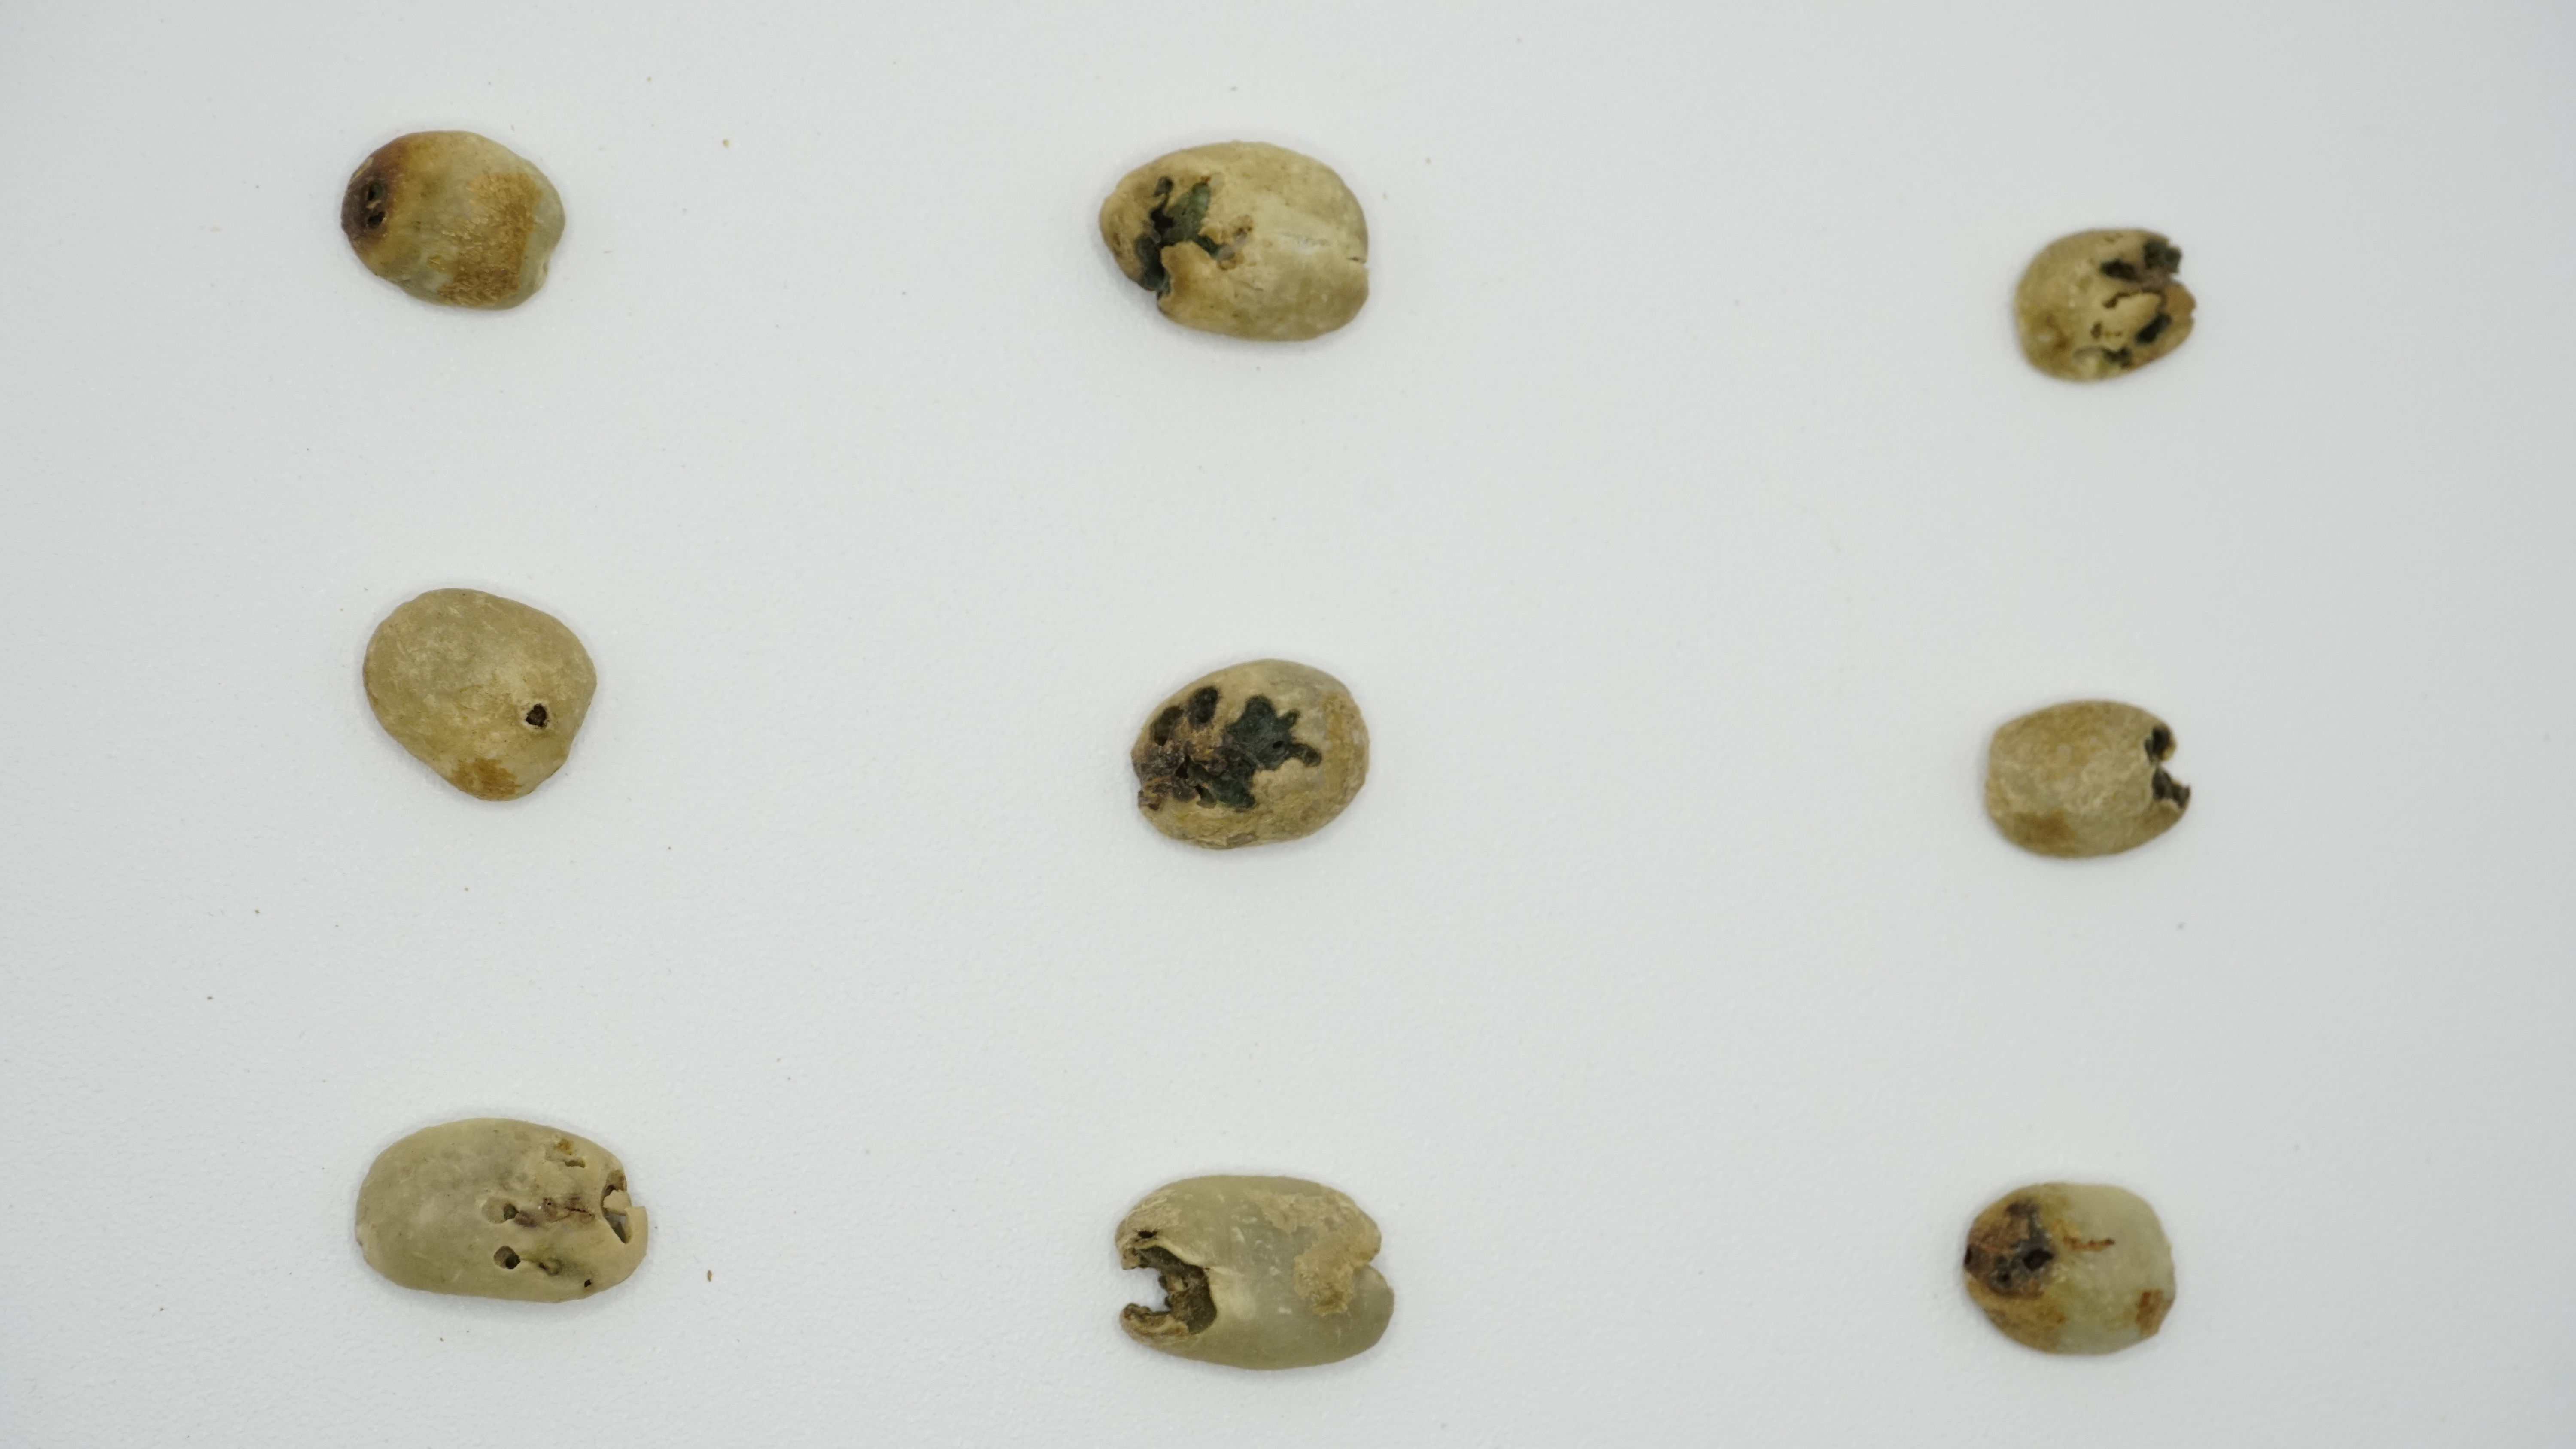
\includegraphics[width=0.3\textwidth]{ch5/1st-Iteration-Table/InsectDamage.JPG} &
		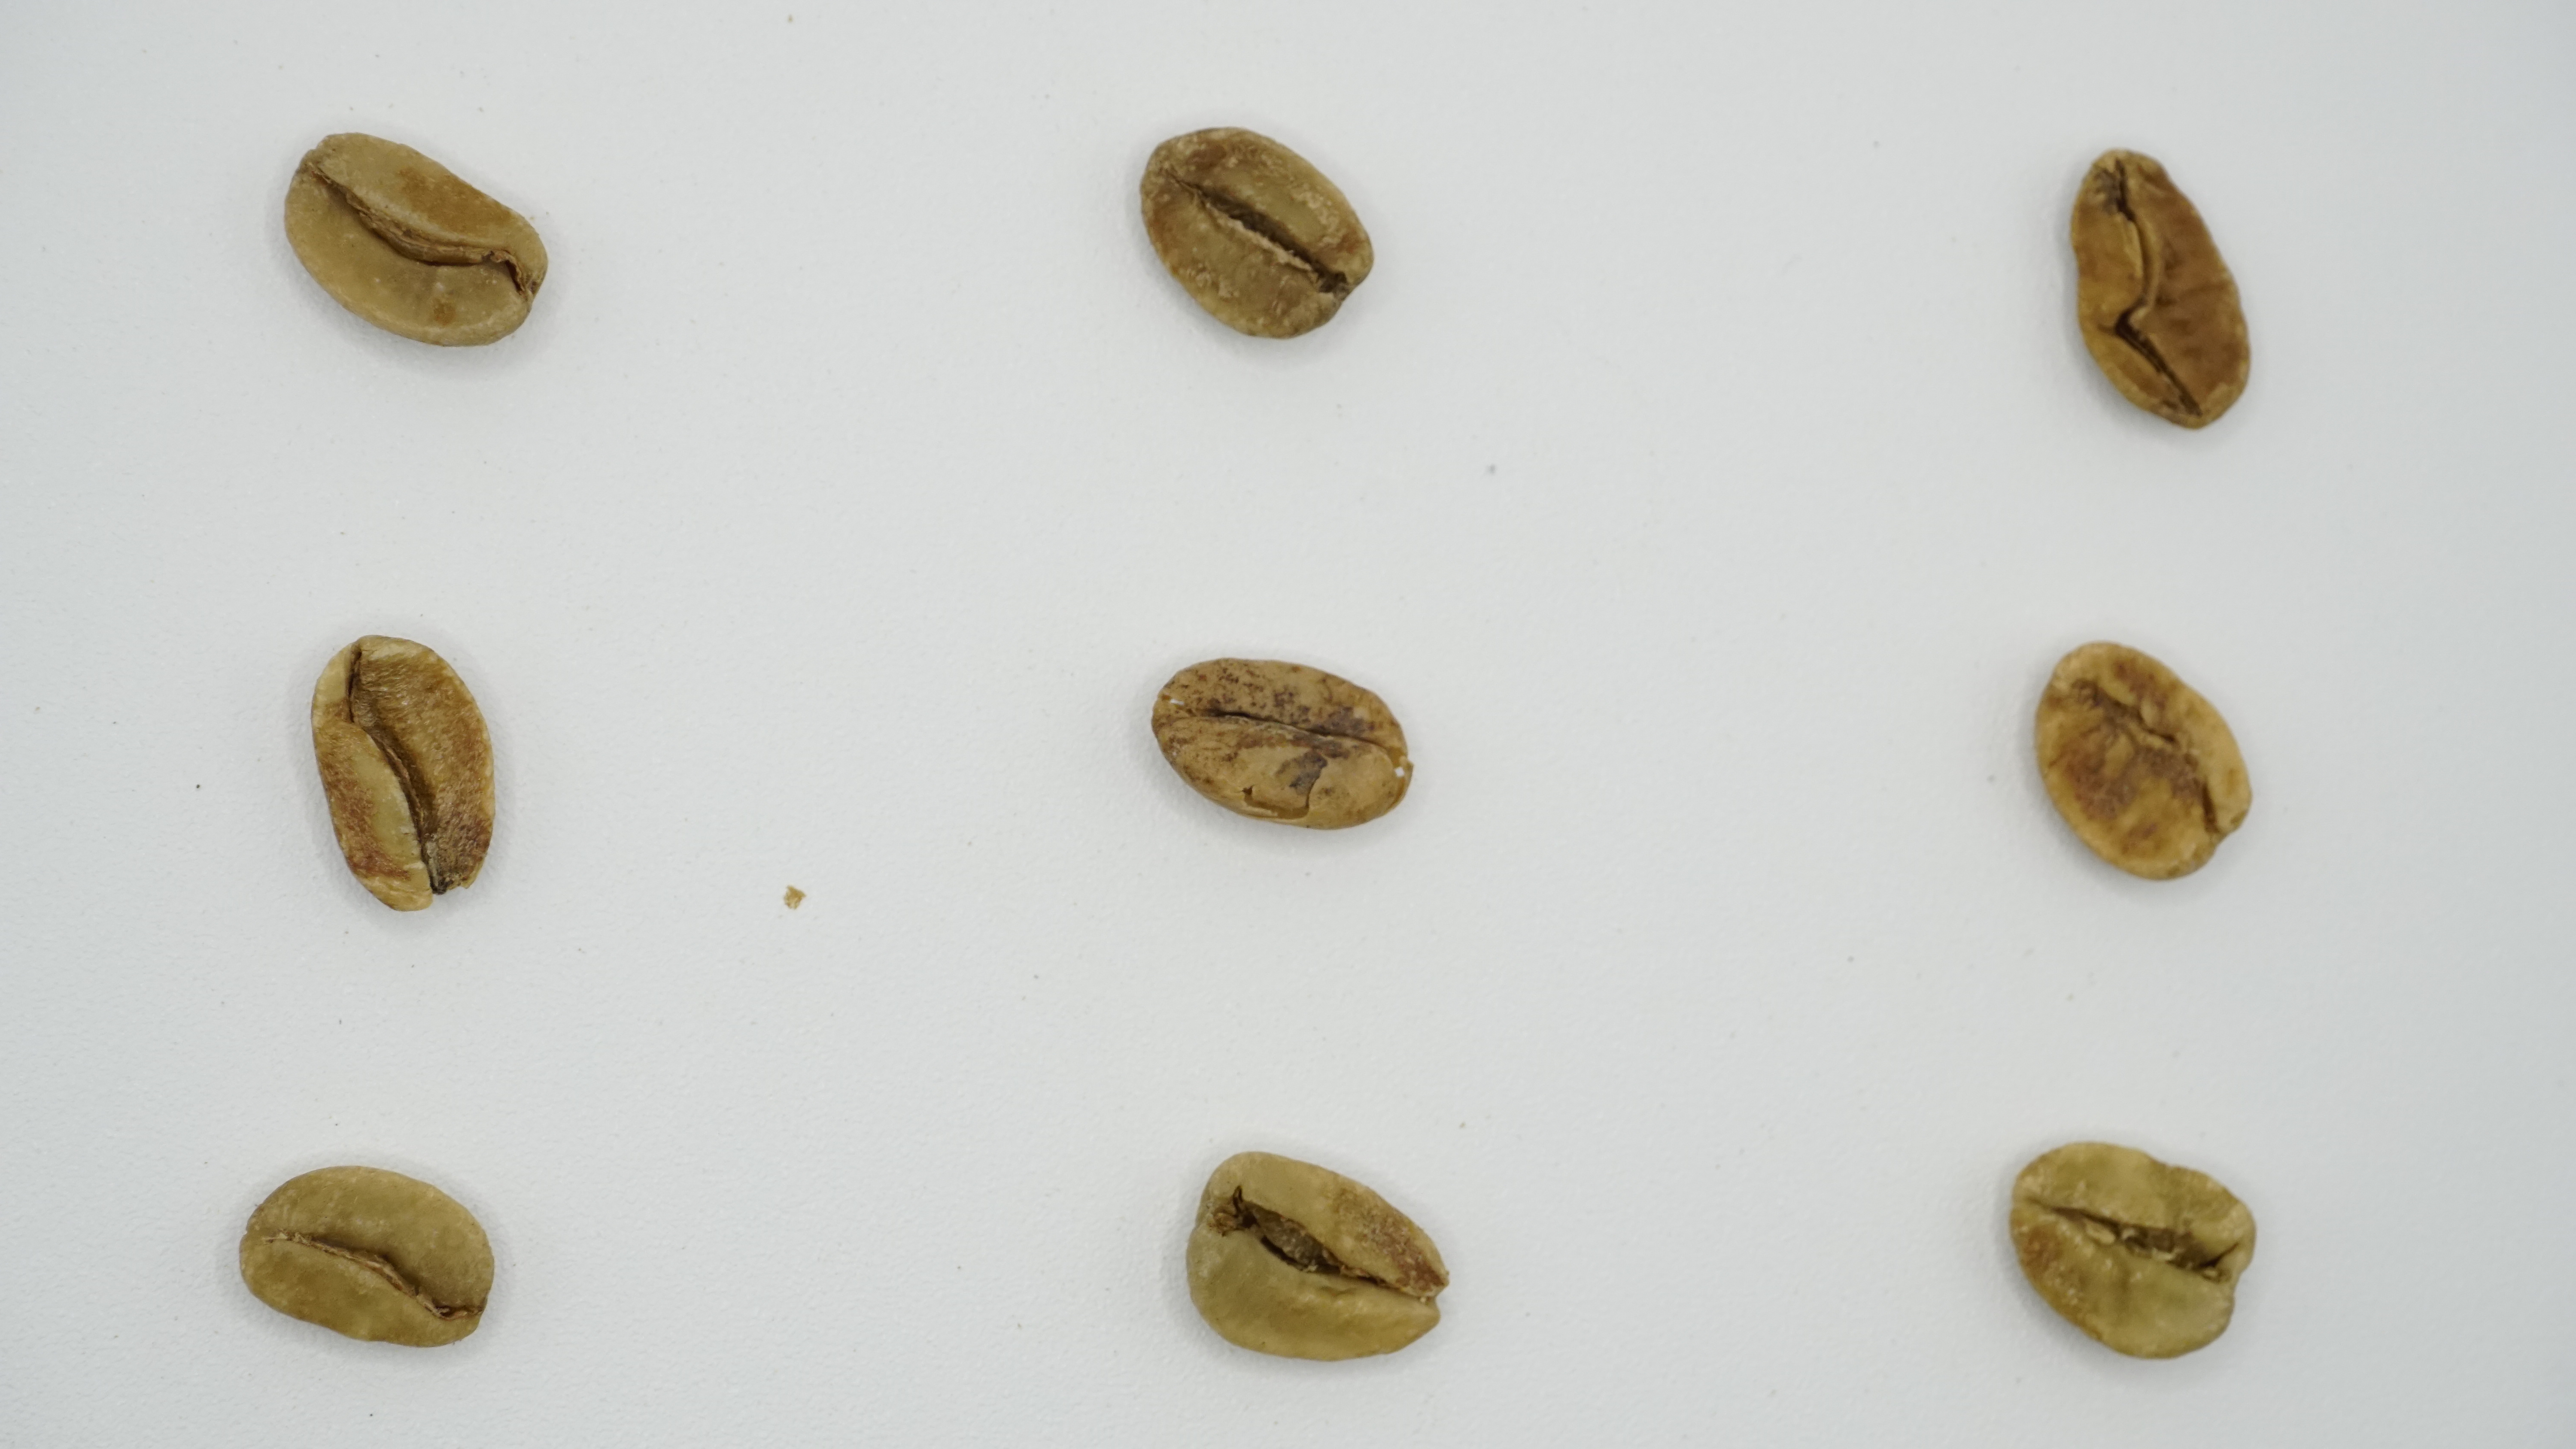
\includegraphics[width=0.3\textwidth]{ch5/1st-Iteration-Table/Sour.JPG} \\
		\textbf{Insect Damage}  & \textbf{Sour} \\[6pt]
	\end{tabular}
	\caption{Sample Images from the First Iteration of Dataset Collection}
\end{figure}


The first iteration of data collection utilized a Sony A6300 camera with its Kit Lens, set at 1/200 Shutter Speed, 1000 ISO, and a Distance of 50mm. The beans were captured in batches of nine, carefully arranged within the camera's field of view following the rule of thirds. The rule of thirds is a photographic composition principle where an image is divided into a 3x3 grid, creating nine equal grid lines to create balance to the photo. By aligning the coffee beans with the rule of thirds, the group ensured a structured and even distribution of the beans within the frame. This setup also made it easier to automate the cropping process, as the predefined positions of the beans allowed a Python script to accurately extract individual images.

\subsection{Second Iteration of Dataset Collection}
\begin{figure}[H]
	\centering
	\begin{tabular}{cc}
		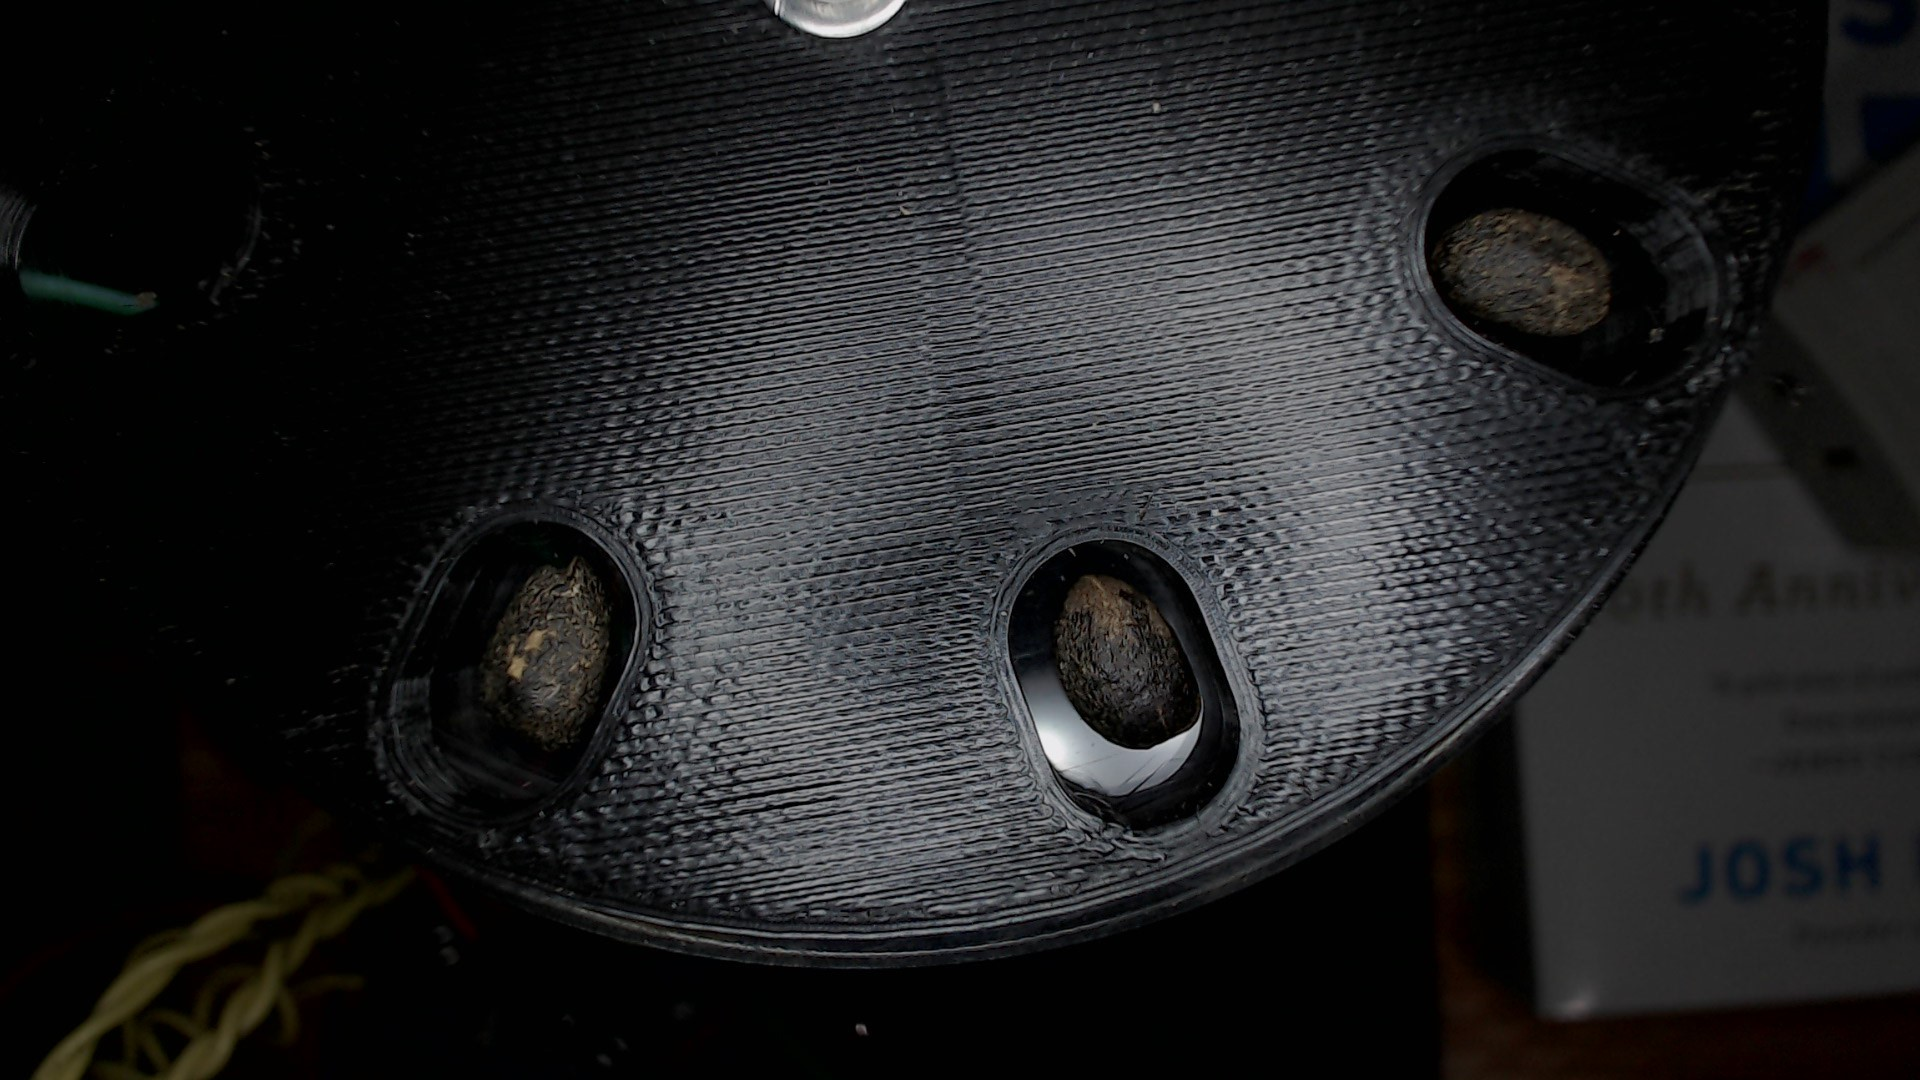
\includegraphics[width=0.3\textwidth]{ch5/2nd-Iteration-Table/Black.jpg} &
		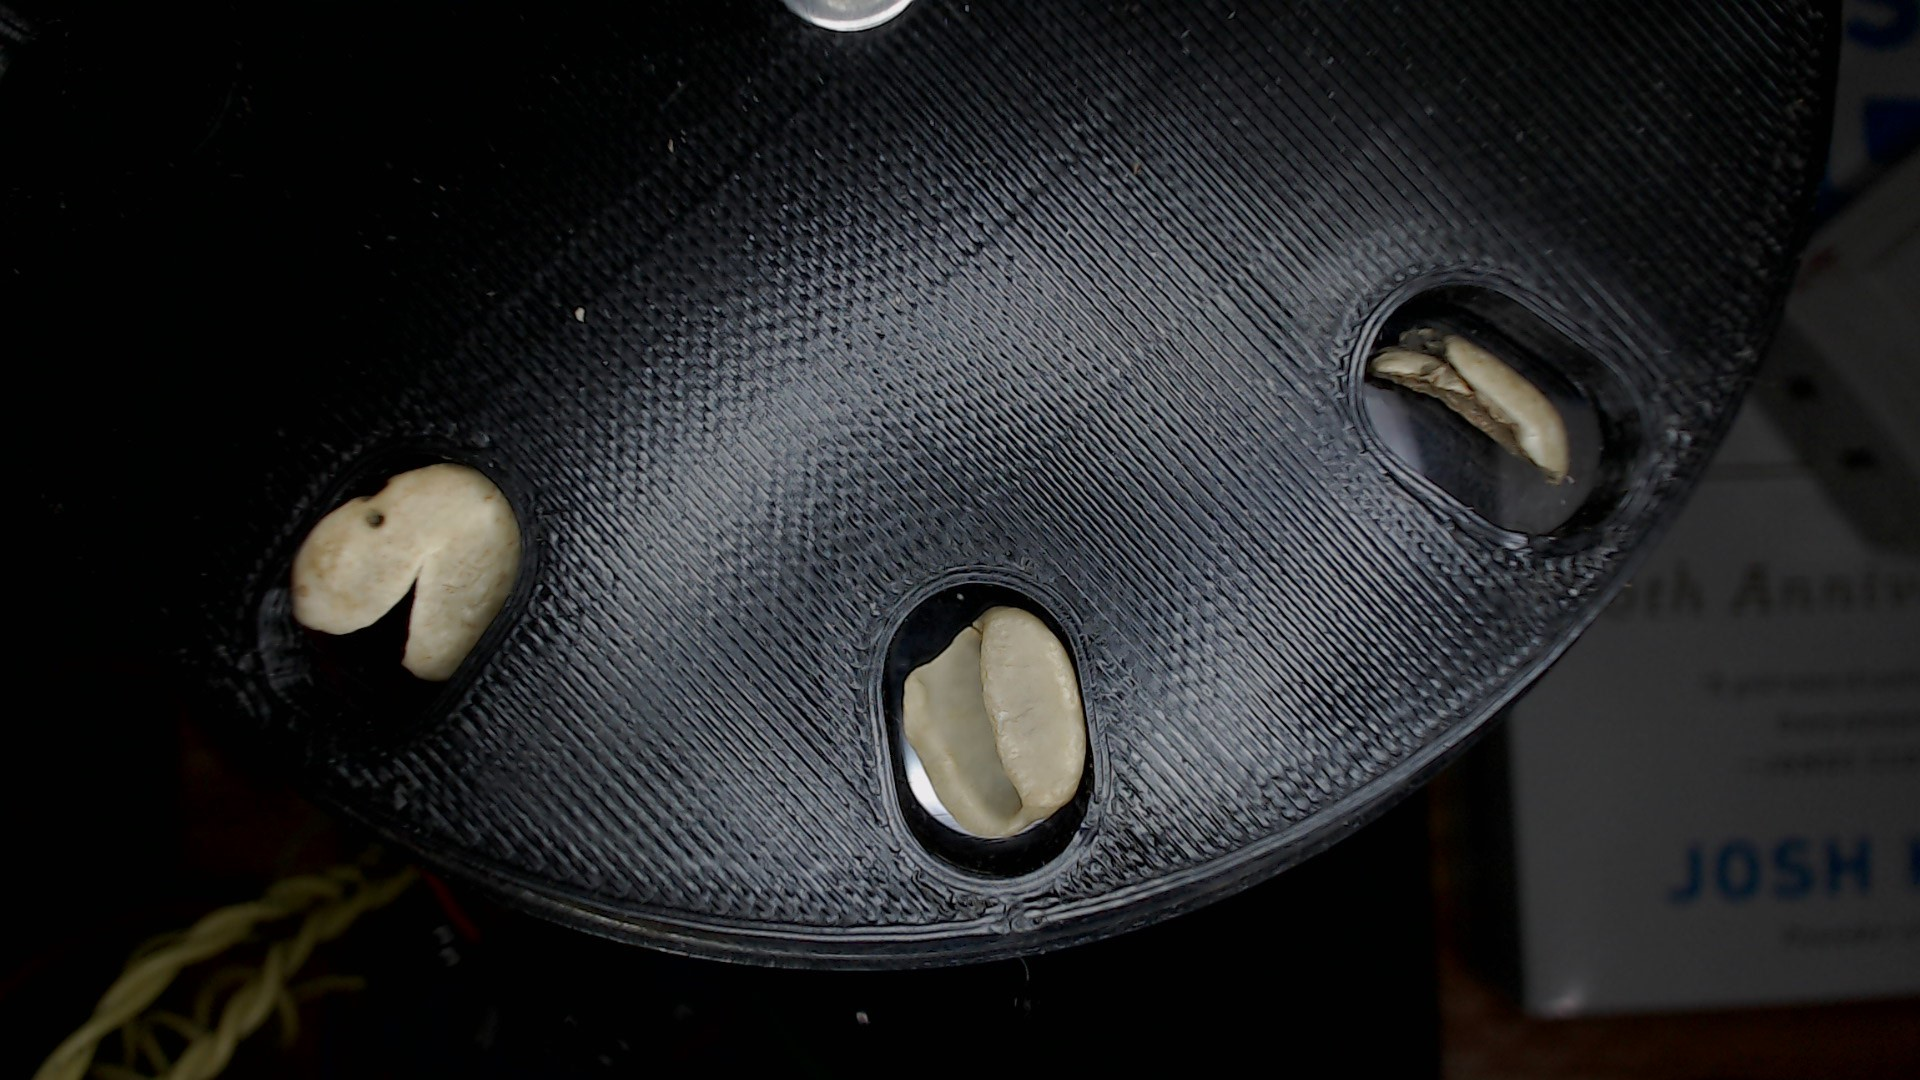
\includegraphics[width=0.3\textwidth]{ch5/2nd-Iteration-Table/Broken.jpg} \\
		\textbf{Black}  & \textbf{Broken} \\[6pt]
	\end{tabular}
	\begin{tabular}{cc}
		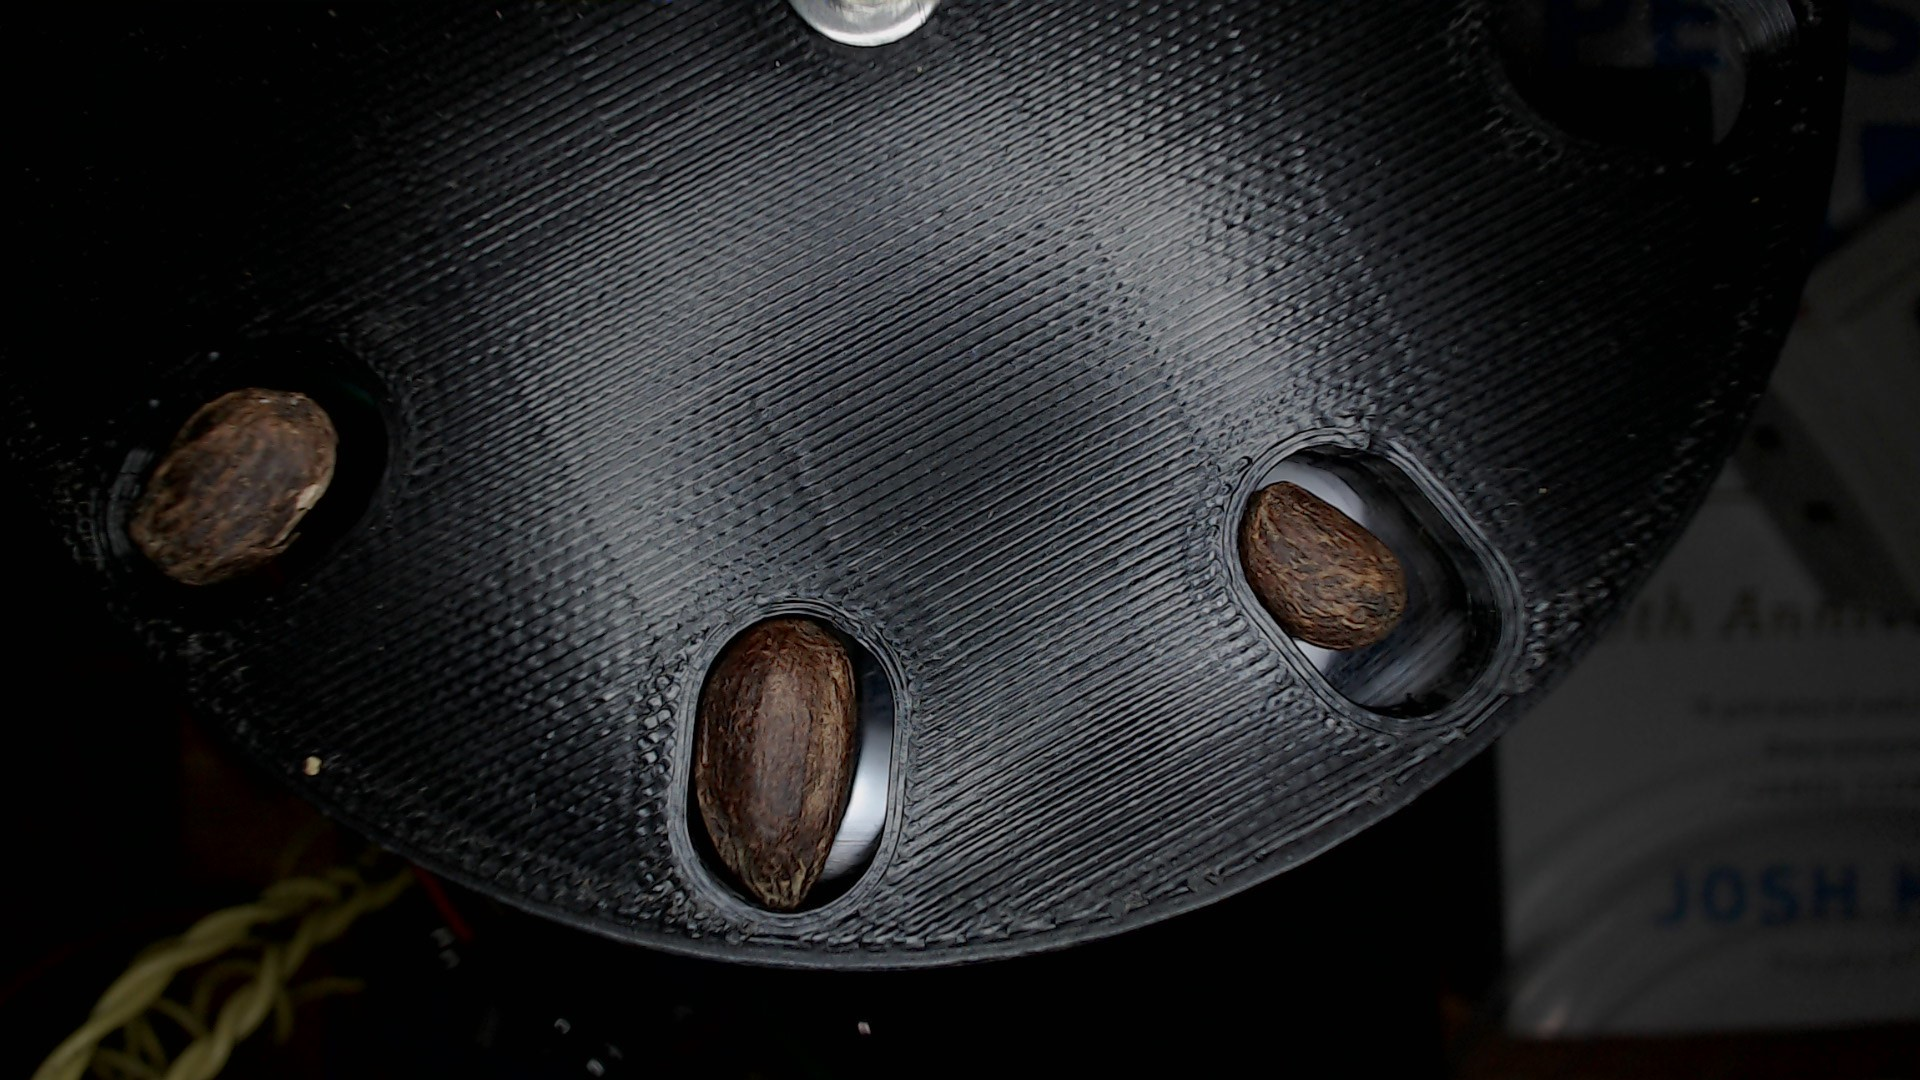
\includegraphics[width=0.3\textwidth]{ch5/2nd-Iteration-Table/DriedCherry.jpg} &
		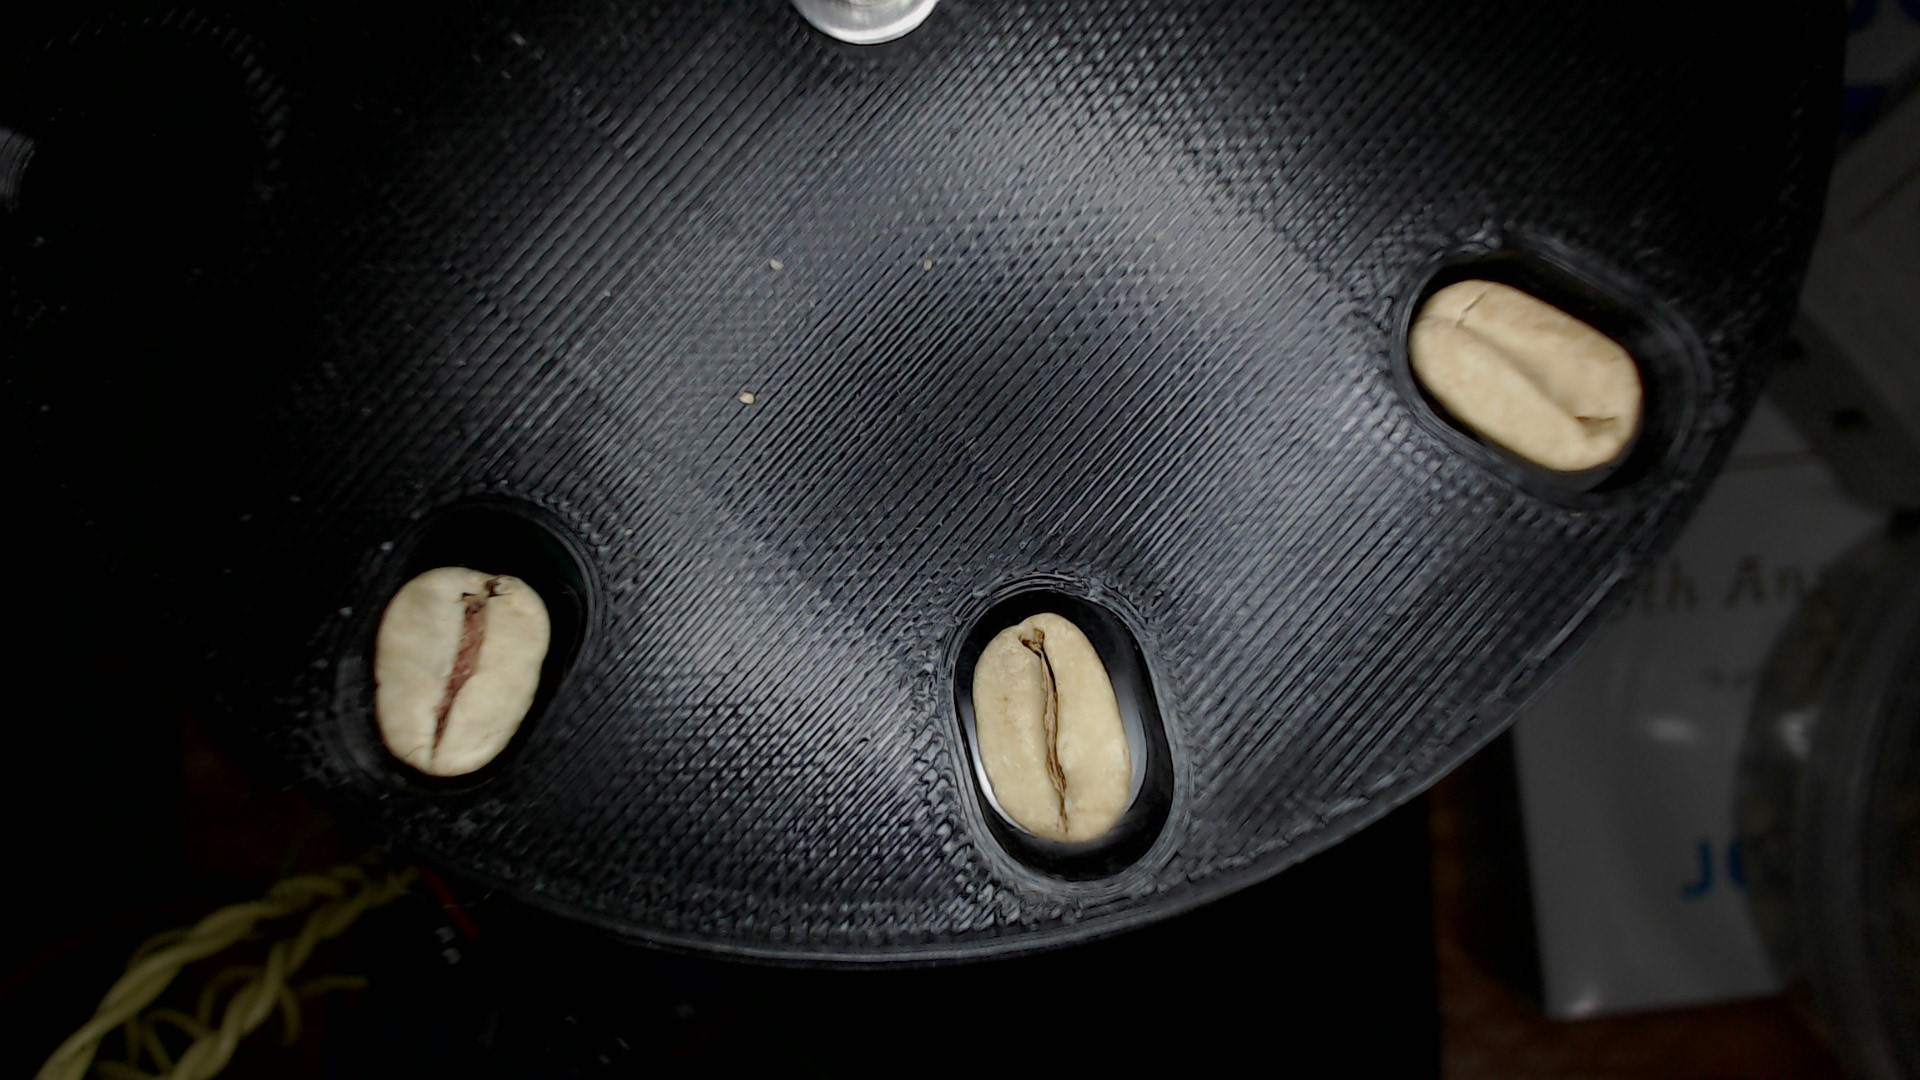
\includegraphics[width=0.3\textwidth]{ch5/2nd-Iteration-Table/Floater.jpg} \\
		\textbf{Dried Cherry}  & \textbf{Floater} \\[6pt]
	\end{tabular}
	\begin{tabular}{cc}
		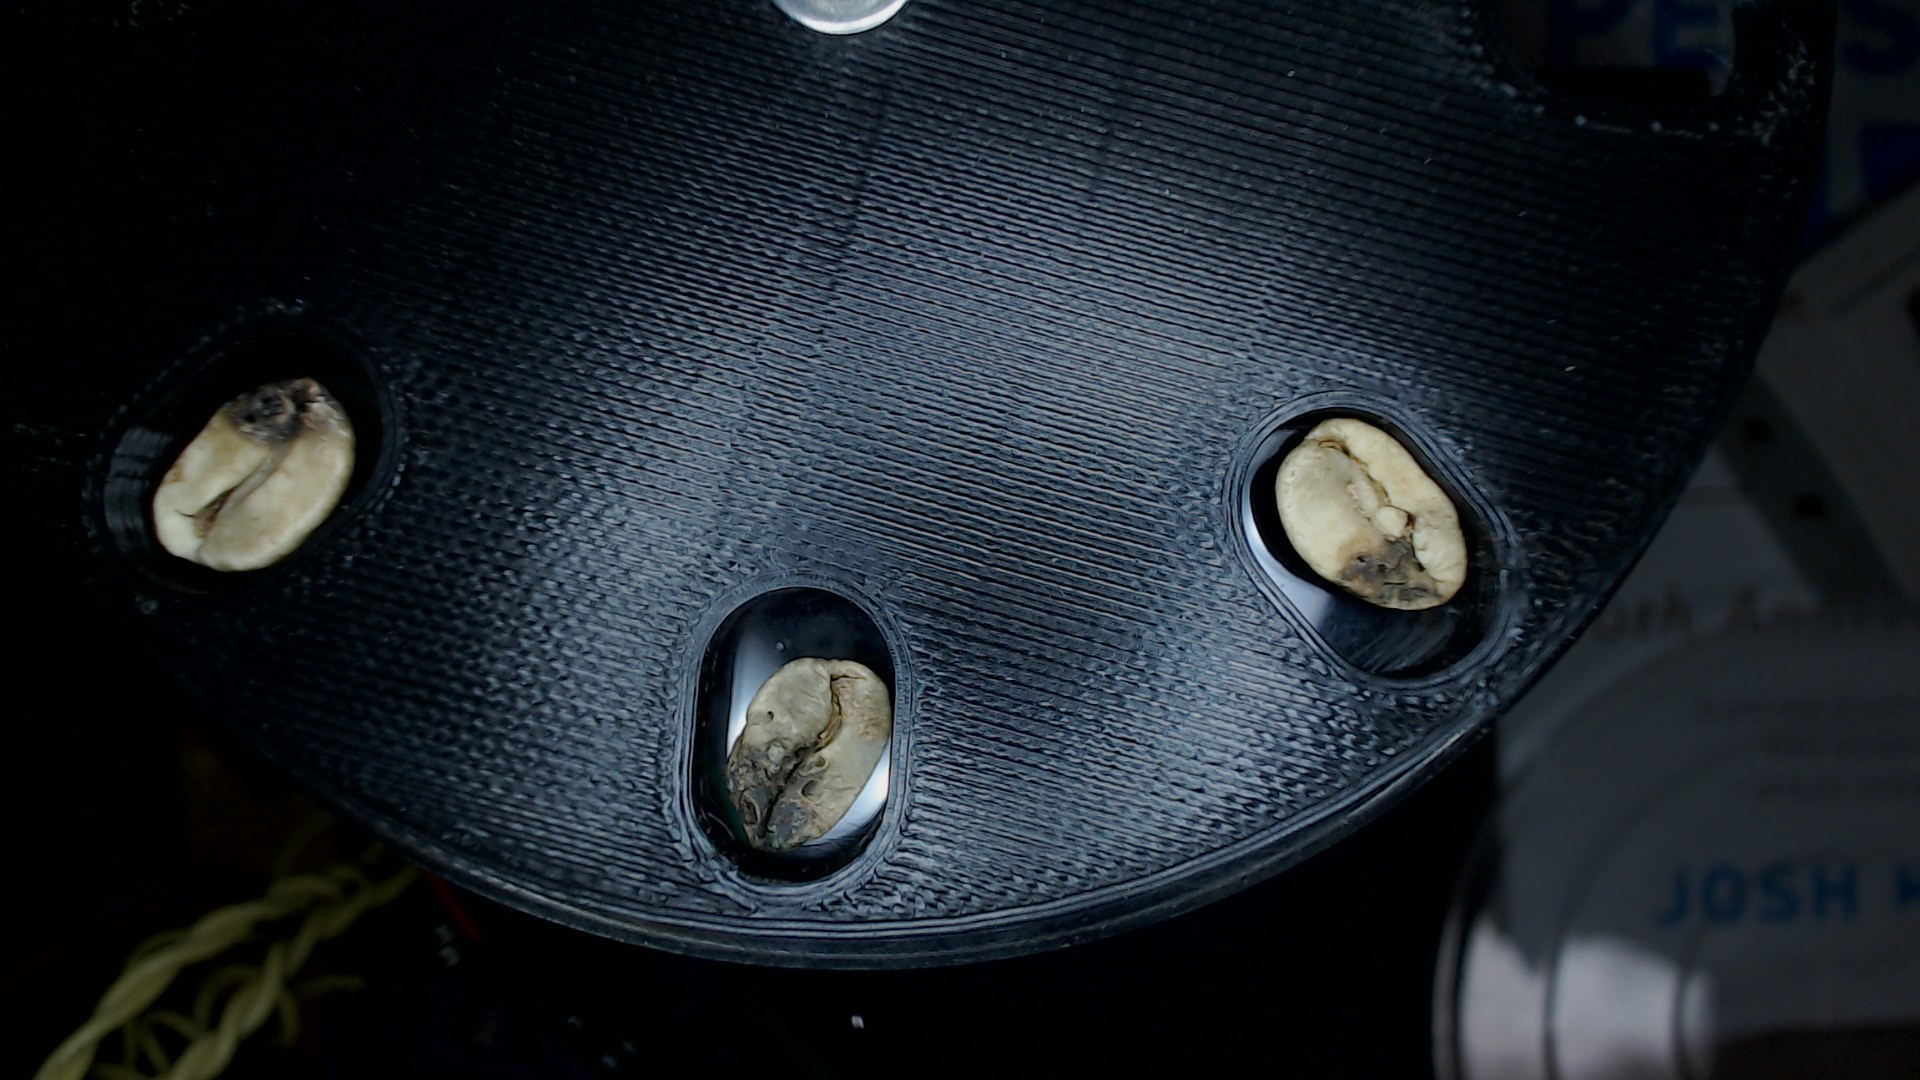
\includegraphics[width=0.3\textwidth]{ch5/2nd-Iteration-Table/FungusDamage.jpg} &
		\includegraphics[width=0.3\textwidth]{ch5/2nd-Iteration-Table/Good.jpg} \\
		\textbf{Fungus Damage}  & \textbf{Good} \\[6pt]
	\end{tabular}
	\begin{tabular}{cc}
		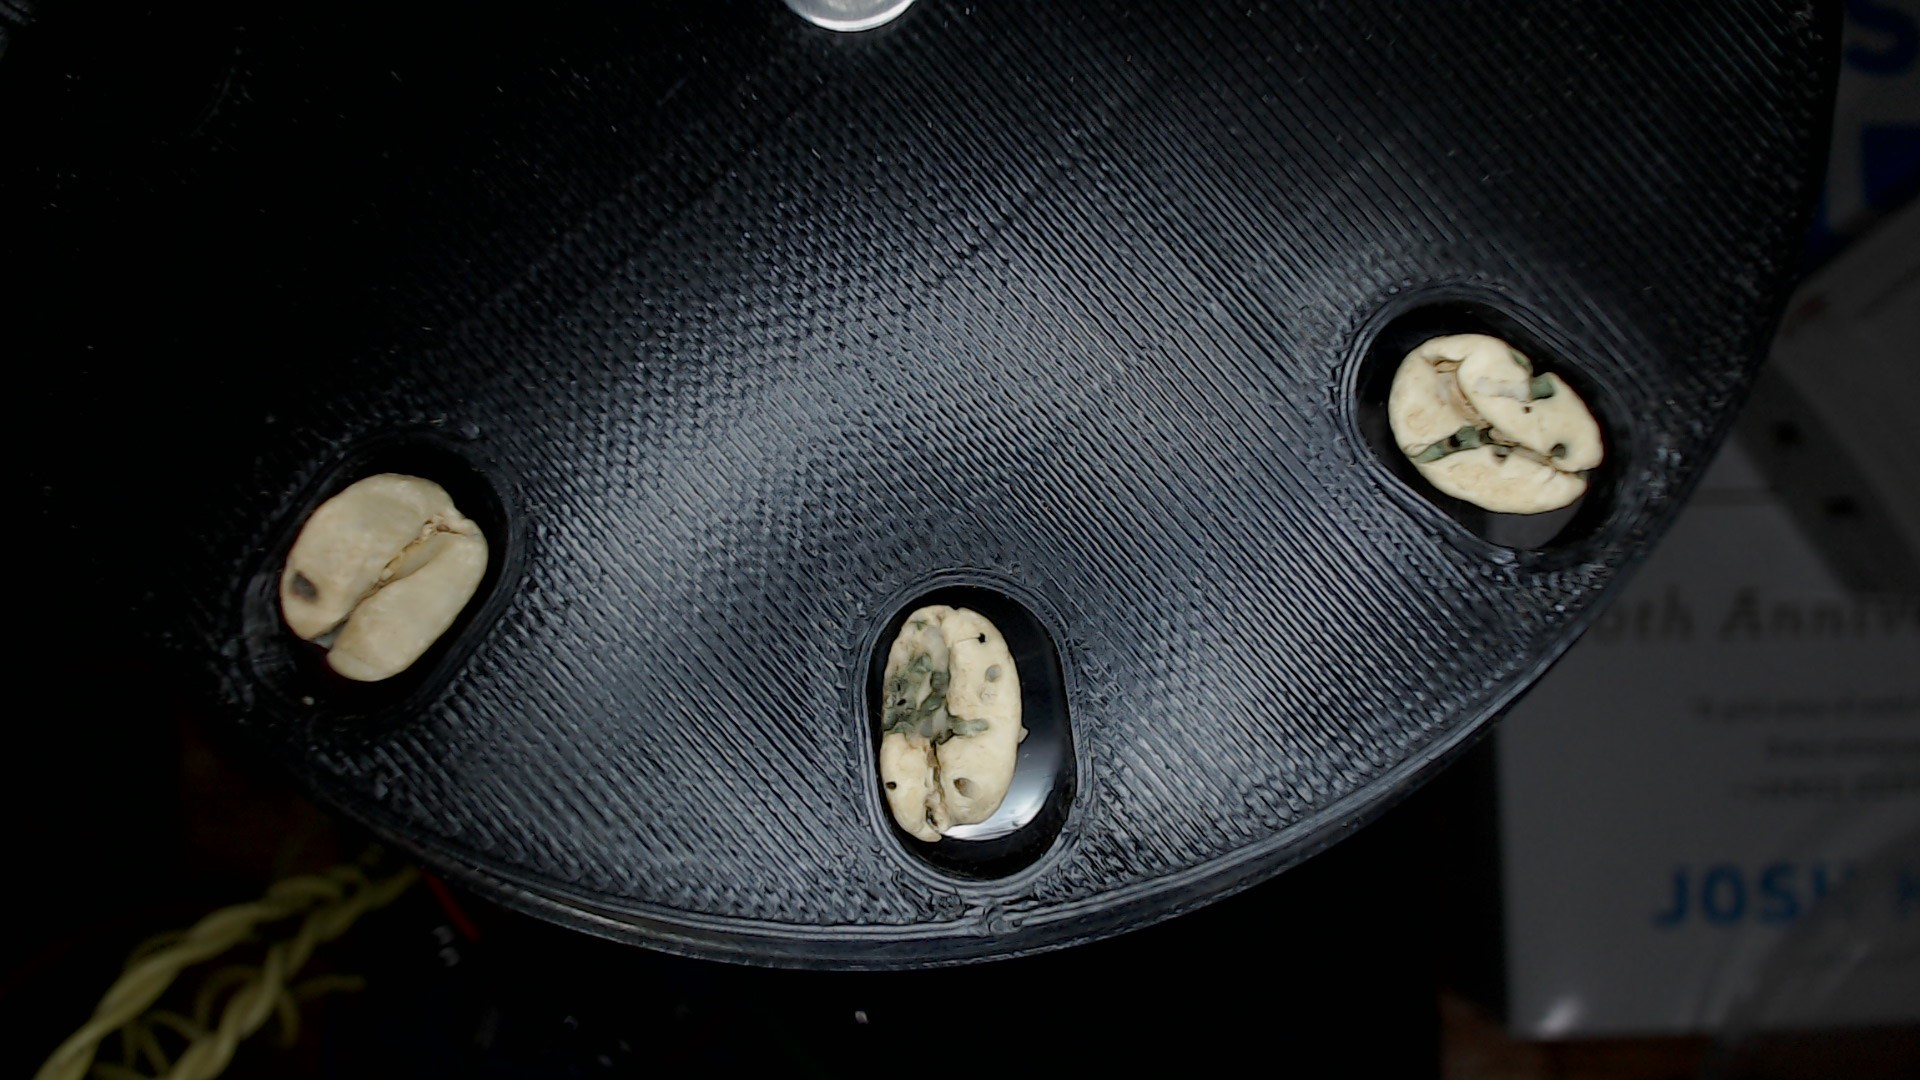
\includegraphics[width=0.3\textwidth]{ch5/2nd-Iteration-Table/InsectDamage.jpg} &
		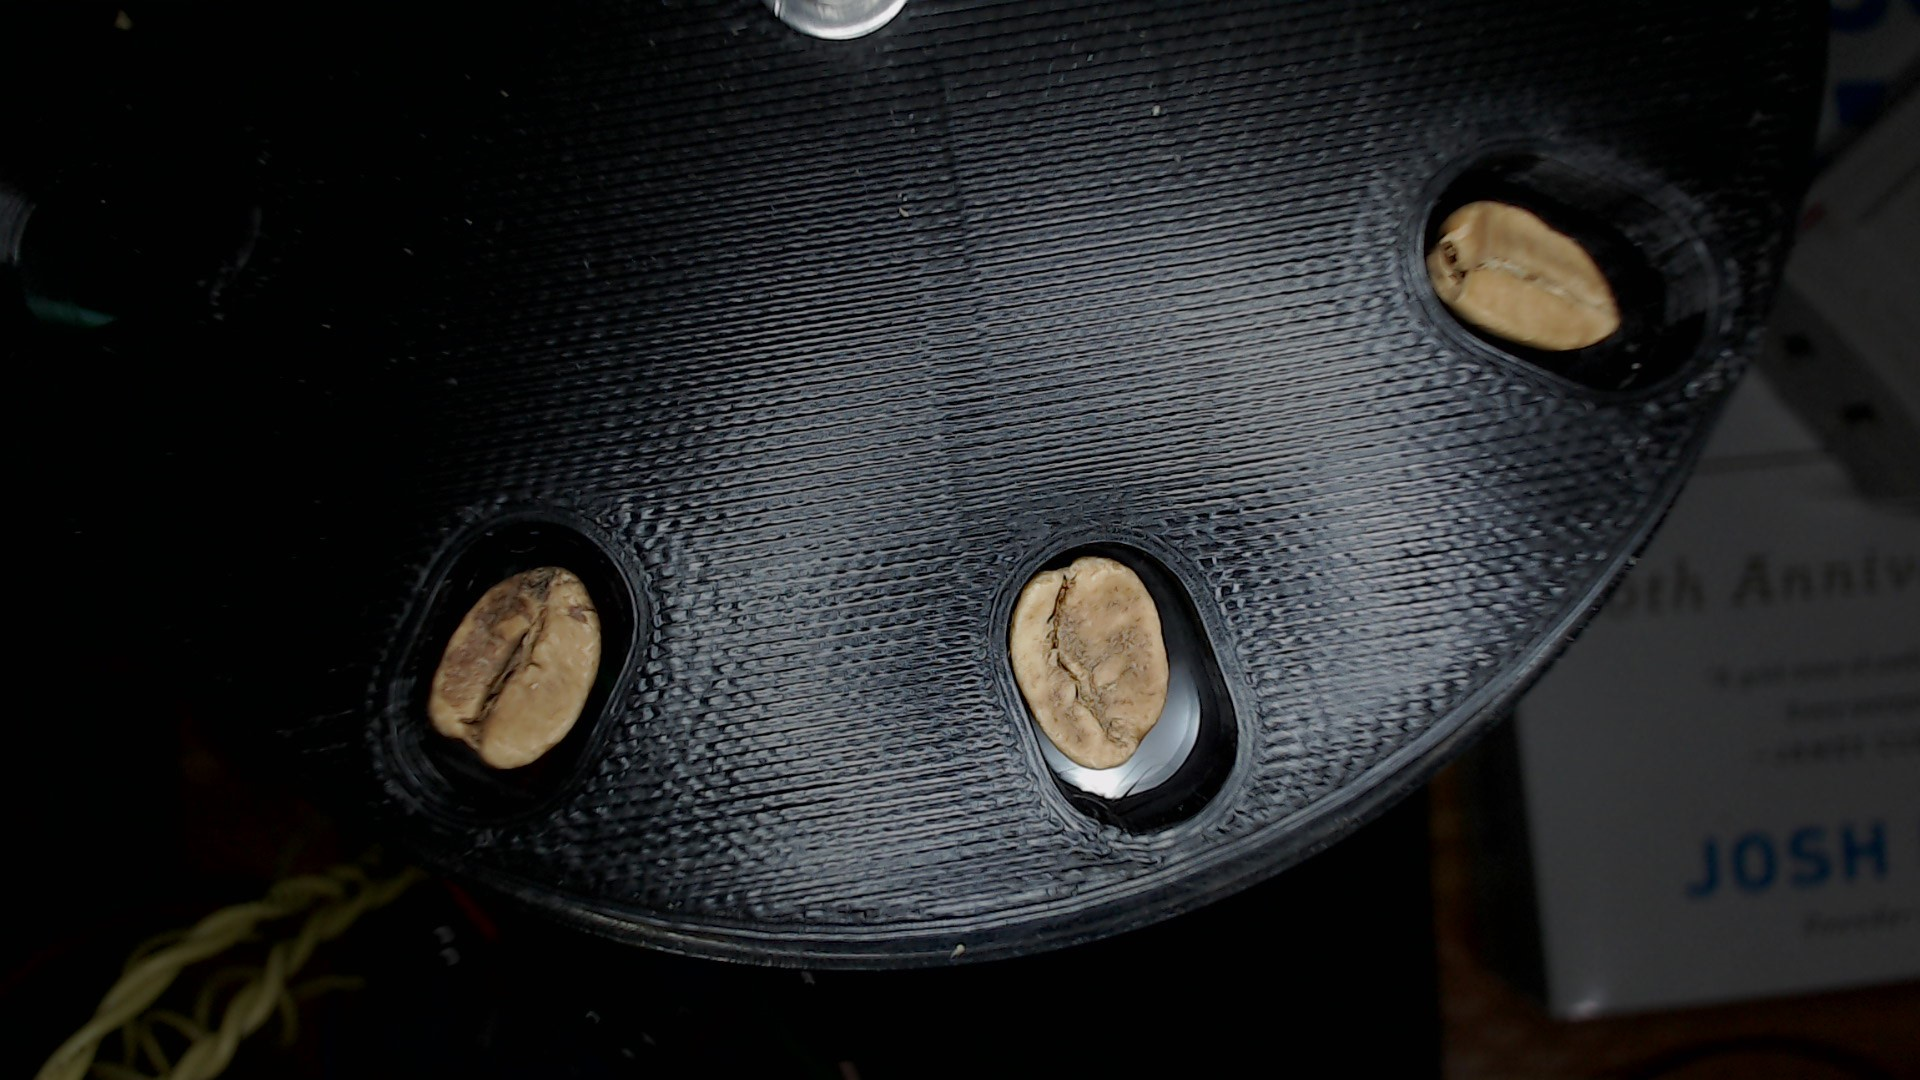
\includegraphics[width=0.3\textwidth]{ch5/2nd-Iteration-Table/Sour.jpg} \\
		\textbf{Insect Damage}  & \textbf{Sour} \\[6pt]
	\end{tabular}
	\caption{Sample Images from the Second Iteration of Dataset Collection}
\end{figure}

The second iteration focused on real-world implementation, using the system's built-in webcam to capture images directly from the inspection tray. This setup represents the ideal condition, as it replicates the actual environment where the model will operate. The images captured in this iteration directly reflect what the system will process in a practical application, allowing for better generalization and real-time adaptability.

\section{Dataset Preprocessing}
\label{sec:dataset_prep}
\subsection{Dataset Splitting}

The dataset is divided into train, validation, and test sets in a 70-20-10 ratio. The training dataset will be used for model learning, which allows it to identify patterns in the image. The validation set is used to assess the model’s performance and fine-tune the parameters of the model during training. This is an iterative process wherein the model learns from the training data and is then evaluated on and fine-tuned on the validation dataset. Finally, the test set is used for evaluating the model’s final performance, assessing its ability to generalize to new data.

\subsection{Image Annotation}

Roboflow Annotate was used to label images of coffee beans. The platform was used for two separate datasets: one for the detection model, the other for the classification model. In the detection dataset, bounding boxes were drawn around individual coffee beans and labeled accordingly. For the classification dataset, the trained detection model was used to crop individual coffee beans from the raw dataset, which were the categorized into the eight different classifications. Roboflow was chosen for its ability to store datasets in the cloud and its support for different annotation formats, such as COCO and YOLO, ensuring compatibility with different deep learning models during experimentation.

\subsection{Dataset Augmentation Techniques}

Data augmentation techniques were applied using Roboflow’s tools to improve the model generalization. Different augmentations such as rotation, flipping, blur, brightness and contrast adjustment, and noise were used to simulate variations, which helps prevent overfitting and improve the model’s ability to identify defects in different lighting conditions and orientations.

\section{Density Analysis}
\label{sec:density_analysis}

\subsection{Density Estimation}
To estimate the volume of the bean through computer vision, bounding boxes are implemented to first determine the area to be used for the volume estimation. Using the bounding boxes to determine a pixel value for the green coffee bean, this will be used to scale the image gathered from pixels to their estimated length and width. 

Through the estimated length and width gathered, this is compared to the actual length and width of the green coffee bean to compare both parameters. Through this, it is possible to estimate the volume of the green coffee bean through computer vision. The formula for triaxial ellipsoid is used to determine the volume of the green coffee bean.

The total volume of the batch of beans was measured by the water displacement technique, a commonly used method to measure the volume of solids that are irregularly shaped. The beans were fully immersed in a water-filled graduated cylinder, and the rise in water level was measured. The volume of water displaced is equivalent to the combined volume of the batch of beans, measured in cubic centimeters (cm$^3$).

Comparing the volume measured through water displacement and the volume gathered by computing for the volume using the triaxial ellipsoid volume formula, the volumes differ by -6.52\% up to +6.67\%, with most errors within the $\pm$5\%. This indicates that the model used to determine the volume of the green coffee bean is consistent with the ground-truth measurements. 


The overall weight of the beans was determined by a high-precision digital scale (at least to 0.001 g resolution). Both the mass and volume are known, and the batch density may be calculated through the use of the standard formula for density:

\[
\text{Batch Density} = \frac{\text{Total Mass of Beans} \, (g)}{\text{Total Volume Displaced} \, (cm^3)}
\]

Obtaining the volume through computer vision, and obtaining the weight of the bean through the precision scale, an estimated density is obtained that will be used to sort out the less dense from th dense beans. 

\subsection{Density Threshold Calibration}
\label{sec:density_threshold_calibration}
Setting the threshold for bean density is crucial for the stage 2 sorting of the system, which involves measuring the density of each bean. In order to set a threshold for density-based classification, a calibration batch of Good quality coffee beans was chosen. The beans were confirmed to be free of defects and representative of typical specialty-grade coffee by the farmer. The threshold density was calculated by determining the average density of this batch through direct measurements of mass and volume.

The computed average density served as the threshold value in the system. During automated classification, individual bean density is calculated using estimated volume (from image analysis) and actual weight (from the precision scale via RS232 communication). Beans with a density lower than the threshold are classified as less dense, while those meeting or exceeding the threshold are considered dense, indicating higher quality.

\section{Model Training}

\subsection{Image Detection Models}

The object detection model identifies and isolates the coffee beans from the background. For this task, different models were explored:

\begin{enumerate}
	\item \textbf{RF-DETR}
	 
	A transformer-based object detection model that eliminates the need for anchor boxes, improving small object detection.

	\item \textbf{YOLOv11}
	
	A CNN-based YOLO variant that incorporates the C3k2 block, SPPF, and C2PSA components to enhance feature extraction and detection accuracy.

	\item \textbf{YOLOv12}
	
	The latest YOLO version and attention-centric model that integrates transformer-based components to enhance performance while maintaining real-time efficiency.
\end{enumerate}

\subsection{Image Classification Models}
Following detection, each identified coffee bean was cropped and classified based on its defect type. The classification models used included:

\begin{enumerate}
	\item \textbf{EfficientNetV2}
	 
	A convolutional neural network (CNN) designed for high efficiency and accuracy, balancing computational cost and performance.
	
	\item \textbf{YOLOv8}
	
	A lightweight yet highly accurate model that supports both object detection and classification, making it suitable for real-time applications.

	\item \textbf{YOLOv11}
	
	A classification-specific adaptation of YOLOv11, leveraging enhanced feature extraction techniques for defect recognition.
	
	\item \textbf{YOLOv12}
	
	A classification variant of YOLOv12, incorporating advanced attention mechanisms to improve accuracy.

	\item \textbf{Vision Transformer (ViT)}

	The Vision Transformer (ViT) processes images as sequences of tokens for classification \cite{Dosovitskiy_Beyer_Kolesnikov_Weissenborn_Zhai_Unterthiner_Dehghani_Minderer_Heigold_Gelly_2021}. A learnable “class token” is added to the sequence to support classification. Through the attention mechanism, it captures dependencies between image tokens. The encoder is composed of repeated multi-head self-attention and feedforward layers, with self-attention computing weighted sums of sequence elements.
\end{enumerate}

\subsection{Bean Classification Logic}
To ensure proper classification, conditions are set based on how the top and bottom-side of the beans are categorized. For a bean to be labeled Good, both sides need to be classified as such. Similarly, Dried Cherry requires both sides to be classified as such, since Black beans can resemble Dried Cherry on its outer side. Moreover, both sides must be classified as Fungus Damage to be considered as such. If one side is classified as Black and the other Dried Cherry, or both are Black, then it will be labeled as Black.  The rest of the defect types are sufficient for single-side detection, as seen in Table \ref{tab:pseudocode_classification}.


\begin{table}[H]
	\caption{Classification Algorithm for Coffee Beans}
	\label{tab:pseudocode_classification}
	{\footnotesize
	\begin{tabular}{lll}
	\hline
	\hline
	{\bfseries Input(s):} & & \\
	$top\_class$ & : & classification result from top camera; $top\_class \in \mathbb{Z}^{+}$ \\
	$bottom\_class$ & : & classification result from bottom camera; $bottom\_class \in \mathbb{Z}^{+}$ \\
	\hline
	{\bfseries Output(s):} & & \\
	$class$ & : & final bean classification (Good, Defective, or specific defect) \\
	\hline
	\hline
	\\
	\end{tabular}
	}
	\begin{algorithmic}[1]
	{\footnotesize
		\IF{$top\_class = 5 \wedge bottom\_class = 5$}
			\STATE $class \Leftarrow$ ``Good''
		\ELSIF{$top\_class = 2 \wedge bottom\_class = 2$}
			\STATE $class \Leftarrow$ ``Dried Cherry''
		\ELSIF{$(top\_class = 0 \wedge bottom\_class = 0) \vee (top\_class = 0 \wedge bottom\_class = 2) \vee (top\_class = 2 \wedge bottom\_class = 0)$}
			\STATE $class \Leftarrow$ ``Black''
		\ELSIF{$top\_class = 4 \wedge bottom\_class = 4$}
			\STATE $class \Leftarrow$ ``Fungus Damage''
		\ELSIF{$top\_class = 6 \wedge bottom\_class = 6$}
			\STATE $class \Leftarrow$ ``Insect Damage''
		\ELSIF{$top\_class = 1 \vee bottom\_class = 1$}
			\STATE $class \Leftarrow$ ``Broken''
		\ELSIF{$top\_class = 7 \vee bottom\_class = 7$}
			\STATE $class \Leftarrow$ ``Sour''
		\ELSIF{$top\_class = 3 \vee bottom\_class = 3$}
			\STATE $class \Leftarrow$ ``Floater''
		\ELSE
			\STATE $class \Leftarrow$ ``Defective''
		\ENDIF
		\RETURN $class$
	}	
	\end{algorithmic}
\end{table}


\subsection{Model Evaluation}
Each trained model will be tested on the system, with a predetermined set of beans. The results from this test are analyzed by using a confusion matrix, providing a detailed breakdown of the model’s performance for each category. The confusion matrix provides a way to interpret classification results by defining the following parameters:
\begin{itemize}
    \item \textbf{True Positives (TP)} - The number of correctly classified instances for a specific defect type.
    \item \textbf{False Positives (FP)} - The number of times a different category was incorrectly classified as this defect type.
    \item \textbf{True Negatives (TN)} - All correctly classified instances excluding the defect category in question.
    \item \textbf{False Negatives (FN)} - The number of times this defect type was classified as something else.
\end{itemize}

Through these parameters, key performance metrics such as accuracy, precision, recall, and F1-score were computed to evaluate the system’s performance in different classifications as shown below. This test will assist in determining what types of defects the system correctly classifies and which types might need improvements in image preprocessing, dataset expansion, or optimization of the machine learning model. The outcome will be applied to optimize the sorting algorithm for minimal misclassifications to ensure greater reliability in real-world defect detection.

\begin{enumerate}
	\item \textbf{Accuracy} measures overall correctness of the classification model
	\begin{equation}
	Accuracy = \frac{TP + TN}{TP + TN + FP + FN}
	\end{equation}

	\item \textbf{Precision} measures how many of the predicted positive classifications were actually correct
	\begin{equation}
	Precision = \frac{TP}{TP + FP}
	\end{equation}

	\item \textbf{Recall} evaluates how well the model identifies actual positive cases
	\begin{equation}
	Recall = \frac{TP}{TP + FN}
\end{equation}
	
	\item \textbf{F1-score} represents the harmonic mean of precision and recall
\begin{equation}
	F1\text{-}Score = 2 \times \frac{Precision \times Recall}{Precision + Recall}
	\end{equation}
\end{enumerate}

\subsection{Model Benchmarking and Selection}
A total of 5 models were trained and tested within the actual system to determine the most effective one. These models trained and evaluated include EfficientNetV2, YOLOv8, YOLOv11, YOLOv12, and ViT. Each model was assessed using the defined performance metrics and compared accordingly. The model with the highest overall performance will be selected for deployment in the system.


\section{Hardware Development}
The hardware elements of the system, two-stage automated coffee bean sorter, are developed to provide effective and precise sorting using a mix of mechanical and electronic components. Each element is designed and tested to maximize the sorting process while providing system reliability.

\subsection{Screw Feeder}
\begin{figure}[H]
    \centering
    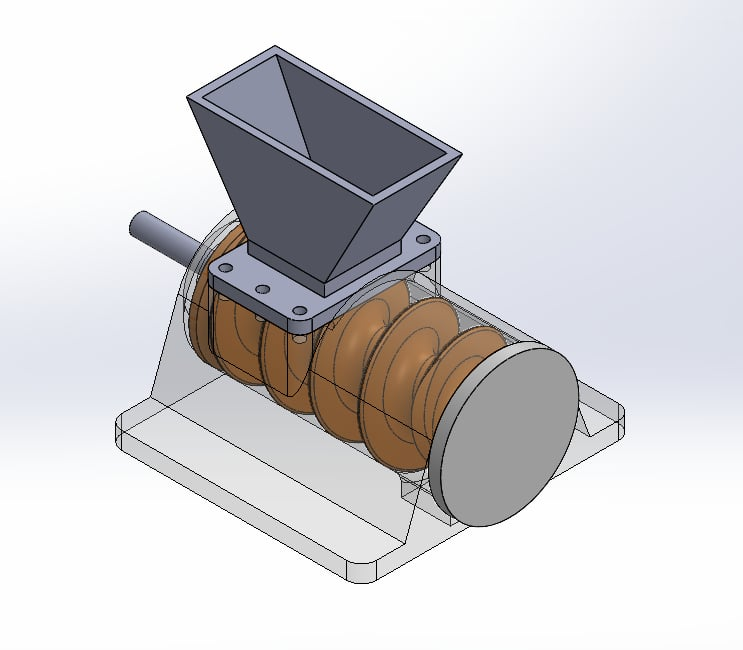
\includegraphics[width=9cm]{ch5/Screw_Feeder_Design.jpg}
    \caption{Screw Feeder 3D Design}
    \label{fig:screw_feeder}
\end{figure}
Screw feeder is the most essential of the devices as it governs the beans of coffee moving into the system. It operates mostly to deliver the beans consistently in terms of volume and ensures they do not bundle up and fall into the system in heavy masses, causing beans build up on the rotating conveyor table. The feeder is driven by a 12V DC motor, and the rotation speed is regulated using PWM. Through a constant and controlled flow, the screw feeder avoids clogging and provides a consistent input into the inspection tray, enhancing overall system performance. Figure \ref{fig:screw_feeder} shows the actual 3D model design of the screw feeder used in the system. 

\subsection{Rotating Conveyor Table}
\begin{figure}[H]
    \centering
    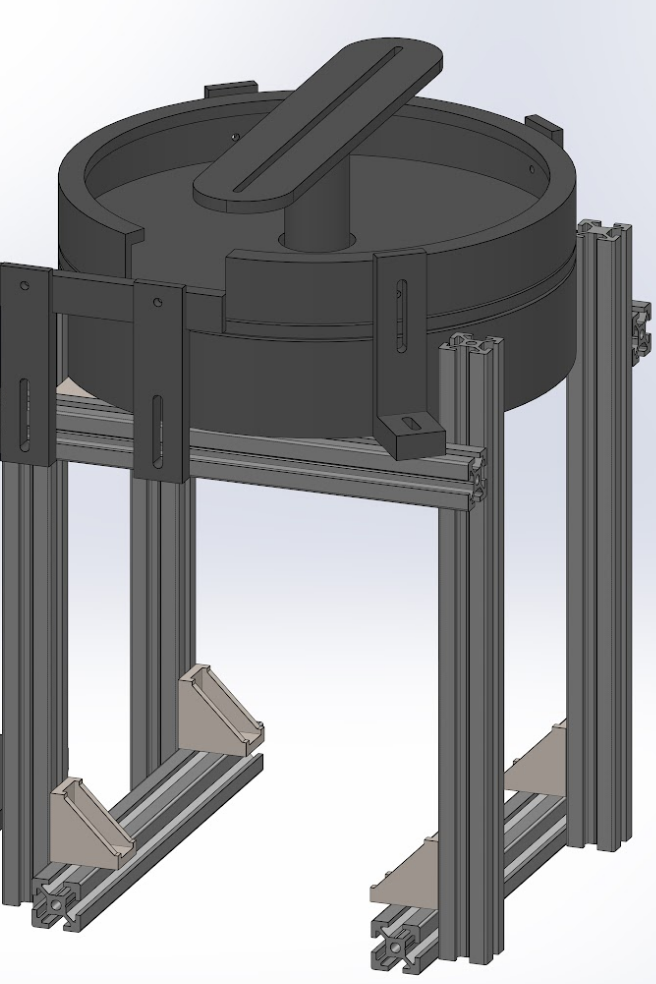
\includegraphics[width=7cm]{ch5/Rotating_Conveyor_Table_Design.png}
    \caption{Rotating Conveyor Table 3D Design}
    \label{fig:rotating_conveyor}
\end{figure}
The conveyor table, as shown in Figure \ref{fig:rotating_conveyor}, rotates to move the coffee beans from the feeding mechanism to the inspection tray. The table contains aluminum guides to linearly arrange the beans prior to dropping on the inspection tray. The conveyor is powered by a 12V DC motor, which offers consistent movement and regulated speed to avoid misalignment. By incorporating a turning mechanism, the conveyor guarantees beans are well oriented prior to inspection tray entry, minimizing classification errors due to faulty positioning.

\begin{figure}[H]
    \centering
    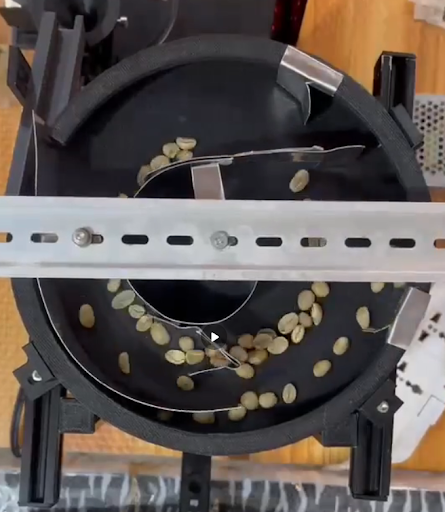
\includegraphics[width=9cm]{ch5/Rotating_Conveyor_Table_with_Aluminum_Guides.png}
    \caption{Rotating Conveyor Table with Aluminum Guides}
    \label{fig:rotating_conveyor_aluminum}
\end{figure}
As shown in Figure \ref{fig:rotating_conveyor_aluminum}, there are aluminum guides on the rotating conveyor table that ensures coffee beans to be linearly arranged. This linear arrangement of beans significantly helped the system to ensure that coffee beans are dropped onto the slide, which connects the conveyor table to the inspection try, in a one-by-one manner. In addition, the guides are also installed to keep the beans from accumulating in one area, which can cause the jamming of beans. The researchers tested the different motor speeds to observe the optimal settings that will not cause bean jamming and meet the minimum sorting speed of the system. However, while the aluminum guides are effective in arranging the beans linearly, it was hard to re-calibrate or adjust. Another problem was it was easy to be deformed whenever there was jamming of beans. Upon printing the model, the bearing of the rotating mechanism was also not robust enough to hold the motor in higher RPM. There are instances where the gearing mechanism between the motor and the conveyor table experiences jamming, resulting in the conveyor table temporarily ceasing rotation. This issue typically arises from misalignment or friction within the gear interface, which hinders the smooth transfer of torque from the motor to the conveyor table.


\begin{figure}[H]
    \centering
    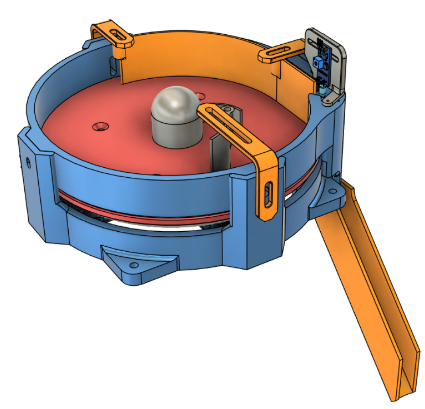
\includegraphics[width=9cm]{ch5/Revised_Rotating_Conveyor_Table.png}
    \caption{Revised Rotating Conveyor Table}
    \label{fig:revised_rotating_conveyor}
\end{figure}
Figure \ref{fig:revised_rotating_conveyor} shows the re-designed conveyor table. In this revision, calibration of the guides was easier since it can be moved by only loosening the screws. To avoid the issue caused by the misalignment within the gear of the previous rotating table mechanism, the researchers opted to revise the design. The new iteration of the rotating conveyor table was redesigned using a Lazy Susan bearing. In this modification, smoother rotation was observed. 

\begin{figure}[H]
    \centering
    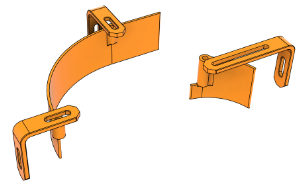
\includegraphics[width=9cm]{ch5/3D-Printed_Guides.png}
    \caption{3D Printed Guides}
    \label{fig:3d_printed_guides}
\end{figure}
In addition, the previously aluminum guides were replaced with 3D-printed guides that were screwed onto the table walls. The revised design allowed for easier calibration, as the guides could be repositioned simply by loosening the screws, enabling more precise alignment of beans. 

\begin{figure}[H]
    \centering
    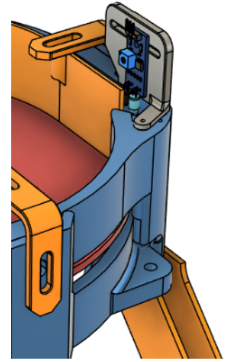
\includegraphics[width=5cm]{ch5/IR_Sensor_Placement.png}
    \caption{IR Sensor Placement}
    \label{fig:ir_sensor_placement}
\end{figure}
Another point of improvement was the placement of the IR sensor, which was redesigned to be adjustable. This adjustability allowed faster calibration and ensured accurate detection of beans at the table’s edge, further enhancing the system’s reliability and consistency. Initially, the rotating conveyor table is set at a fixed and slow speed to ensure that coffee beans are dropped into the inspection tray one-by-one. However, at this rate, the time travel time of the first bean dropped from the center of the table is very long. Thus, the group decided to add an IR sensor at the edge of the rotating table as seen in Figure X. The sensor’s responsibility is to detect if there is a bean at the edge. If there is no bean detected, the rotating table is set to a higher speed to expedite the process. On the other hand, if a bean is detected by the sensor, the rotation of the table is adjusted in such a way that it is able to drop the beans one-by-one onto the inspection tray. With this sensor integrated into the system, a higher speed can be set for the rotating table, minimizing the time travel of the beans from the center to the inspection tray, resulting in a faster sorting time for the first stage.

\subsection{Stage 1: Defect Sorting (Machine Vision and Inspection Tray)}

\begin{figure}[H]
    \centering
    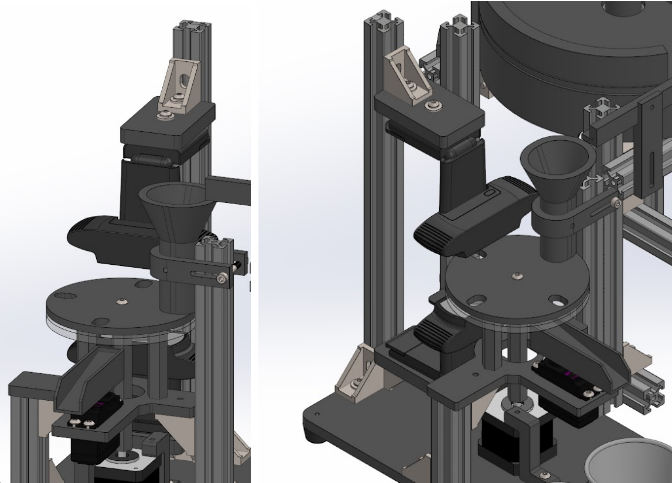
\includegraphics[width=12cm]{ch5/Inspection_Tray_Design.png}
    \caption{Inspection Tray 3D Design}
    \label{fig:inspection_tray_design}
\end{figure}

The inspection tray is the main component for the first-stage sorting mechanism. The inspection tray is used to support beans in a stable and constrained position for a short time, enabling the camera to take high-resolution images without motion blur. The NEMA 17 stepper motor drives the movement of the inspection tray, enabling accurate alignment with the vision system's image processing pipeline. The tray surface is created to reduce reflections and enhance contrast so that the camera can precisely detect defects like cracks, discoloration, or insect infestation. In addition, the surface is made of clear acrylic to allow a clear image for the camera positioned at the bottom of the tray. Lastly, a rotatable slider controlled by a 5V servo motor serves as the main segregator of the good beans from the defective beans. 

\subsection{Stage 2: Density Sorting (Precision Scale and Servo Mechanism)}
\label{sec:density_sorter}

% TODO: ADD FIGURE
\begin{figure}[H]
    \centering
    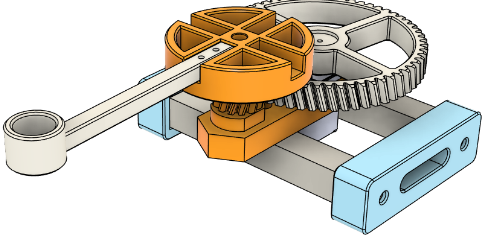
\includegraphics[width=12cm]{ch5/Density_Sorter_Mechanism_Design.png}
    \caption{Density Sorter Mechanism Design}
    \label{fig:density_sorter_design}
\end{figure}
The density sorter is the second-stage sorting system, tasked with sorting coffee beans according to their measured density. This is achieved by initially measuring each bean's mass using a precision weighing scale and volume using the computer vision. After calculating the density, the system triggers a sorting system powered by a geared 5V  servomotor, which sorts beans into various collection bins according to their classification. This sorting operation is such that high-density beans are kept separate from low-density beans. The density sorter's accuracy is verified by comparing the results of its classification to manual weighing measurements (ground truth data).

\begin{figure}[H]
    \centering
    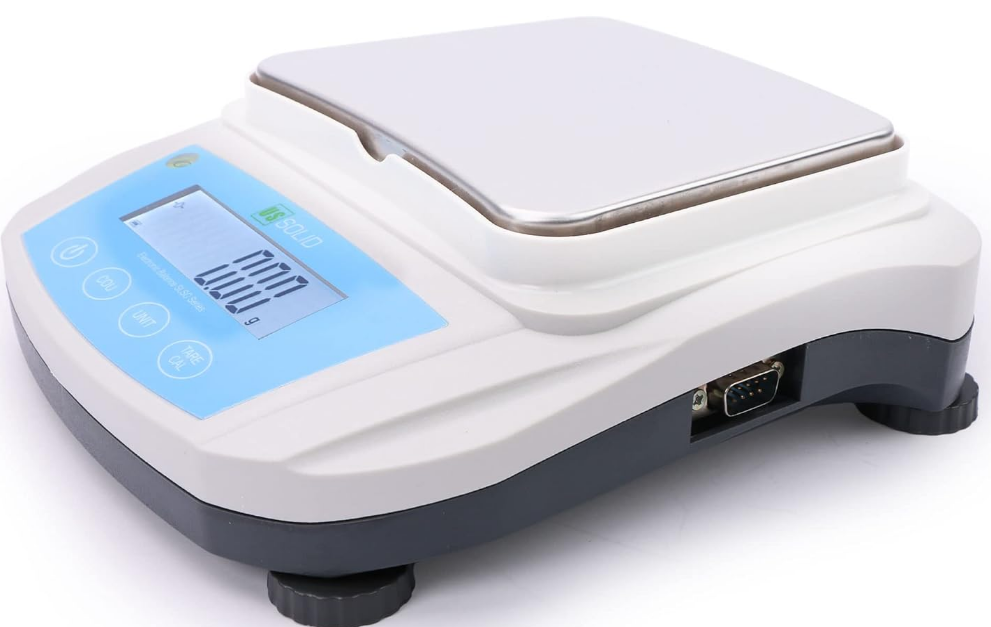
\includegraphics[width=9cm]{ch5/Precision_Scale.png}
    \caption{Precision Scale}
    \label{fig:precision_scale}
\end{figure}
The U.S. Solid Electronic Precision Balance (0.01g, 1200g capacity, RS232 port, AC/DC power) was selected for the density sorting mechanism because it is highly accurate, transmits data in real-time, and is well-calibrated. Its 0.01g precision guarantees accurate mass readings, which are critical to precise density calculations in sorting coffee beans. The RS232 port facilitates smooth integration with the microcontroller for automatic data processing and sorting decisions, minimizing manual errors. Its dual power source (AC and battery) also guarantees uninterrupted operation in different environments, making it a dependable and efficient part of the coffee bean sorting system.

\section{Hardware and Software Integration}

\subsection{Serial Communication}
\label{sec:serial_communication}
\begin{figure}[H]
    \centering
    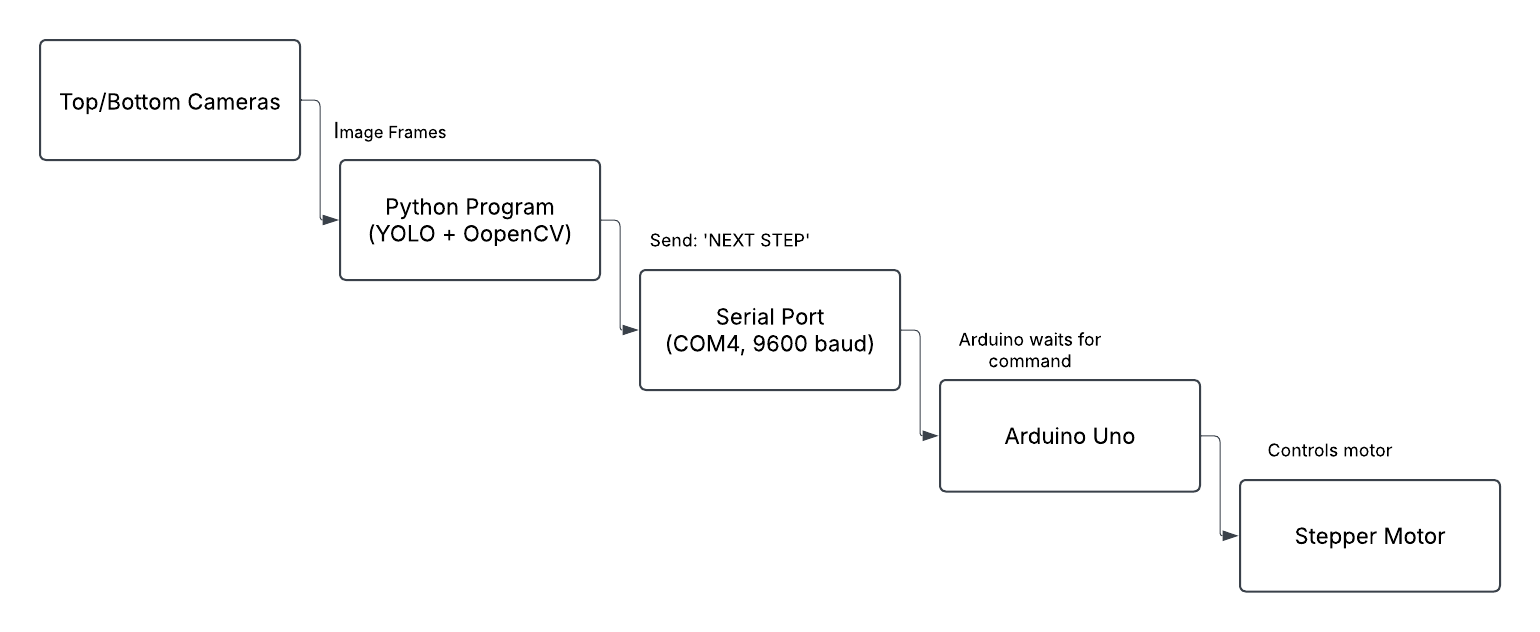
\includegraphics[width=12cm]{ch5/Serial_Communication_Flow_for_Stage_1_Classification.png}
    \caption{Serial Communication Flow for Stage 1 Classification}
    \label{fig:serial_comm_flow}
\end{figure}
The system is generally composed of hardware and software components. Hardware components are mainly responsible for collecting data from the coffee beans such as the camera and IR sensor, and the sorting mechanisms such as servo motors and stepper motors. On the other hand, the software components are the brain of the system which is mainly responsible for data processing such as image detection, defect classification of the beans, volume and density computation, and control of the mechanisms. Since the system has two major components, software and hardware, they should be integrated together for the system to be as effective. Thus, serial communication was utilized to integrate the hardware and software components of the system. Serial communication is a significant component in the system as it serves as the communication medium of the hardware and software. It enables real-time coordination between the software (YOLO-based image detection, classification, and density computation) and the hardware (running in Arduino microcontrollers). The said communication is established with the use of a USB serial interface using the pyserial library in Python. In addition, this is configured at a baud rate of 9600.

The system, specifically at the inspection tray mechanism where the YOLO detection and classification is implemented, has a function move\_stepper() responsible for sending the command from the Python code to the Arduino microcontroller. When the Arduino receive this command, it executes motor movement that allows the stepper motor to move at a certain angle that allows the camera to capture the bean. This function is crucial for the system as this is how each bean in the inspection tray is fed to the image processing side of the system. This movement rotates the mechanism holding the coffee beans, positioning the next bean beneath the top and bottom cameras for inspection. After the motor completes the movement, the Arduino will send back a message to the program running Python, signalling that the bean is ready for image capture and further processing. In addition, the Python script is continuously or constantly waiting for the Arduino’s message through the arduino.readline() function, ensuring seamless communication and faster processing. 


\subsection{Recommended Standard 232 (RS-232)}
\begin{figure}[H]
    \centering
    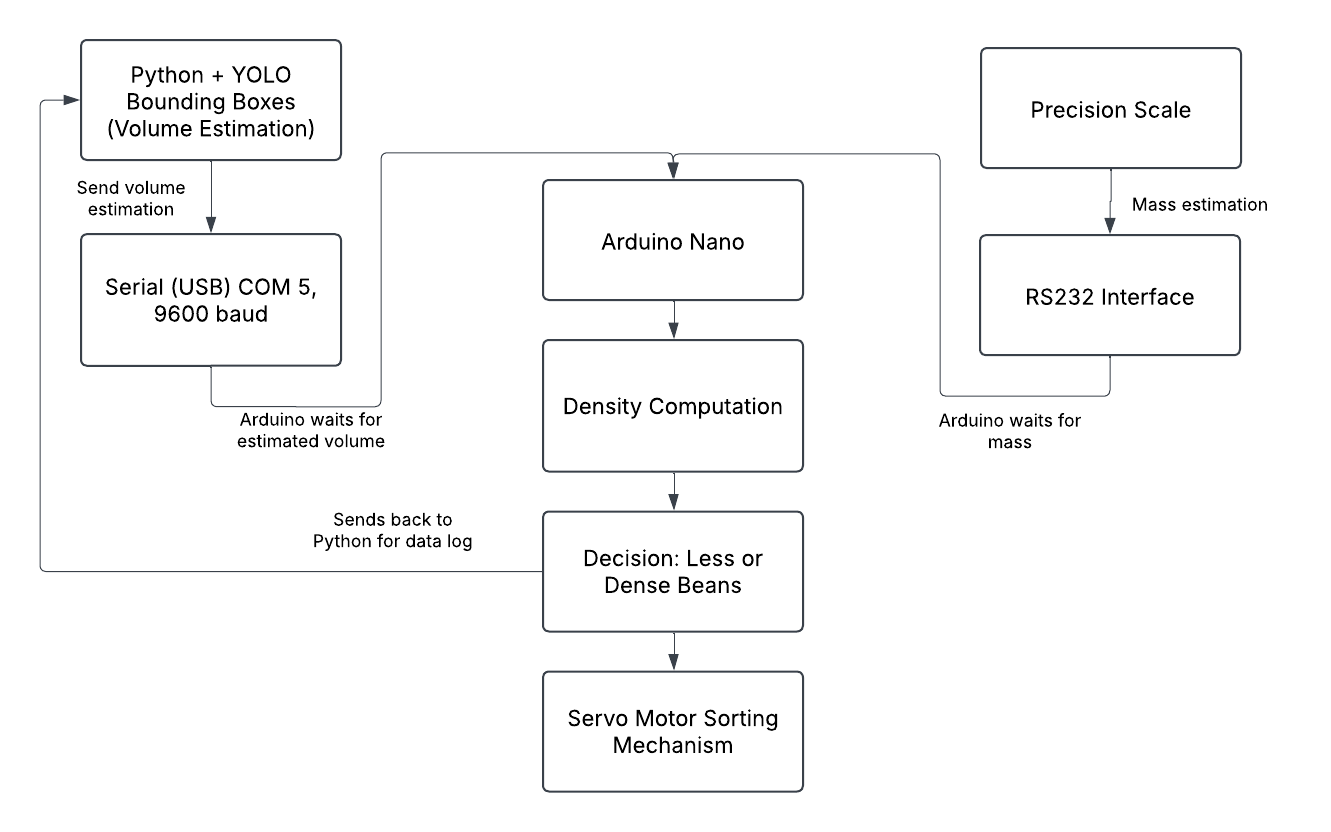
\includegraphics[width=12cm]{ch5/Precision_Scale_Integration_with_RS232.png}
    \caption{Precision Scale Integration with RS232 for Stage 2 Classification}
    \label{fig:rs232}
\end{figure}

The stage 2 classification is mainly composed of the sorting mechanism itself, and the precision scale to measure the mass of each bean. The bounding boxes from the stage 1 classification are used to estimate each bean’s volume. Additionally, the beans depth is also estimated through the IR sensor placed in the rotating conveyor table. With these measurements, the volume of each bean, the volume can be calculated using the Tri-axial Ellipsoid’s volume formula. 

The stage 2 classification, density-based sorting, is implemented using a combination of RS232 and USB serial communication. In this stage, each bean that has been classified as ‘Good’ from stage 1 is again sorted based on the density. The RS232’s main responsibility is to simultaneously record and pass the values to the Arduino Nano to compute the density. Subsequently, the data from the computations are the deciding factor whether to sort out the bean or not, depending on the predefined threshold for the system. 

\section{Prototype Setup}
\subsection{Actual Setup}

\begin{figure}[H]
    \centering
    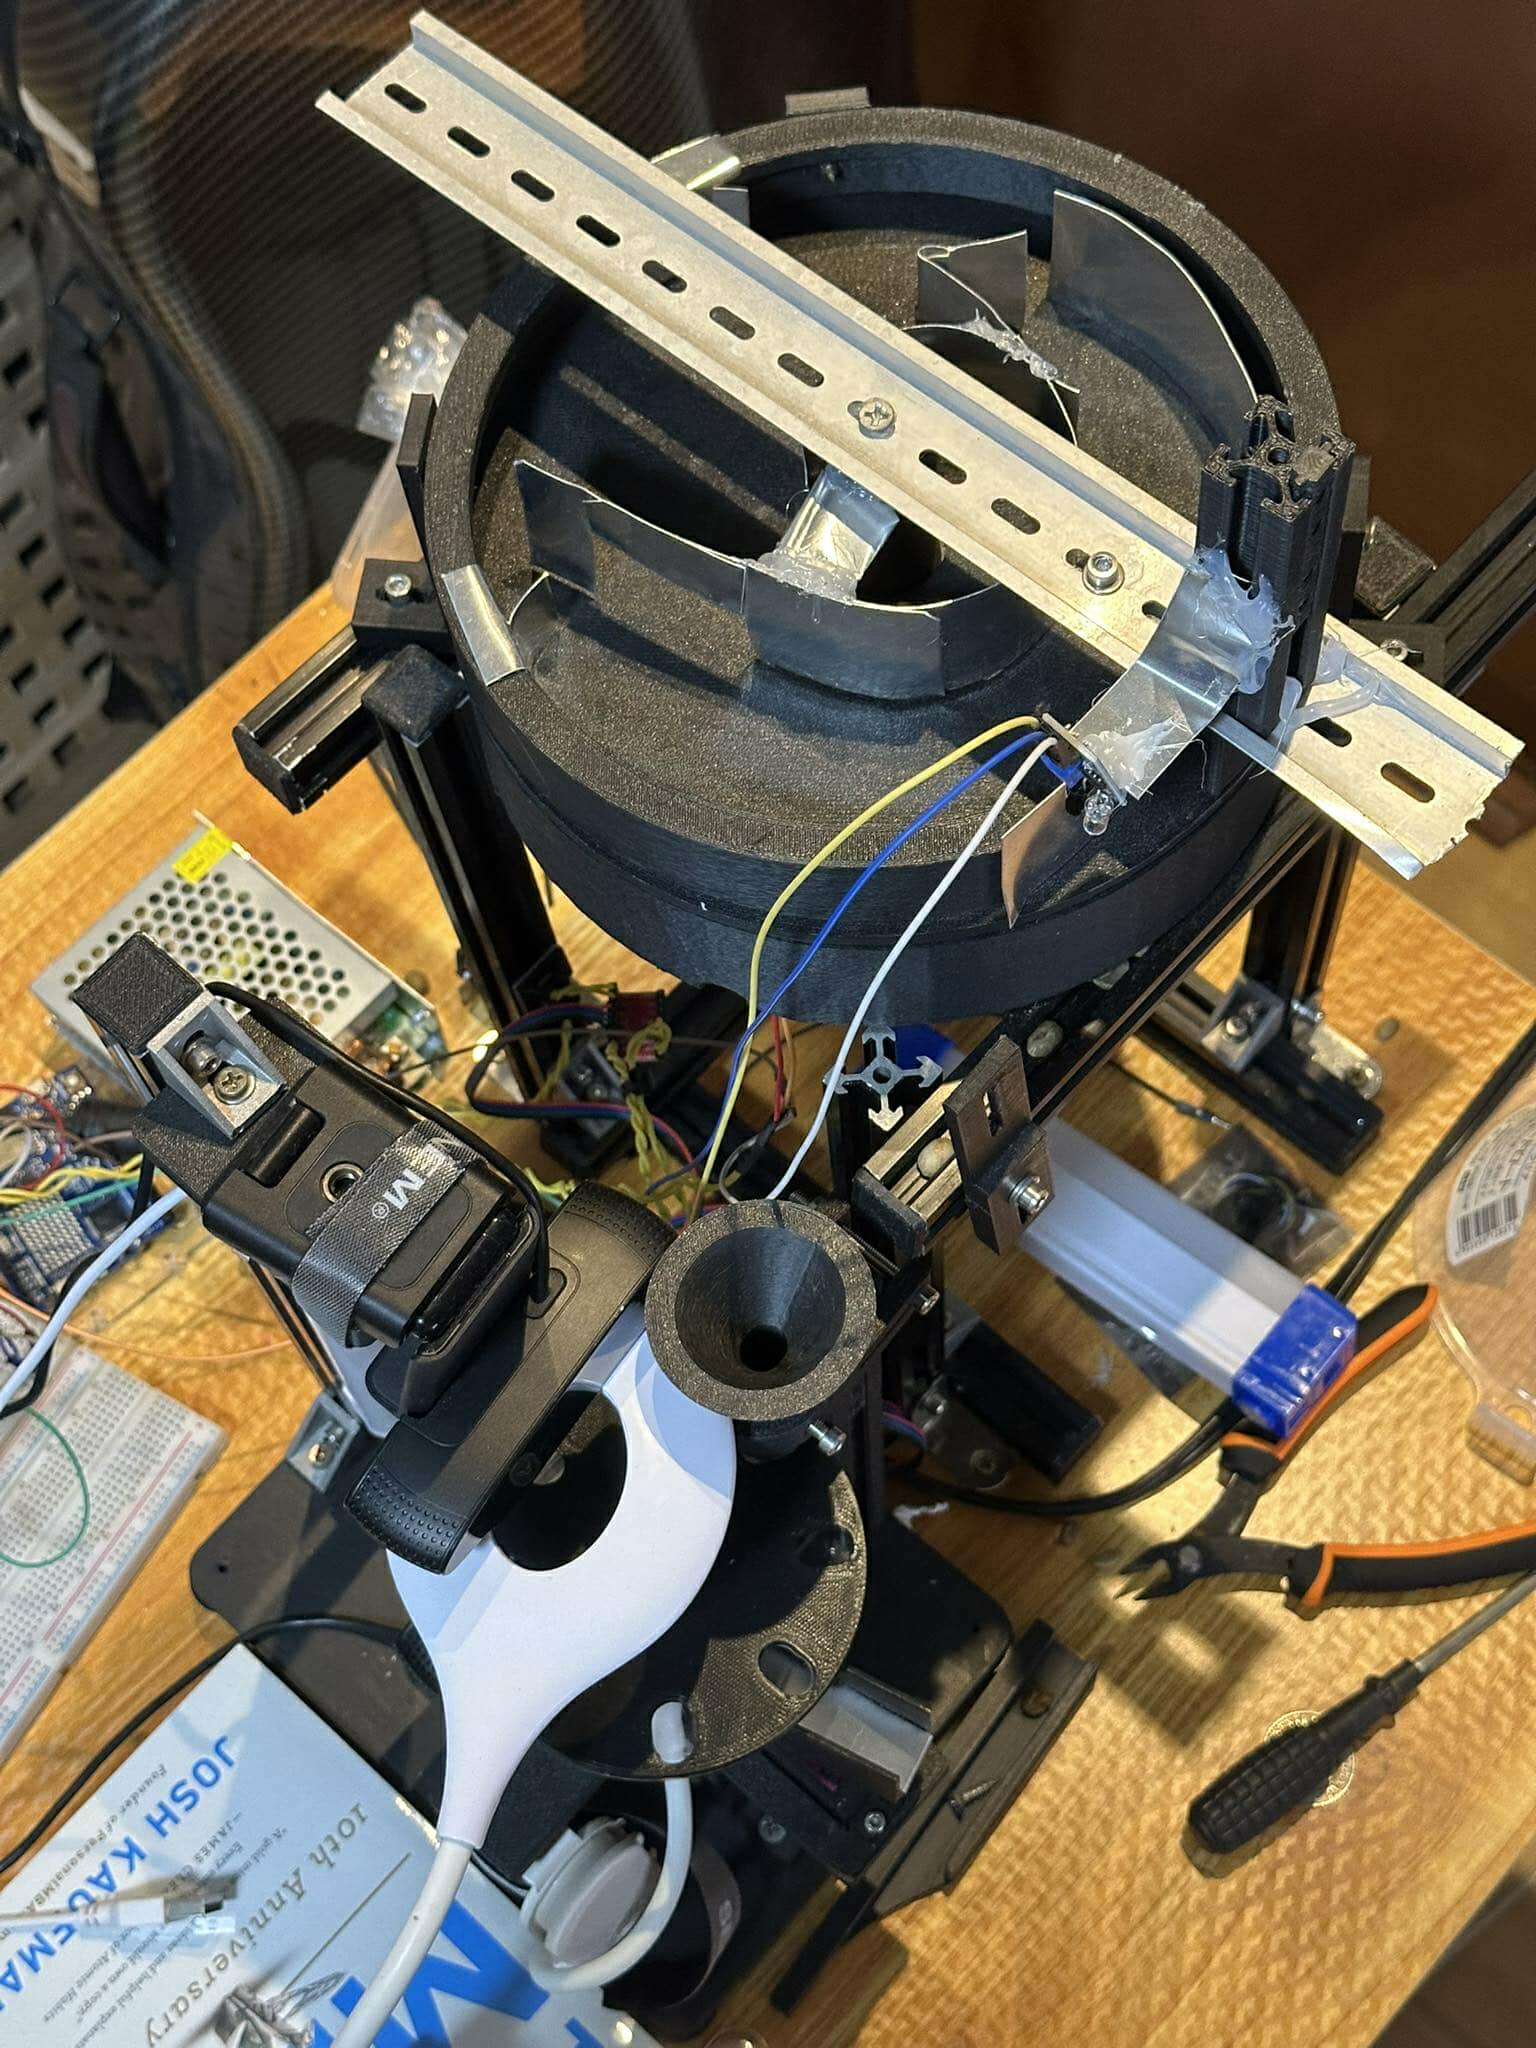
\includegraphics[width=9cm]{ch5/Actual_Setup_of_the_System.jpg}
    \caption{Actual System Setup (1st Iteration)}
    \label{fig:actual_setup_v1}
\end{figure}

\begin{figure}[H]
    \centering
    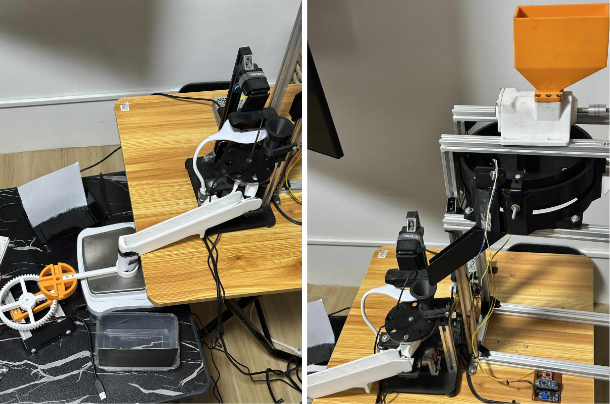
\includegraphics[width=9cm]{ch5/Actual_Setup_of_the_System_2.png}
    \caption{Actual System Setup (2nd Iteration)}
    \label{fig:actual_setup_v2}
\end{figure}

Physical integration of the automatic coffee bean sorter system comprises various integrated parts with the purpose of enabling effective, accurate, and methodical sorting in terms of visual defects as well as density categorization. The system involves integration of mechanical, electronic, and computer vision technologies for optimizing sorting. To begin the process, coffee beans are added to a revolving conveyor table, which is the main mechanism of transport used for feeding the beans into the inspection system. The conveyor features aluminum guides positioned strategically along it to ensure linear alignment of the beans as they travel. Linear alignment is required to avoid overlap and misclassification, since individual processing by the machine vision system is necessary for each bean.Once the beans travel further along the conveyor, they are conveyed onto the inspection tray. There, they are viewed in multiple perspectives by two high-definition cameras. A two-camera imaging process ensures improved defect detection by providing a full, thorough evaluation of the surface, shape, and texture of the bean. The images are then processed with a deep learning-based classification algorithm that classifies each bean as either defective or good according to predefined defect types like black beans, dried cherries, fungus damage, insect damage, sour beans, floaters, and broken beans. After classification, the system triggers the defect sorting mechanism, which physically takes out defective beans from the processing line. The mechanism includes a servo motor-powered sorting slide, which diverts defective beans into a distinct collection bin. Good beans that are classified are taken to the second level of sorting, which is density-based classification. At the density-based sorting level, good beans are weighed individually with a high-precision electronic balance. The U.S. Solid Electronic Precision Balance (0.01g, RS232) is embedded within the system to accurately weigh the mass of each bean. According to the calculation of density, beans are automatically sorted into corresponding collection bins using a second sorting mechanism regulated by a NEMA 17 stepper motor.

\subsection{Lighting Setup for Inspection Tray}

Lighting has a key importance in the image-based detection and classification system, specifically for the inspection tray. For the model to be more accurate and precise in classifying good and defective beans, correct lighting is important such that details like surface texture, color difference, and defects are properly rendered by the imaging system. Asymmetrical, unsteady, or low-quality lighting can create shadows, reflections, or overexposure, all of which lower the quality of input images and thus decrease the accuracy of object detection and classification models like YOLO. To improve the consistency and definition of images taken during inspection, the lighting arrangement above the inspection tray was refined incrementally throughout development. The refinements were intended to maximize the illumination conditions for both the top and bottom camera modules.


\begin{figure}[H]
    \centering
    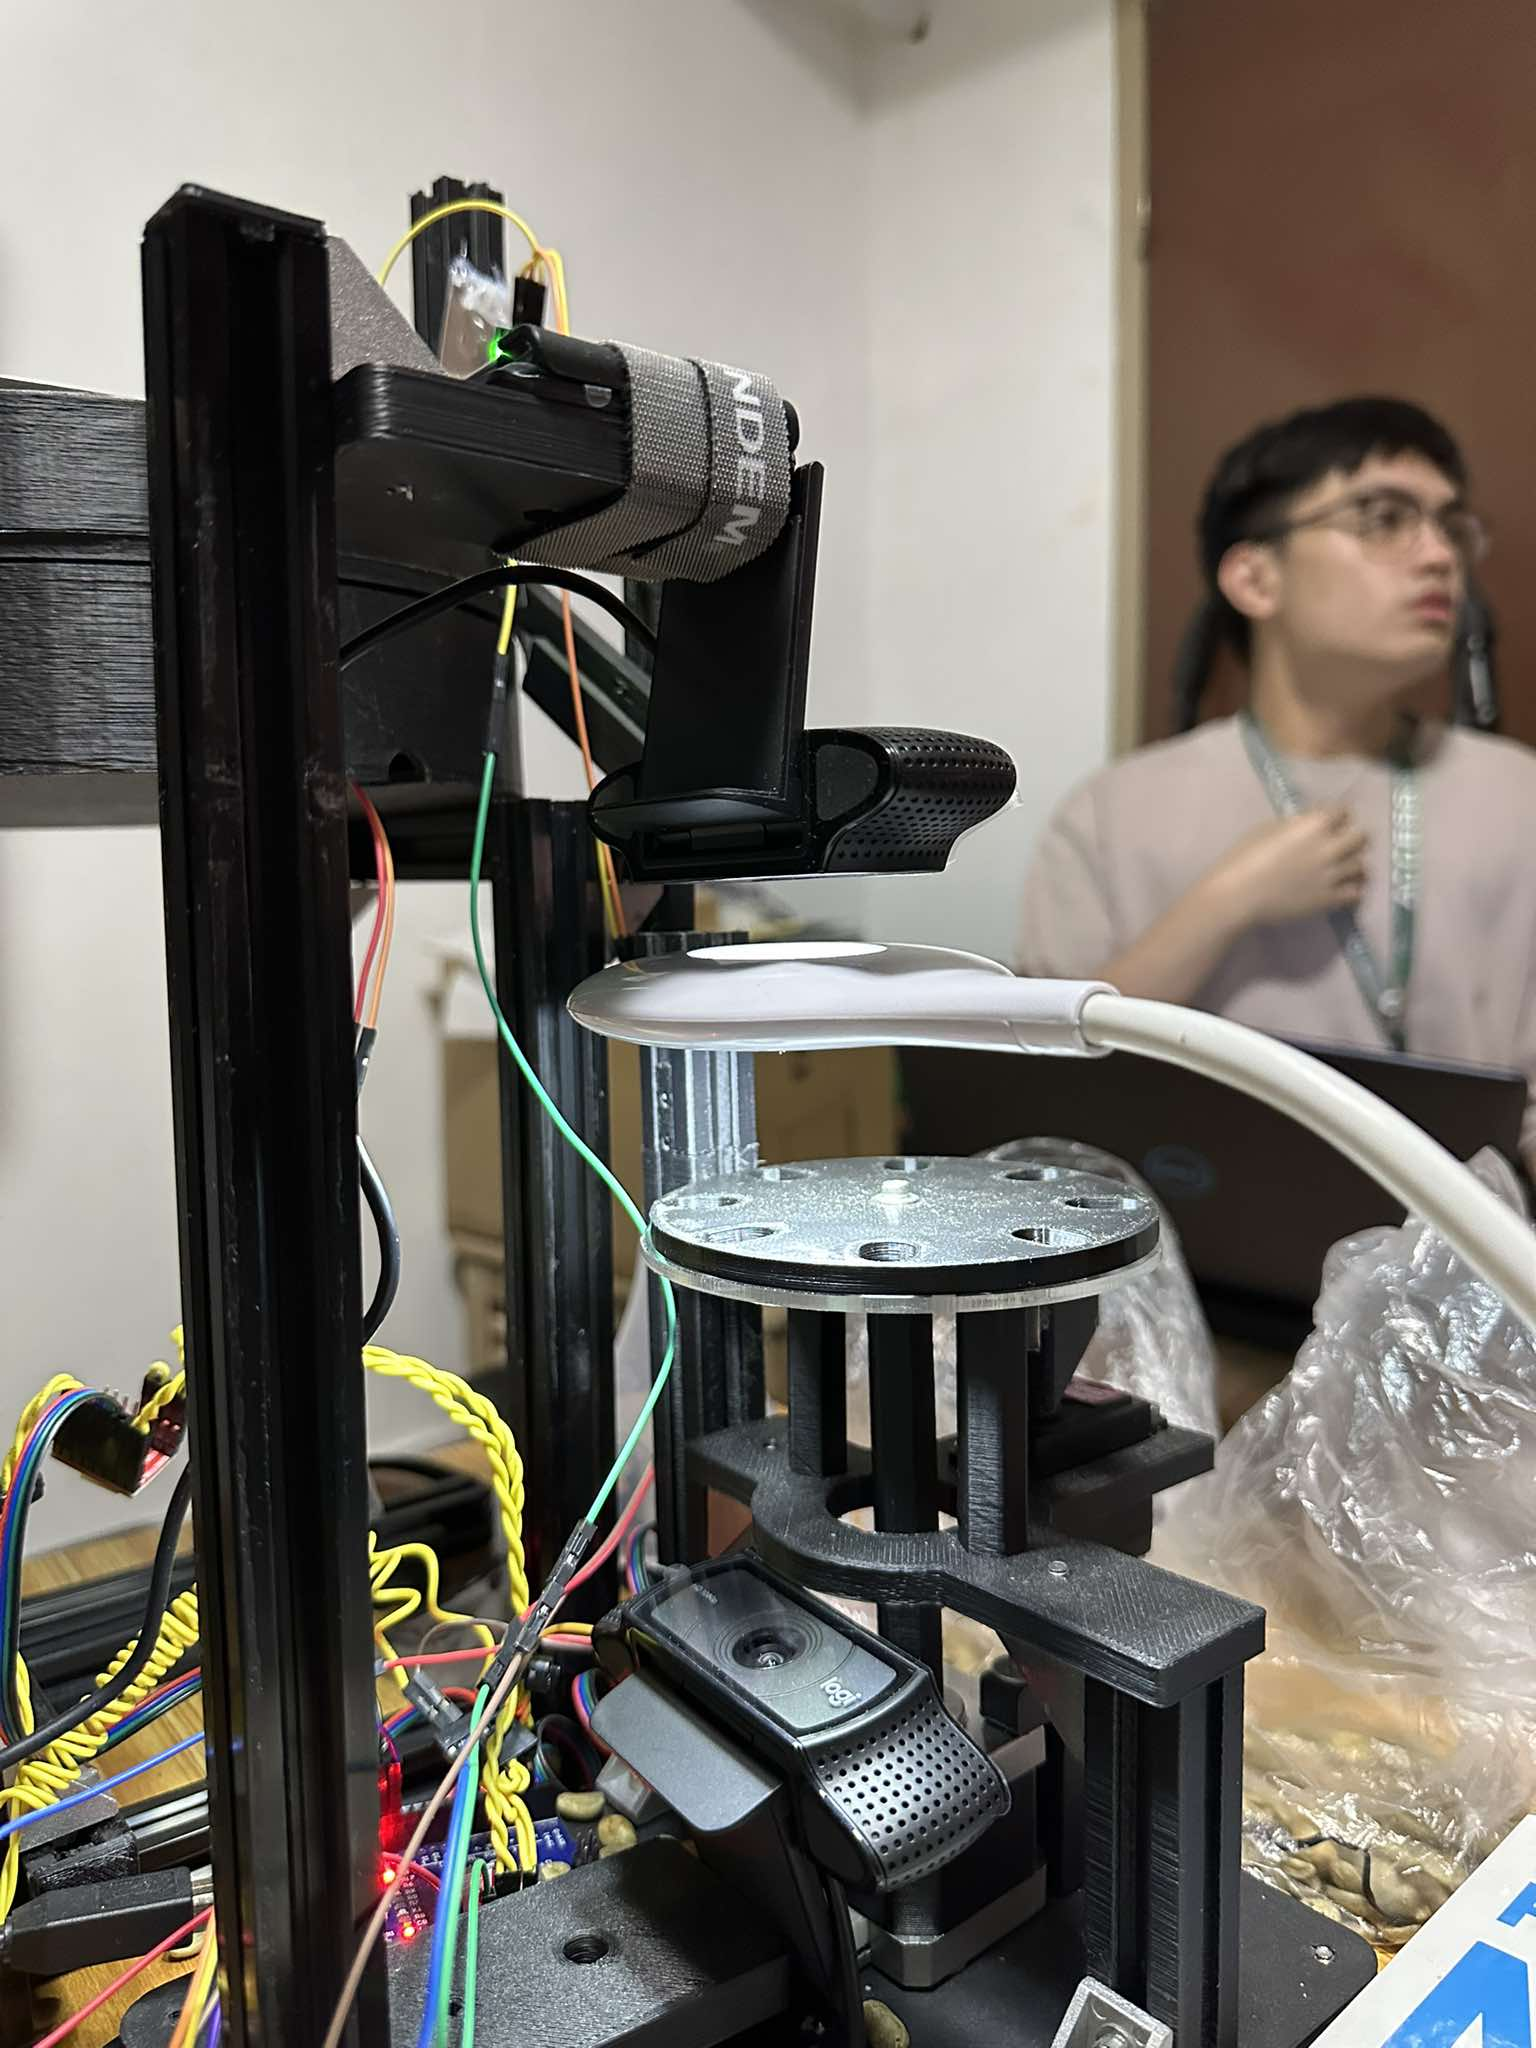
\includegraphics[width=9cm]{ch5/Initial_Lighting_Setup.jpg}
    \caption{First Iteration of Lighting Setup}
    \label{fig:first_lighting}
\end{figure}

Figure \ref{fig:first_lighting} shows the initial lighting setup that the researchers implemented on the system. The initial lighting arrangement was based on a single top-mounted LED lighting. Although the arrangement was more than bright enough for the top camera, it introduced random shadows and highlights onto the bottom camera. As a result, only one side of the bean is accurately inspected. These random elements impacted the model's performance in detecting bean contours and separating surface flaws, particularly for dark beans or reflective-surface beans.


\begin{figure}[H]
    \centering
    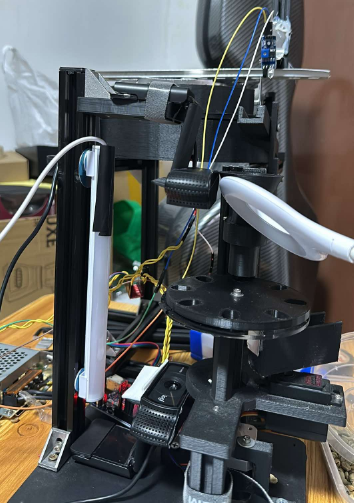
\includegraphics[width=9cm]{ch5/Modified_Lighting_Setup.png}
    \caption{Second Iteration of Lighting Setup}
    \label{fig:second_lighting}
\end{figure}

For the second iteration of the lighting setup, the researchers decided to add another LED strip lighting at the side of the inspection tray, while keeping the LED lighting mounted at the top. This provided good lighting for both top and bottom cameras. However, the view of the bottom camera is still a bit dark.


\begin{figure}[H]
    \centering
    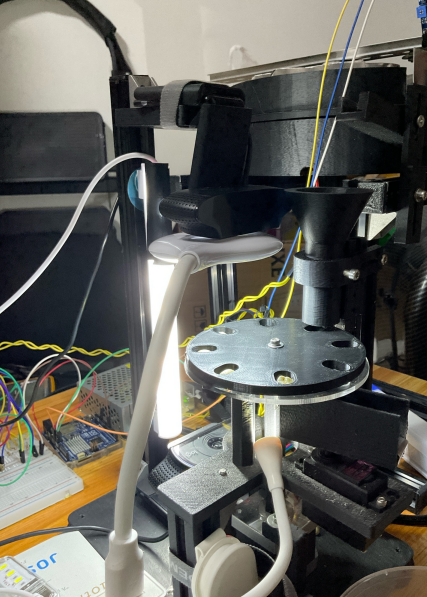
\includegraphics[width=9cm]{ch5/Final_Lighting_Setup.png}
    \caption{Final Iteration of Lighting Setup}
    \label{fig:final_lighting}
\end{figure}

To ensure that both camera views have sufficient lighting and avoid shadows, the researchers decided to use a total of three LED lights. One is a small ring light placed exactly above the inspection tray. Another LED light is a strip light placed at the side of the inspection tray to improve lighting at the side of each bean. Another small LED light is placed under the inspection tray to ensure that the bottom camera has enough lighting. Electrical tape was applied to the side of the acrylic plate to block excess lighting, thereby optimizing the lighting setup of the system.

\begin{figure}[H]
    \centering
    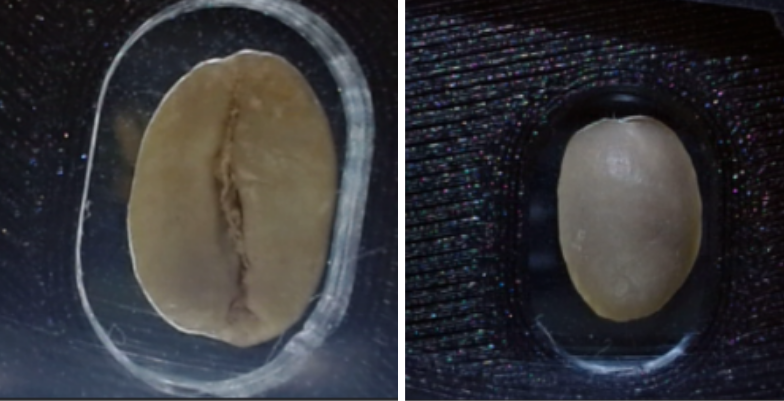
\includegraphics[width=9cm]{ch5/Top_and_Bottom_View_of_the_Cameras.png}
    \caption{Top and Bottom View of the Cameras}
    \label{fig:top_and_bottom}
\end{figure}

\subsection{System Operation}

The system operation follows a sequential process to ensure the effective sorting of green coffee beans (GCBs) based on its classification and density. The automated system consists of two primary stages: 1st Stage which is the machine vision-based classification and 2nd stage which is the density-based sorting.

The process beings in the inputting of unsorted GCBs (Contains good and defective beans) into the screw feeder, which regulates the controlled and consistent delivery of the beans into the rotary conveyor table. The conveyor table is designed with aluminum guides to ensure a linearized formation of the beans to mitigate jamming. This also ensures a controlled movement of beans, ensuring that they drop onto the inspection tray one at a time. As the bean goes towards the edge of the conveyor table, the IR sensors detects the beans and stops the rotation to ensure the one-by-one inspection of the beans, this also prevents clogging, and jamming once the beans are dropped into the inspection tray. 

The first phase involves machine-vision classification. Once the GCBs reach the inspection tray, each bean is analyzed one-by-one using a machine vision system consisting of top and bottom cameras. The system captures high-resolution images of the bean and processes the data to determine which classification it belongs. If the bean is identified as defective, a signal is sent to the servo motor, which redirects the bean into the defective bin for disposal, if the bean is classified as good, it then proceeds to the second phase of the system

The second stage involves density-based sorting, where each GCB's weight is measured using a precision scale, while its volume is determined by the bounding boxes from the first stage. These bounding boxes were used to estimate the dimensions of the beans and used the Ellipsoid volume formula for volume estimation.  

The sorting mechanism activates, directing beans into designated collection bins based on their density. High-density beans, often associated with specialty-grade quality, are separated from low-density, commercial-grade, or defective beans. 

\section{Prototype Testing}

\subsection{Sorting Speed}

\begin{figure}[H]
	\centering
	\begin{tabularx}{\textwidth}{p{0.3\textwidth}|p{0.2\textwidth}|p{0.2\textwidth}|p{0.2\textwidth}}
		\caption{Sorting Speed Testing Table} \label{tab:sorting_speed} \\
		\hline \hline
		\textbf{Test Condition} & \textbf{Conveyor Table Speed (RPM)} & \textbf{Inspection Tray Speed (RPM)} & \textbf{Sorting Speed (Beans per Minute)} \\
		\hline
		100\% Good Beans &  &  &  \\
		\hline
		75\% Good, 25\% Defective Beans &  &  &  \\
		\hline
		50\% Good, 50\% Defective Beans &  &  &  \\
		\hline
		25\% Good, 75\% Defective Beans &  &  &  \\
		\hline
		100\% Defective Beans &  &  &  \\
		\hline
	\end{tabularx}
\end{figure}

The sorting speed of the system will be determined by conducting at least five trials. Each trial will be exactly conducted for one minute. The number of beans sorted out within the time frame are considered as the sorting speed in beans per minute. Then, the average sorting speed from the five trials is computed. In each trial session, controlled variables such as motor speed of the inspection tray and rotating conveyor table are varied to observe the optimal setting for the system, ensuring that there are no beans jamming in the tray and fast enough to meet the minimum sorting speed. Table \ref{tab:sorting_speed} shows the different conditions for each trial to ensure that the sorting speed across different type of beans are considered. 

\subsection{Defect Sorting Accuracy}

To measure the system’s performance on defect sorting, two separate tests were performed. The first test was performed to measure the system’s accuracy on classifying the seven defect types including good beans. On the other hand, a second test was conducted to measure the system’s reliability on sorting out defective beans from good beans. In this test, there are only two classifications – defective beans and good beans. 

\begin{figure}[H]
	\centering
	\begin{tabular}{cc}
		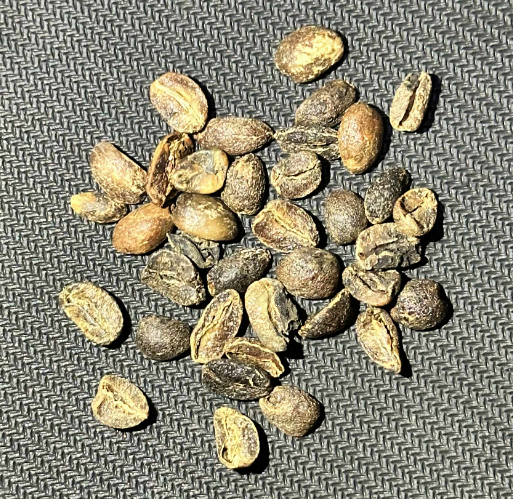
\includegraphics[height=0.2\textwidth]{ch5/Per-Classification Test Dataset/Black.png} &
		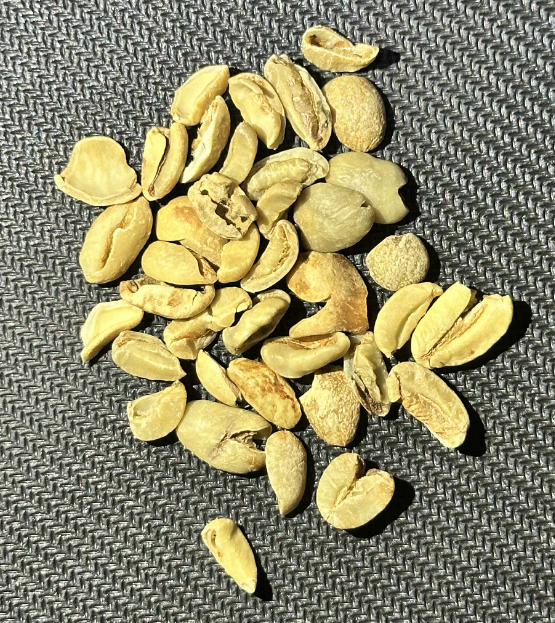
\includegraphics[height=0.2\textwidth]{ch5/Per-Classification Test Dataset/Broken.png} \\
		\textbf{Black - 30 Beans}  & \textbf{Broken - 30 Beans} \\[6pt]
	\end{tabular}
	\begin{tabular}{cc}
		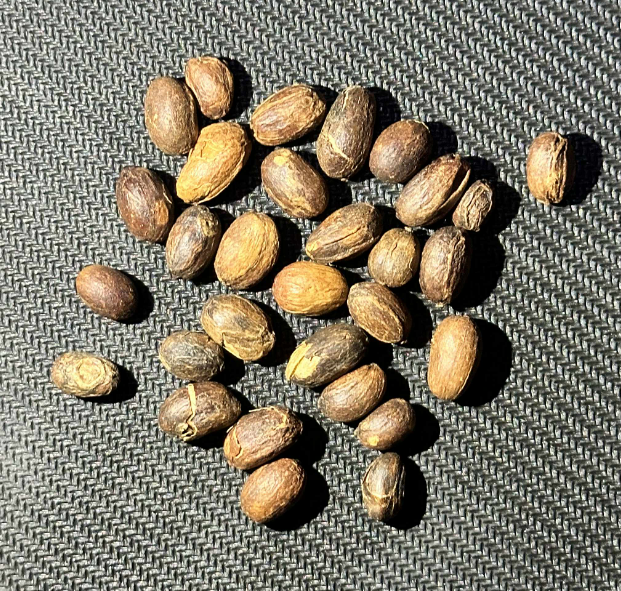
\includegraphics[height=0.2\textwidth]{ch5/Per-Classification Test Dataset/Dried Cherry.png} &
		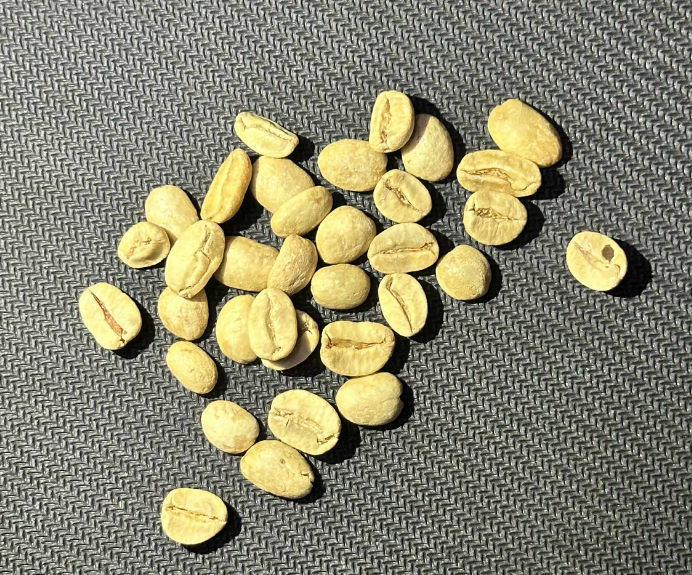
\includegraphics[height=0.2\textwidth]{ch5/Per-Classification Test Dataset/Floater.png} \\
		\textbf{Dried Cherry - 30 Beans}  & \textbf{Floater - 30 Beans} \\[6pt]
	\end{tabular}
	\begin{tabular}{cc}
		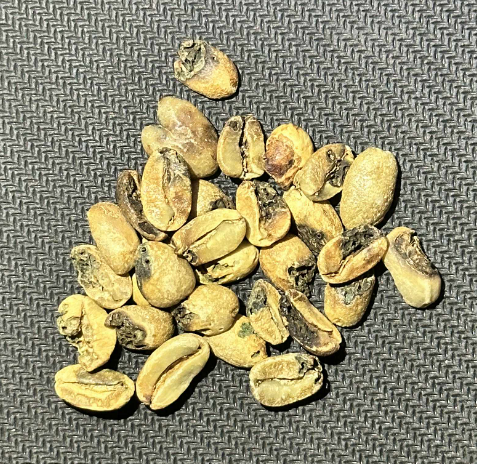
\includegraphics[height=0.2\textwidth]{ch5/Per-Classification Test Dataset/Fungus.png} &
		\includegraphics[height=0.2\textwidth]{ch5/Per-Classification Test Dataset/Good.png} \\
		\textbf{Fungus Damage - 30 Beans}  & \textbf{Good - 150 Beans} \\[6pt]
	\end{tabular}
	\begin{tabular}{cc}
		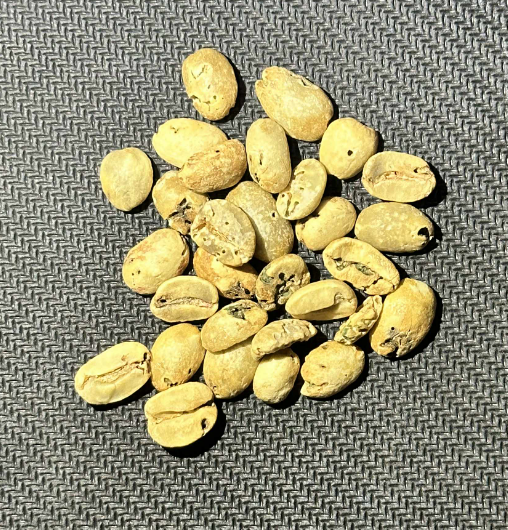
\includegraphics[height=0.2\textwidth]{ch5/Per-Classification Test Dataset/Insect.png} &
		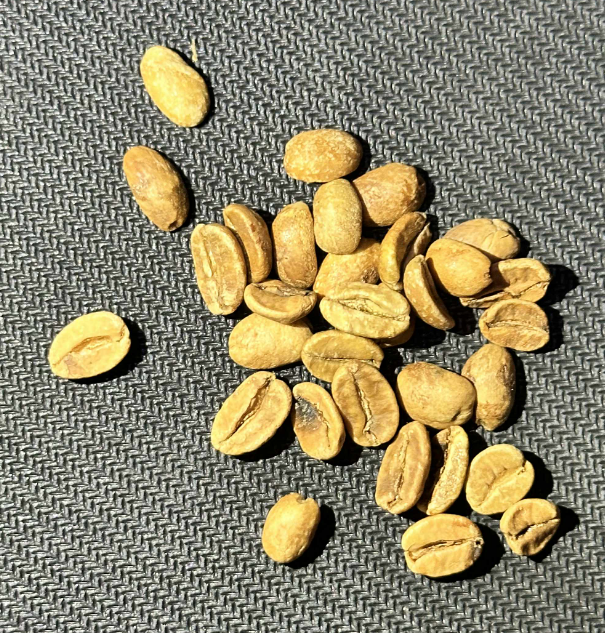
\includegraphics[height=0.2\textwidth]{ch5/Per-Classification Test Dataset/Sour.png} \\
		\textbf{Insect Damage - 30 Beans}  & \textbf{Sour - 30 Beans} \\[6pt]
	\end{tabular}
	\caption{Per-Classification	Test Dataset}
	\label{fig:per_classification_test_dataset}
\end{figure}

Table \ref{fig:per_classification_test_dataset} shows the actual test dataset used in the first test. This test was conducted using the top two performing models after training. Based on the 70-20-10 training, validation, test split, the researchers gathered 30 beans for each defect type, and 150 for good beans. The test consists of 5 trials with the same test set. Each trial was divided into 8 parts, corresponding to each classification. In this test, if one of the cameras detects the specific defect type being tested, it is considered as correctly classified. However, for good beans, both cameras should be able to classify it as good to be considered as a correct classification.

\begin{figure}[H]
	\centering
	\begin{tabular}{cc}
		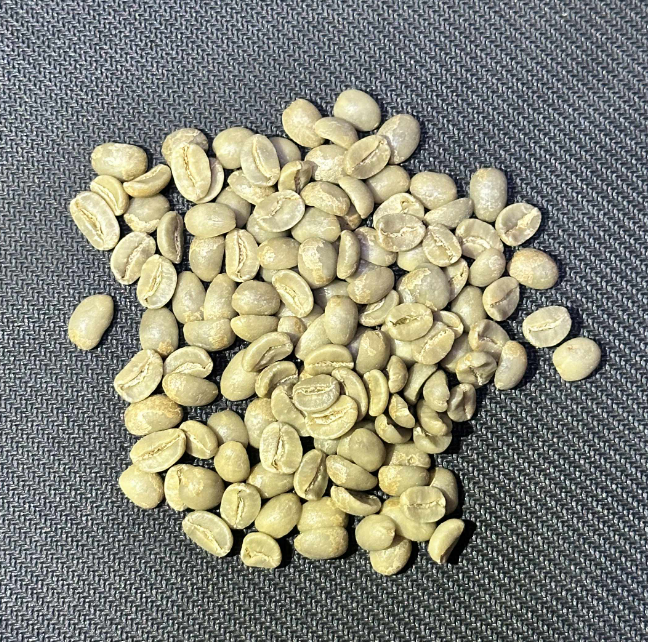
\includegraphics[height=0.2\textwidth]{ch5/Good vs. Defect Test Dataset/100-Good.png} &
		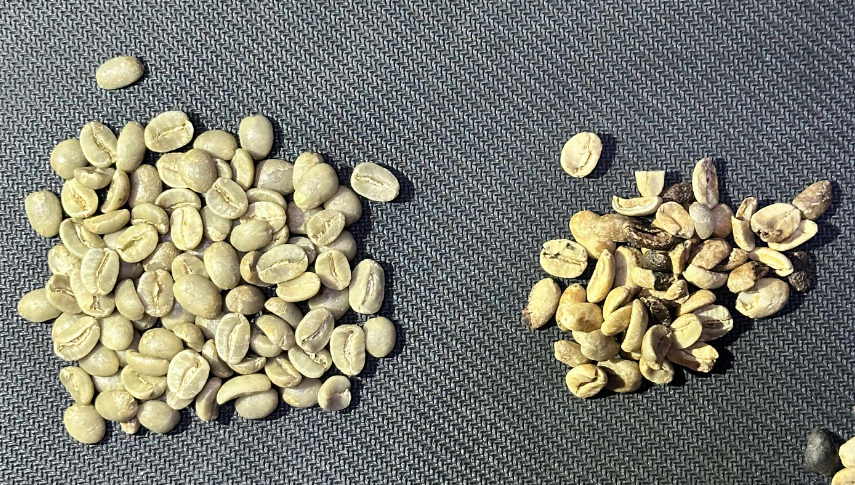
\includegraphics[height=0.2\textwidth]{ch5/Good vs. Defect Test Dataset/75Good-25Defect.png} \\
		\textbf{100\% Good}  & \textbf{75\% Good, 25\% Defects} \\[6pt]
	\end{tabular}
	\begin{tabular}{cc}
		\includegraphics[height=0.2\textwidth]{ch5/Good vs. Defect Test Dataset/50Goodt-50Defect.png} &
		\includegraphics[height=0.2\textwidth]{ch5/Good vs. Defect Test Dataset/25Good-75Defect.png} \\
		\textbf{50\% Good, 50\% Defects}  & \textbf{25\% Good, 75\% Defects} \\[6pt]
	\end{tabular}
	\begin{tabular}{cc}
		\includegraphics[height=0.2\textwidth]{ch5/Good vs. Defect Test Dataset/100-Defect.png} &
		\\
		\textbf{100\% Defects} & \\[6pt]
	\end{tabular}
	\caption{Good vs. Defective Test Dataset}
	\label{fig:good_vs_defective_test_dataset}
\end{figure}

The defect sorting accuracy by feeding 100 beans on each trial. For testing its accuracy for detecting good beans and defective beans, five trials are conducted containing 100 beans of good beans for the first trial, 75 good and 25 defects for the second trial, 50 good and 50 defects for the third trial, 25 good and 75 defects for the fourth trial, and 100 defects for the last trial. With these, the number of correctly classified and misclassified beans are logged into the system to compute for accuracy. 

\begin{figure}[H]
	\centering
	\begin{tabularx}{\textwidth}{p{0.3\textwidth}|p{0.2\textwidth}}
		\caption{Dataset Distribution for Overall Testing} \label{tab:dataset_distribution} \\
		\hline \hline
		\textbf{Bean Classification} & \textbf{Bean Count} \\
		\hline
		Good & 150 \\
		\hline
		Black &  30 \\
		\hline
		Broken & 30 \\
		\hline
		Dried Cherry & 30 \\
		\hline
		Floater & 30 \\
		\hline
		Fungus Damage & 30 \\
		\hline
		Insect Damage & 30 \\
		\hline
		Sour & 30 \\
		\hline
		\textbf{Total Beans} & \textbf{360} \\
		\hline
	\end{tabularx}
\end{figure}

Lastly, to assess the overall accuracy and reliability of the first stage, machine vision-based defect classification,  a trial consisting of a predefined dataset of 360 coffee beans was conducted. The good classification consists of 150 beans, while each defect, such as black, dried cherry, fungus, insect damage, sour, floater, and broken beans, consists of 30 beans as shown in Table \ref{tab:dataset_distribution}.

\subsection{Density Sorting Accuracy}

To assess the accuracy of the mechanism, it will rely on measuring the accuracy and the reliability of the density sorting mechanism in sorting out the dense beans to the less dense beans. To successfully determine the accuracy of the system, the basis will be the scale, where the system should be able to sort the dense beans to the less dense bean in relation to the detected weight in the scale. A successful system should be able to sort with an accuracy of 85\%.
